% =====================================================================
% JMLR submission source (single document; Appendix C is the supplement)
% Typeset with the OFFICIAL, UNMODIFIED jmlr2e.sty (JmlrOrg/jmlr-style-file).
% JMLR accepts ONLY a PDF at submission; compile this project in Overleaf
% (pdflatex + bibtex, default latexmk) and upload the resulting PDF.
%
% The `preprint' option only removes the volume/submitted/published header
% (supplied by the editors after acceptance); the layout is unchanged.
%
% The supplementary derivations are Appendix C, Sections S.2-S.8, placed
% after the conclusion and before the bibliography.
% The eight figures are 600 dpi JPEGs (3600 x 1920 px) with physical
% size 6.0 x 3.2 in, embedded 1:1 at width=\textwidth. Glyphs are
% rasterised: no nested PDF font subsets or transparency groups.
% JMLR-compliant type sizes (at least nine points) and horizontal legends
% placed below each subplot, outside the plotting area;
% bookmarks and lastpage are disabled so one free-tier Overleaf compile finishes.
% Display equations carry one \label each (eq:e01-eq:e50).
% rev25: figures rasterised to JPEG (nested PDF CID fonts / transparency
%        groups were dropped by some viewers of the compiled PDF).
% rev9: prose synchronized with the polished English Word manuscript;
%        equations, labels, citations and all mathematics unchanged.
% rev16: author-specified keywords; \acks{} states no funding; Theorem 7
%        statement moved after Theorem 6 (numbers and refs unchanged).
% rev17: redundant blank lines removed around equations / headings / floats;
%        rigid vertical glue in the preamble keeps all pages uniform.
% rev19: ~1.4k words of repeated prose removed.
% rev20: figures restored to [!t] (rev19 [p] deferred all 8 to the end of
%        the PDF); compact 6.0x3.20 in canvases.  Equations, numerical
%        results, theorems, figures, tables and references unchanged.
%
% BEFORE SUBMISSION (final-format checklist, jmlr.org/format/):
%   [x] \acks{} records no external funding and no competing interests
%   [ ] cover letter: disclose arXiv preprint and overlap with [1],
%       suggest 3-5 action editors and reviewers
%   [ ] fill \jmlrheading fields 4-6 and \editor{} after the AE is assigned
%   [ ] verify all 34 refs.bib entries against the original sources
%   [ ] check table IV (7 columns) does not overfill the text width
%   [ ] keep total pages < 35 (or justify in the cover letter if > 50)
%   [x] no placeholder text remains in \acks{} or \addr{}
%   [ ] proofread by a non-author (required by JMLR)
% =====================================================================
% Fast-compile build: suppress PDF bookmarks / index destinations.
% Removes the hyperref "Token not allowed in a PDF string" warnings and
% avoids writing a bookmark tree for 100+ labels. Internal links stay.
\PassOptionsToPackage{bookmarks=false,hyperindex=false}{hyperref}
\documentclass[twoside,11pt]{article}

% Official JMLR style file. DO NOT MODIFY jmlr2e.sty.
\usepackage[preprint]{jmlr2e}

% Additional packages must come AFTER jmlr2e (see the official sample.tex).
% jmlr2e already loads epsfig, amssymb, natbib, graphicx and hyperref.
\usepackage[utf8]{inputenc}
\usepackage[T1]{fontenc}
\usepackage{amsmath,amssymb,amsfonts}
\usepackage{booktabs}
\usepackage{longtable}   % S.8 symbol table may break across pages
\usepackage{url}
\urlstyle{same}
\graphicspath{{figs/}{../figs/}}
% A2: versioned archive URL (Zenodo version DOI or a GitHub release tag).
% This is the only place to edit the URL; Section 1 adds the commit hash.
\newcommand{\repourl}{\url{https://github.com/ShishuYin/minsep-participation/releases/tag/V1.0.1}}

\hypersetup{hidelinks}

% Uniform vertical spacing (rev17).  The article defaults carry stretchable
% glue (\parskip, \textfloatsep, \abovedisplayskip, ...), which spreads
% figures, headings and equations on short pages.  Fix them to small rigid
% values and use \raggedbottom so no glue is stretched.  jmlr2e.sty and its
% 10 pt caption skip are left untouched.
\raggedbottom
\setlength{\parskip}{0pt}
\setlength{\textfloatsep}{6pt}
\setlength{\intextsep}{6pt}
\setlength{\abovedisplayskip}{5pt}
\setlength{\belowdisplayskip}{5pt}
\setlength{\abovedisplayshortskip}{2pt}
\setlength{\belowdisplayshortskip}{2pt}
% rev33: four pairs of figures share one float each (two images, two
% captions, one figure environment). A single float is indivisible, so
% each pair stays on one page. Each pair is placed immediately after the
% first \ref to its first figure, and "!" forces placement there instead of
% letting the tall floats accumulate until the document ends. No figure is
% resized (the 9.5 pt type stays 9.5 pt) and jmlr2e.sty is untouched.
\setcounter{topnumber}{2}
\setcounter{totalnumber}{4}
\renewcommand{\topfraction}{1.0}
\renewcommand{\textfraction}{0.01}
\setlength{\floatsep}{2pt}

% Fast-compile build: relax line breaking to remove Overfull \hbox
% warnings in long inline-math paragraphs. No content is changed.
\tolerance=3000
\setlength{\emergencystretch}{1.5em}

% Supplementary appendix (merged into this file as Appendix C).
\newtheorem{slemma}{Lemma}[subsection]
\newtheorem{sprop}[slemma]{Proposition}
\newtheorem{scor}[slemma]{Corollary}
\newtheorem{sconj}[slemma]{Conjecture}
\newtheorem{srem}[slemma]{Remark}

% Title-page header. Under the preprint option only the copyright year and
% authors are printed; the volume and paper id are supplied by the production
% editor after acceptance, so fields 1 and 4-6 are left blank here.
\jmlrheading{}{2026}{}{}{}{}{Shishu Yin}
\ShortHeadings{Minimum-Separation Sampling Chains}{Yin}
\firstpageno{1}
\editor{}

\begin{document}
\title{On the Mixing Time and the Sampling Variance of Minimum-Separation Client Participation in Federated Learning}

\author{%
\name Shishu Yin \email ssyin@aufe.edu.cn \\
\addr School of Computer and Information Engineering,\\
Anhui University of Finance and Economics, Bengbu, China\\
ORCID: 0000-0002-4484-2379%
}
\maketitle
\begin{abstract}%
Minimum separation bars a selected client from the following $R$ rounds, inducing an $R$-th order Markov participation chain. We evaluate two time scales: the worst-case mixing time $\tau_{\mathrm{mix}}(R)$, governing burn-in, and the zero-frequency asymptotic variance $\sigma_i^2(R)$, governing estimation precision. For arbitrary positive conditional propensities and $2\leq R\leq N-2$, deterministic forgetting gives $\tau_{\mathrm{mix}}(R)\geq R$. Under uniform availability a companion-matrix reduction yields a degree-$R$ polynomial whose largest root modulus $\lambda_\star(R,N)$ governs both scales. A finite-dimensional lumping gives $\tau_{\mathrm{mix}}(R)\leq R+L(R,N)+\max\{0,\ln C(q)\}/|\ln\lambda_\star|$, with $C(q)$ independent of $|\mathcal{S}_R|$. This reduction also gives $\sigma_i^2(R)=(N-R)(N-R-1)/N^3$, decreasing in $R$ while $\tau_{\mathrm{mix}}$ increases. A covariance generating function gives the steady-state error of a constant-step-size linear estimator for $\eta\ll1-\lambda_\star$. For general non-uniform $p$ the stationary law follows from elementary symmetric polynomials, the boundary case $R=1$ has an explicit variance, and the aggregate variance splits into an explicit leading term and a Poisson-solve tail. Substituting $\tau_{\mathrm{mix}}$ into the finite-time bound of \citep{ref1} gives $\mathcal{O}([R+L]/t)$ on the main design regime.
\end{abstract}
% JMLR format: keywords follow the abstract, exactly as in published JMLR
% articles (e.g. Huang et al., JMLR 26 (2025) 1-61, p. 1). The official
% jmlr2e.sty keywords environment supplies the bold "Keywords:" label,
% 20 pt left/right inset and \small type; five comma-separated terms, no
% final period. Do not replace this with a hand-written macro.
\begin{keywords}
Markov chain mixing time, minimum-separation client sampling, federated learning, asymptotic sampling variance, non-reversible Markov chain spectra
\end{keywords}
\section{Introduction}
\textbf{Background and motivation.} In each round of federated learning the server selects one of $N$ clients; this sequence of selections is the client participation chain. Minimum separation excludes a client drawn at round $t$ from rounds $t+1,\dots,t+R$ \citep{ref1}. The rule fixes the admissible set at each round, so successive selections are dependent and a client's participation frequency differs from its availability probability. Differential-privacy accounting in deployed systems limits participation frequency \citep{ref2,ref3}, making the cooldown a scheduling constraint rather than a modelling choice. We study this participation chain under a fixed cooldown rule; the learning update it drives is not part of the analysis. The window state retains its initial configuration for $R$ rounds,
delaying forgetting, while forced non-repetition introduces negative
short-lag covariance with a positive tail beyond lag $R$. The quantity of interest is the time-averaged sampling frequency $\hat\nu_{T,i}=T^{-1}\sum_{s\le T}\mathbf{1}\{X_s=i\}$, the fraction of the first $T$ rounds in which client $i$ is selected. It estimates the stationary participation probability $\pi_{R,i}$, and its precision is the size of the fluctuation of $\hat\nu_{T,i}$ about $\pi_{R,i}$; for large $T$ this is governed by the zero-frequency asymptotic variance $\sigma_i^{2}(R)=\mathrm{Cov}_0+2\sum_{k\ge1}\mathrm{Cov}_k$ \citep{ref4}. The conditional propensities $p_i$ are fixed across rounds: the schedule removes the last $R$ selected clients from the admissible set and $p$ is renormalized over that set. Classical output analysis estimates $\sigma^{2}$ from a sample path
\citep{ref4,ref5}; deterministic cyclic and reshuffling schemes
\citep{ref6,ref7} and clustered sampling \citep{ref8} give closed-form
variance reductions, and importance-sampling policies are studied in
\citep{ref9}. Mixing-time analysis of MCMC detectors \citep{ref10,ref11} evaluates
the mixing time of a given transition rule. We evaluate the zero-frequency
variance of the $R$-th order chain generated by minimum separation over the
full intermediate range of $R$.

\textbf{Minimum separation as a Markov chain.} Minimum separation induces an $R$-th order Markov chain $P_R$ on the sliding window of the last $R$ sampled clients \citep{ref1}. We evaluate its mixing time and zero-frequency variance and derive the burn-in and step-size rules for the finite-time bound of that work.

\textbf{Main Contributions:} The main contributions of this paper are as follows.

\textbf{Terminology.} Throughout, \emph{uniform availability} means $p_i\equiv1/N$ for every client; the full model is defined in Section~3.1.
\begin{itemize}
\item For every conditional propensity vector with $p_i>0$ and $2\leq R\leq N-2$, the window retains its initial configuration for $R$ rounds, giving $\tau_{\mathrm{mix}}(R)\geq R$ (Theorem 1); the burn-in therefore grows at least linearly with $R$. The grouped extension is Corollary 1.
\item Under uniform availability, $\sigma_i^{2}(R)=(N-R)(N-R-1)/N^{3}$ and $2\sum_{k>R}\mathrm{Cov}_k=R(R+1)/N^{3}$ (Theorem 2, Corollary 2). The normalized integrated autocorrelation time $\tau_{\mathrm{int}}(R)=\sigma_i^{2}(R)/\mathrm{Cov}_0$ is then explicit and decreases with $R$ although $\tau_{\mathrm{mix}}$ increases.
\item For general non-uniform $p$ the $R=1$ stationary law and asymptotic variance are explicit (Theorem 3); a rational instance has $\sigma_i^{2}(1)/\sigma_i^{2}(0)\approx9.45$ (Proposition 1). The one-round marginal distance is bounded from below (Proposition 2).
\item Under uniform availability the window chain reduces on its centered
subspace to an $R\times R$ companion matrix whose degree-$R$ polynomial gives
$\lambda_\star(R,N)$ and
$\tau_{\mathrm{mix}}(R)\geq\max\{R,\lceil\ln2/|\ln\lambda_\star|\rceil\}$
(Theorem 4); the same reduction gives $\tau_{\mathrm{int}}(R)$. A resolvent
identity gives the steady-state mean-square error of a constant-step-size
linear estimator (Proposition 3, Remark 2), a covariance generating function
gives the error at any step size (Proposition 4), and a marginal recursion
covers $K>1$ clients per round (Corollary 3).
\item A finite-dimensional lumping gives a total-variation prefactor $C(q)$ independent of $|\mathcal{S}_R|=(N)_R$ and $\tau_{\mathrm{mix}}(R)\leq R+L(R,N)+\max\{0,\ln C(q)\}/|\ln\lambda_\star|$ (Theorem 5). Substituting into the finite-time bound \citep[Lemma~2]{ref1} gives $\mathcal{O}([R+L]/t)$ and a burn-in and step-size rule (Theorem 6). On $R\lesssim\sqrt{N/2}$ this sharpens to $\tau_{\mathrm{mix}}(R)=R+O(1)$ (Theorem~7); the idle-round variance is Corollary 4.
\item For general $p$ and every $R$, the stationary window distribution and client marginal have closed forms in elementary symmetric polynomials, and the aggregate asymptotic variance decomposes into an explicit leading term and a covariance tail \eqref{eq:e26} (Proposition 5).
\end{itemize}

\textbf{Organization.} Section~2 reviews related work, Section~3 defines the window chain and the three quantities, Section~4 states the main results and Section~5 proves them. Section~6 reports exact state-space iteration, simulation and labelled computational checks, and Section~7 states the scope and limitations. Appendices~A--B contain the Doeblin-type and tail-covariance bounds; Appendix~C contains the supplementary derivations and certificates.

\textbf{Code and reproducibility.} Scripts, fixed seeds and configuration files are pinned at \repourl{} (tag V1.0.1, commit 601a0c9).

\textbf{Notation.} $[N]=\{1,\dots,N\}$; $(N)_R=N!/(N-R)!$; $\|\cdot\|_{\mathrm{TV}}=\frac12\|\cdot\|_1$. We write $p=(p_1,\dots,p_N)$ with $p_i>0$ and $\sum_i p_i=1$, $p_{\min}=\min_i p_i$, and $\zeta_R$ for the stationary distribution of $P_R$; expectations are taken in stationarity. Here $\mathbf{1}\{\cdot\}$ is an indicator, $\mathbf{1}$ in matrix products the all-ones vector, and $\mathbf{I}$ the identity. The letter $l$ is a mixing lag, $t$ a round index, $\eta$ a step size, and $\eta_R(t)$ the one-round marginal; $\hat\nu_{t,i}$ is the $i$-th empirical frequency and $\tilde\nu_t$ the notation of \citep{ref1}. For $R=1$ we write $\pi_i$ for $\pi_{1,i}$; in stationarity $\nu_R(j)=\zeta_R(\{w:w_R=j\})$ coincides with $\pi_{R,j}$. We write $L(R,N)=\ln4/|\ln\lambda_\star(R,N)|$, $\alpha_{\mathrm{lr}}$ for the FedAvg learning rate, $\gamma$ for the idle-round probability, and $C(q)$ for the total-variation prefactor of Section~5.9.
Other symbols are defined where they first appear; Section~S.8 lists the
supplementary notation.

\section{Related Work}
Analyses of partial client participation differ in whether the chain-dependent constant is left unevaluated or computed for the specific participation rule. Three lines of work are relevant: deterministic cyclic and reshuffling schemes, which obtain acceleration from without-replacement sampling; Markov-sampling theory, which bounds complexity through a mixing or hitting time supplied as a primitive; and correlated-availability analyses, which characterize the bias induced by a non-uniform stationary distribution.

In \citep{ref6}, clients are partitioned into groups available in a fixed cyclic order, yielding $\widetilde{\mathcal{O}}(1/T^{2})$ rates for PL objectives when the group count is maximal. \citet{ref7} uses deterministic meta-epochs with client-level random reshuffling, bounding the statistical term by finite-population without-replacement sampling (Lemma B.1 of \citep{ref7}). In both works the variance reduction comes from using each component exactly once per epoch rather than from a stationary dependent process. Clustered sampling \citep{ref8} partitions clients into groups, and \citep{ref12} corrects for unknown participation probabilities.

Markov-sampling theory reduces dependence between samples to a scalar chain parameter. The oracle lower bound of \citep[Theorem~4.1]{ref13} is expressed through the hitting time $\tau_{\mathrm{hit}}$, which can be arbitrarily smaller than $|\mathcal{S}|\tau_{\mathrm{mix}}$; \citep{ref14} gives an algorithm-independent sample-complexity lower bound using a hitting-time bound $\tau$ as a primitive (Remark 3.2 of \citep{ref14} identifies $\tau=1$ with i.i.d. sampling). In \citep{ref15}, convergence bounds for stochastic gradient methods with arbitrary client participation contain a single term that depends on the participation rule and is retained in general form.

Client availability has also been modeled as correlated across rounds. In \citep{ref16}, availability follows an arbitrary finite-state Markov chain, the total error is split into an optimization error and a bias term $\chi^{2}_{\alpha\|p}\Gamma$ (Theorem 1 of \citep{ref16}), and Theorem 2 of \citep{ref16} shows that correlation slows convergence through the spectral quantity $\lambda(P)$; an aggregation rule with weights proportional to $\alpha_k/\pi_k$ removes the bias asymptotically (notation of \citep{ref16}). The quantity controlled there is the optimization error of the biased objective, $\lambda(P)$ is unspecified for a general availability chain. The objective-inconsistency analysis of \citep{ref17} and the biased-selection results of \citep{ref18} concern bias in the aggregated update rather than the time scales of the participation chain.

Minimum separation and the resulting $R$-th order window chain $P_R$ are studied in \citep{ref1}, where the analysis concerns the bias of a non-uniform stationary marginal and a debiasing rule, and the worst-case mixing time $\tau_{\mathrm{mix}}$ enters the finite-time bounds as a chain-level constant. Section~6 of \citep{ref1} conjectures that a larger $R$ yields a smaller $\tau_{\mathrm{mix}}$ \citep[App.~H]{ref1}. We evaluate $\tau_{\mathrm{mix}}$ and the zero-frequency variance of the empirical sampling frequency, the latter being the precision measure for a time-averaged frequency estimate.

Time-varying and unknown client-to-server connection availability, including Markovian and cyclic unreliable patterns, is treated in \citep{ref19}. That line studies convergence and bias of the learning update under arbitrary connection dynamics. \citet{ref27} cast client sampling as online learning with bandit feedback and minimize the \emph{sampling variance} by an online stochastic mirror-descent rule, with both simulated and real-data experiments.

The tools used below are developed elsewhere. They include mixing-time and
spectral-gap bounds \citep{ref29,ref30}, Hoeffding-type concentration with an
absolute-gap variance proxy \citep{ref28}, the Markov chain CLT
\citep{ref4,ref26,ref24}, MCMC output analysis and batch-means estimation
\citep{ref31,ref32}, and Markovian stochastic optimization
\citep{ref33,ref34}.

\section{The Participation Chain and Three Quantities}
\subsection{\texorpdfstring{The $R$-th order chain}{The R-th order chain}}
Consider $N$ clients and a baseline in which exactly one client is drawn in each round. A client drawn in round $t$ is excluded from rounds $t+1,\dots,t+R$, where $0\leq R\leq N-2$. Let $X_t$ denote the client sampled at round $t$ and define the window state $Y_t=(X_t,X_{t-1},\dots,X_{t-R+1})$. Its state space is $\mathcal{S}_R=\{(w_1,\dots,w_R): w_j\in[N]\ \text{distinct}\}$, of cardinality $|\mathcal{S}_R|=(N)_R$; the first component of a window is the most recent draw, and the one-step transition probabilities, collected in the transition matrix $P_R$, are
\begin{equation}\label{eq:e01}
P_R\big((I_1,\dots,I_R)\to(I_0,I_1,\dots,I_{R-1})\big) =\dfrac{p_{I_0}}{\sum_{j\notin\{I_1,\dots,I_R\}}p_j},\quad I_0\notin\{I_1,\dots,I_R\},
\end{equation}
and zero otherwise. For $R=0$ this reduces to i.i.d. sampling $X_t\sim p$. By \citep[Lemma~1]{ref1}, $P_R$ is irreducible and aperiodic for $R\leq N-2$ and has a unique strictly positive stationary distribution $\zeta_R$; for $R=N-1$ the chain is a deterministic $N$-cycle and is periodic. Unless stated otherwise we assume $2\leq R\leq N-2$, and we write $\pi_{R,i}=\mathbb{P}_{\zeta_R}(X_t=i)$ and $\nu_R(j)=\zeta_R(\{w:w_R=j\})$.

Given a window $w$, the next draw is $p$ renormalized over the admissible set, so $p_i$ is not the marginal selection probability and $\pi_{R,i}\neq p_i$ for $R>0$. Every admissible client is assumed available in every round; idle rounds are treated in Section~4.14, and real eligibility need not be independent of the cooldown schedule. \emph{Uniform availability} means $p_i\equiv1/N$ for every client, in which case the next draw is uniform on the admissible set and $\pi_{R,i}=1/N$ by permutation symmetry. All results below concern the chain $P_R$ of \eqref{eq:e01}.

\subsection{Mixing time, marginal distance, and asymptotic variance}
With the worst-case-initial-state convention of \citep[Def.~4]{ref1} and \citep[Def.~2.2]{ref13}, and at the conventional mixing-time accuracy $1/4$, define
\begin{equation}\label{eq:e02}
d_{\mathrm{TV}}(P_R^{l},\mathbf{1}\zeta_R^{\top}) =\max_{w\in\mathcal{S}_R}\|P_R^{l}(w,\cdot)-\zeta_R\|_{\mathrm{TV}},\quad t_{\mathrm{mix}}(\epsilon;R) =\inf\{l\geq1:\ d_{\mathrm{TV}}(P_R^{l},\mathbf{1}\zeta_R^{\top})\leq\epsilon\},
\end{equation}
and write $\tau_{\mathrm{mix}}(R):=t_{\mathrm{mix}}(1/4;R)$, omitting the argument $R$ when it is clear. Accuracy is denoted by $\epsilon$; the value $1/4$ is conventional and affects only constant factors, not the $R$-dependence. For $0\leq R\leq N-2$ the chain is finite, irreducible and aperiodic (or i.i.d.\ at $R=0$), and the Markov chain CLT gives
\begin{equation}\label{eq:e03}
\sqrt{T}\big(\hat\nu_{T,i}-\pi_{R,i}\big) \Rightarrow\mathcal{N}(0,\sigma_i^{2}(R)),\quad \sigma_i^{2}(R) =\mathrm{Cov}_0+2\sum_{k\geq1}\mathrm{Cov}_k,
\end{equation}
with $\mathrm{Cov}_0=\pi_{R,i}(1-\pi_{R,i})$ and $\mathrm{Cov}_k=\mathbb{E}_{\zeta_R}[\bar f_i(X_0)\bar f_i(X_k)]$ for $\bar f_i=\mathbf{1}\{\cdot=i\}-\pi_{R,i}$.

The mixing time $\tau_{\mathrm{mix}}(R)$ is the worst-case number of rounds
until the full window-state law is within total-variation distance $1/4$ of
stationarity, and sets the burn-in before a time average can be treated as
stationary. The one-round marginal distance
$\|\eta_R(t)-\pi_R\|_{\mathrm{TV}}$ is its projection onto the current draw. The third quantity is the precision of
$\hat\nu_{T,i}=T^{-1}\sum_{s\le T}\mathbf{1}\{X_s=i\}$ as an estimator of
$\pi_{R,i}$: $\sigma_i^{2}(R)$ is the zero-frequency ordinate $S_{f,f}(0)$
of the spectral density, and
$\tau_{\mathrm{int}}(R)=\sigma_i^{2}(R)/\mathrm{Cov}_0$.

\textbf{Remark 1.} Let $g$ map a window state to its first component. Let $\mu_0$ be the initial law on window states, which need not be stationary. Then $\eta_R(t)=\mu_0P_R^{t}g^{-1}$ and $\pi_R=\zeta_R g^{-1}$; since $\|\mu_0P_R^{t}-\zeta_R\|_{\mathrm{TV}}\leq d_{\mathrm{TV}}(P_R^{t},\mathbf{1}\zeta_R^{\top})$, contraction of total variation yields $\|\eta_R(t)-\pi_R\|_{\mathrm{TV}}\leq d_{\mathrm{TV}}(P_R^{t},\mathbf{1}\zeta_R^{\top})$. Starting from $\mu_0=\zeta_R$ the left-hand side vanishes identically, so the inequality gives no information under a stationary initialization. The inequality is one-directional: the marginal distance is at most the window-state distance, so fast mixing of the window state implies fast marginal convergence; the reverse implication does not hold.

\section{Main Results}
\subsection{\texorpdfstring{The mixing-time lower bound grows with $R$}{The mixing-time lower bound grows with R}}
\textbf{Theorem 1.} Let $p_i>0$ for all $i$, $N\geq4$ and $2\leq R\leq N-2$. Then
\begin{equation}\label{eq:e04}
\tau_{\mathrm{mix}}(R)\geq R,\qquad \tau_{\mathrm{mix}}(0)=1.
\end{equation}
Moreover, for every $p_i>0$ and every $1\leq t\leq R-1$, $\max_w\|P_R^{t}(w,\cdot)-\zeta_R\|_{\mathrm{TV}}\geq1-1/N$. The bound is independent of $p$; its only size condition is $N\geq R+2$, implied by $2\leq R\leq N-2$, so $N\geq4$ follows. The bound therefore applies to every positive conditional propensity vector. The grouped extension is Corollary 1. The proof, given in Section~5.1, uses only the fact that the window retains the initial configuration in its trailing positions through step $R-1$. At $R=N-1$ the chain is periodic and $\tau_{\mathrm{mix}}$ is not finite.

Under uniform availability ($p_i\equiv1/N$) $\tau_{\mathrm{mix}}(1)=1$ as well (see Section~5.1). Theorem~1 assumes $2\leq R\leq N-2$, so $R=1$ lies outside its scope for every $p$; for non-uniform $p$ the mixing time at $R=1$ can be arbitrarily large (Remark~4).

\textbf{Corollary 1.} Let $N=M_{\mathrm{grp}}S_{\mathrm{grp}}$ clients be arranged in $M_{\mathrm{grp}}$ disjoint groups of $S_{\mathrm{grp}}$ clients, let one group be sampled in each round with all its clients participating, and let the minimum separation act on groups. If $2\leq R\leq M_{\mathrm{grp}}-2$, then $\tau_{\mathrm{mix}}(R)\geq R$.

\subsection{\texorpdfstring{Sampling variance decreases with $R$ under uniform availability}{Sampling variance decreases with R under uniform availability}}
\textbf{Theorem 2.} Let $p_i\equiv1/N$ and $0\leq R\leq N-2$. Then for every client $i$,
\begin{equation}\label{eq:e05}
\sigma_i^{2}(R)=\dfrac{(N-R)(N-R-1)}{N^{3}},
\end{equation}
which is strictly decreasing in $R$, with $\sigma_i^{2}(0)=(N-1)/N^{2}$. The identity follows from the Markov chain central limit theorem (CLT) stated in \eqref{eq:e03}. At the periodic endpoint $R=N-1$ the chain is a deterministic $N$-cycle, the covariance series is not absolutely summable and the CLT does not apply; a direct counting argument instead gives $\lim_{T\to\infty}T\,\mathrm{Var}(\hat\nu_{T,i})=0$ (Section~5.2), which agrees with substituting $R=N-1$ into \eqref{eq:e05}. Theorem~2 is stated for the aperiodic range $0\leq R\leq N-2$, where the CLT holds.

\textbf{Corollary 2.} Under the assumptions of Theorem 2, the tail covariance and its decomposition are
\begin{equation}\label{eq:e06}
2\sum_{k>R}\mathrm{Cov}_k=\dfrac{R(R+1)}{N^{3}}>0,\quad \pi_{R,i}(1-\pi_{R,i})-2R\pi_{R,i}^{2}=\dfrac{N-1-2R}{N^{2}}.
\end{equation}
$\pi_{R,i}=1/N$ under Theorem 2. The second expression in \eqref{eq:e06}, $\pi_{R,i}(1-\pi_{R,i})-2R\pi_{R,i}^{2}=(N-1-2R)/N^{2}$, can be negative for $R>(N-1)/2$; the positive tail term in \eqref{eq:e06} compensates. Writing $\rho=R/N$, Theorem 2 gives $\sigma_i^{2}(R)/\sigma_i^{2}(0)=(1-\rho)(1-R/(N-1))\approx1-2\rho$ for small $\rho$. Under uniform availability $\mathrm{Cov}_0=\pi_{R,i}(1-\pi_{R,i})$ is independent of $R$, so this ratio is the normalized integrated autocorrelation time $\tau_{\mathrm{int}}(R)$ of Section~3.2: $\tau_{\mathrm{int}}(R)=1+2\sum_{k\geq1}\mathrm{Cov}_k/\mathrm{Cov}_0$, defined for $0\leq R\leq N-2$ and equal to $1$ at $R=0$. This convention, with $\tau_{\mathrm{int}}(0)=1$, differs by a factor of two from the Sokal normalization $\frac{1}{2}+\sum_{k\geq1}\mathrm{Cov}_k/\mathrm{Cov}_0$. It decreases with $R$ even though Theorem 1 gives $\tau_{\mathrm{mix}}(R)\geq R=\rho N$. The positive tail term arises at lag $R+1$: client $i$, released from the cooldown window, is admissible while the $R$ most recent draws remain forbidden, so its conditional selection probability exceeds stationarity.

\subsection{A complementary Doeblin-type bound}
Doeblin minorization of $P_R^{2R}$ yields a loose upper bound, stated as Proposition A.1 in Appendix A.

\subsection{\texorpdfstring{Non-uniform availability: the case $R=1$}{Non-uniform availability: the case R=1}}
\textbf{Theorem 3.} Let $R=1$, let $N\geq3$ (so that $R\leq N-2$), and let $Z=1-\sum_{j}p_j^{2}$. Then the stationary distribution of the previous-client chain is
\begin{equation}\label{eq:e07}
\pi_w=\dfrac{p_w(1-p_w)}{Z},\qquad w\in[N],
\end{equation}
and, for the centered observable $\bar f_i=\mathbf{1}\{\cdot=i\}-\pi_i$ of Section~3.2,
\begin{equation}\label{eq:e08}
\sigma_i^{2}(1)=\sum_{w=1}^{N}\pi_w(1-2p_w)\big(\mathbf{1}\{w=i\}-\pi_i\big)^{2}.
\end{equation}
The sum is over the $N$ possible states $w$, and $(1-2p_w)$ lies outside the square. The weights $1-2p_w$ can be negative when $p_w>1/2$. Nonnegativity of $\sigma_i^{2}(1)$ follows from the Poisson identity $\sigma_i^{2}=2\langle\bar f_i,h\rangle_{\zeta}-\|\bar f_i\|_{\zeta}^{2}$ \citep{ref4}, where $h$ solves $(\mathbf{I}-P)h=\bar f_i$ as in Section~5.3. The same quantity is written as an inverse-Laplacian quadratic form in \citep{ref20,ref21}.

For $p_i\equiv1/N$, Theorem 3 reduces exactly to $(N-1)(N-2)/N^{3}$, consistent with Theorem 2. For $N=2$ the chain alternates deterministically between the two states, so the CLT of \eqref{eq:e03} does not apply.

\textbf{Proposition 1.} Let $N=5$, $p=(1/100,\,24/25,\,1/100,\,1/100,\,1/100)$ and $i=1$. Then
\begin{equation}\label{eq:e09}
\sigma_1^{2}(0)=\dfrac{99}{10000},\qquad \pi_1=\dfrac{33}{260},\quad \sigma_1^{2}(1)=\dfrac{821931}{8788000},
\end{equation}
so that $\sigma_1^{2}(1)/\sigma_1^{2}(0)\approx9.4474>1$. The monotonicity of Theorem 2 does not extend to arbitrary conditional propensities. For a client with small $p_i$, lifting its stationary marginal toward a uniform value can increase its absolute sampling variance. The cooling interval shortens the normalized correlation time even in this instance. Normalizing by the one-step variance gives $\sigma_1^{2}(1)/[\pi_1(1-\pi_1)]=24907/29510\approx0.844<1$, against $\sigma_1^{2}(0)/[p_1(1-p_1)]=1$ at $R=0$; i.e. $\tau_{\mathrm{int}}(1)=24907/29510<1$ against $\tau_{\mathrm{int}}(0)=1$, so the absolute growth comes solely from $\pi_1$ rising from $1/100$ to $33/260$. For $p=(\epsilon_{\mathrm{prop}},1-4\epsilon_{\mathrm{prop}},\epsilon_{\mathrm{prop}},\epsilon_{\mathrm{prop}},\epsilon_{\mathrm{prop}})$ with $\epsilon_{\mathrm{prop}}>0$ small, one has $\pi_1\to1/8$ and $\sigma_1^{2}(1)\to3/32$ as $\epsilon_{\mathrm{prop}}\to0$, while $\sigma_1^{2}(0)\to0$. Together with Theorem~2, this shows that the monotone decrease of the absolute variance holds under uniform availability but not for every positive propensity vector.

\subsection{Relation to Finite-Time Convergence Bounds}
\textbf{Remark 2.} The finite-time bound of \citep[Lemma~2]{ref1}, $\mathbb{E}\|\tilde\nu_t\|_\infty^{2}\leq\mathcal{O}(\tau_{\mathrm{mix}}/t)$, controls the empirical estimate of $\pi_R$ through the total-variation series $\sum_k d_{\mathrm{TV}}(P_R^{k},\mathbf{1}\zeta_R^{\top})\leq c_{\mathrm{ft}}\tau_{\mathrm{mix}}$ \citep[Lemma~5(3)]{ref1}. We evaluate a different quantity: $\sigma_i^{2}(R)=\lim_{t\to\infty}t\,\mathrm{Var}(\hat\nu_{t,i})$, which under uniform availability equals $(N-R)(N-R-1)/N^{3}$. A concentration bound valid for all $t$ and the zero-frequency asymptotic variance are different objects.

\subsection{A lower bound for the one-round marginal}
The one-round marginal is a projection of the window state. Under the worst-case initialization of Theorem 1, it obeys the following bound.

\textbf{Proposition 2.} Let $p_i\equiv1/N$, let $1\leq R\leq N-2$, and let the chain start from the deterministic window $w=(1,2,\dots,R)$. Then for every $1\leq t\leq R$,
\begin{equation}\label{eq:e10}
\|\eta_R(t)-\pi_R\|_{\mathrm{TV}}\geq\dfrac{R-t+1}{N}.
\end{equation}
Define $t_{\mathrm{marg}}(\epsilon):=\inf\{t\geq1:\ \|\eta_R(t)-\pi_R\|_{\mathrm{TV}}\leq\epsilon\}$. For any $\epsilon\in(0,1)$ with $\epsilon\leq R/N$,
\begin{equation}\label{eq:e11}
t_{\mathrm{marg}}(\epsilon)\ \geq\ R-\lceil\epsilon N\rceil+1.
\end{equation}
When $\epsilon>R/N$, \eqref{eq:e11} is not invoked and $t_{\mathrm{marg}}(\epsilon)\geq1$ holds trivially; at $\epsilon=R/N$ \eqref{eq:e11} gives $1$. At $\epsilon=1/4$, \eqref{eq:e11} applies only for $R/N\geq1/4$ and reads $t_{\mathrm{marg}}(1/4)\geq R-\lceil N/4\rceil+1$, exceeding $1$ only for $R>\lceil N/4\rceil$; for $N=100$ it applies at $R=50,88$ only.

For $R=0$ one has $\eta_0(t)=\pi_{R=0}=p$ for all $t\geq1$, so the marginal distance is identically zero and $t_{\mathrm{marg}}(\epsilon)=1$.

For $R\leq\lceil N/4\rceil$ the marginal lower bound $(R-t+1)/N$ does not exceed $1/4$ for every $t$, so Proposition 2 gives no bound exceeding $1$ on $t_{\mathrm{marg}}$ in this regime.

\subsection{A resolvent identity for constant-step-size recursions}
Consider a fusion center that filters the observed values $b_{X_t}$ by a constant-step-size linear recursion. The identity applies to this linear filter with a known transition matrix; a general optimizer has a different recursion. Let $(X_t)_{t\in\mathbb{Z}}$ be the two-sided stationary version of $P_R$ for $0\leq R\leq N-2$, and let $f:[N]\to\mathbb{R}^{d}$ be centered, $\sum_i\pi_{R,i}f(i)=0$, and define $C_k(f)=\mathbb{E}_{\zeta_R}[f(X_0)^{\top}f(X_k)]$ for $k\geq0$. For $0<\eta<2$ consider
\begin{equation}\label{eq:e12}
u_{t+1}=(1-\eta)u_t+\eta f(X_t),
\end{equation}
which is the error recursion of $w_{t+1}=w_t-\eta(w_t-a_{X_t})$ when $f(i)=b_i-b_{\mathrm{avg}}$, $b_{\mathrm{avg}}=\sum_i\pi_{R,i}b_i$ and $u_t=w_t-b_{\mathrm{avg}}$; under uniform availability $\pi_{R,i}=1/N$ and $b_{\mathrm{avg}}$ is the arithmetic mean.

Constant-gain linear recursions also appear in adaptive-filtering steady-state analysis \citep{ref22,ref23}, and the connection is limited to the discounted resolvent $(\mathbf{I}-(1-\eta)P)^{-1}$ that weights the input covariance sequence. The identity in Proposition 3 is not an LMS excess mean-square error: $\eta$ is a fixed gain and $f(X_t)$ is a centered observable on a known Markov chain, so the second moment follows exactly from the covariance sequence for correlated input. Its $\eta\downarrow0$ limit is the zero-frequency asymptotic variance.

\textbf{Proposition 3.} Write $C_0(f)=\mathrm{Var}_{\zeta_R}(f)$ and $C_k(f)=\mathrm{Cov}_{\zeta_R}(f(X_0),f(X_k))$ for $k\geq1$. In the stationary regime,
\begin{equation}\label{eq:e13}
\mathbb{E}\|u_t\|^{2} =\dfrac{\eta}{2-\eta}\Big[C_0(f)+2\sum_{k\geq1}(1-\eta)^{k}C_k(f)\Big].
\end{equation}
Moreover $(2/\eta)\mathbb{E}\|u_t\|^{2}\to\sigma_f^{2}:=C_0(f)+2\sum_{k\geq1}C_k(f)$ as $\eta\downarrow0$, the Markov chain CLT asymptotic variance of $T^{-1/2}\sum_{s=1}^{T}f(X_s)$. For $f_i(j)=\mathbf{1}\{j=i\}-\pi_{R,i}$ one has $\sigma_{f_i}^{2}=\sigma_i^{2}(R)$, the quantity evaluated in Theorem~2; finite $\eta$ weights the whole covariance sequence by $\left(1-\eta\right)^{k}$.

\textbf{Remark 3 (spectral form).} A Poisson kernel form of the same identity makes the spectral filtering explicit. Extend the covariance sequence symmetrically by $C_{-k}(f)=C_k(f)$; set $\kappa=1-\eta$ and $z(\omega)=e^{\mathrm{j}\omega}$, so $-1<\kappa<1$. The spectral density of the centered observable and the Poisson kernel are
\begin{equation}\label{eq:e14}
S_{f,f}(\omega)=\sum_{k=-\infty}^{\infty}C_k(f) e^{-\mathrm{j}k\omega}=C_0(f)+2\sum_{k\geq1}C_k(f)\cos(k\omega),
\end{equation}
\begin{equation}\label{eq:e15}
P_{\kappa}(\omega) =1+2\sum_{k\geq1}\kappa^{k}\cos(k\omega)\quad =\dfrac{1-\kappa^{2}}{\left|1-\kappa z(\omega)\right|^{2}}.
\end{equation}
Parseval's identity gives
\begin{equation}\label{eq:e16}
\frac{1}{2\pi}\int_{-\pi}^{\pi}P_{\kappa}(\omega)S_{f,f}(\omega)\,\mathrm{d}\omega =C_0(f)+2\sum_{k\geq1}\kappa^{k}C_k(f).
\end{equation}
Hence the steady-state second moment has the spectral form
\begin{equation}\label{eq:e17}
\mathbb{E}\|u_t\|^{2} =\dfrac{\eta}{2-\eta}\cdot\dfrac{1}{2\pi}\int_{-\pi}^{\pi}P_{\kappa}(\omega)S_{f,f}(\omega)\,\mathrm{d}\omega.
\end{equation}
As $\eta\downarrow0$ we have $\kappa\to1$ and $P_{\kappa}$ concentrates at $\omega=0$, so $(2/\eta)\mathbb{E}\|u_t\|^{2}\to S_{f,f}(0)=\sigma_f^{2}$; finite $\eta$ instead averages the spectrum with the Poisson kernel of width $\Theta(\eta)$.

\subsection{\texorpdfstring{Spectral structure and the $R$-dependence of mixing}{Spectral structure and the R-dependence of mixing}}
Theorem~1 bounds $\tau_{\mathrm{mix}}$ from below by $R$ for every positive $p$. Throughout this subsection $\lambda_\star(R,N)$ denotes the largest modulus of the roots of
\begin{equation}\label{eq:e18}
(N-R)\lambda^{R}+\lambda^{R-1}+\cdots+\lambda+1=0 .
\end{equation}
\textbf{Theorem 4.} Let $p_i\equiv1/N$ and $1\leq R\leq N-2$. Then $\lambda_\star(R,N)<1$, each root of this polynomial is an eigenvalue of $P_R$ on the centered subspace with multiplicity at least $N-1$, and
\begin{equation}\label{eq:e19}
d_{\mathrm{TV}}(P_R^{t},\mathbf{1}\zeta_R^{\top}) \geq \dfrac{\lambda_\star(R,N)^{t}}{2},\quad \tau_{\mathrm{mix}}(R) \geq \max\Big\{R,\ \Big\lceil\dfrac{\ln2}{|\ln\lambda_\star(R,N)|}\Big\rceil\Big\}.
\end{equation}
The bound grows with $R$. For $N=100$ the spectral term $\lceil\ln2/|\ln\lambda_\star|\rceil$ equals $5$, $24$ and $311$ at $R=20,50,88$, so that the combined bound $\max\{R,\cdot\}$ equals $20$, $50$ and $311$; Theorem~2 gives $\tau_{\mathrm{int}}(R)=0.6384$, $0.2475$ and $0.0133$ at the same points. Both scales are governed by the degree-$R$ polynomial \eqref{eq:e18}: $\tau_{\mathrm{mix}}$ measures forgetting of the initial window, which the cooldown slows, whereas $\tau_{\mathrm{int}}$ measures the variance of a time average, which forced non-repetition reduces.

\textbf{Remark 4.} For $R=1$ and general $p$ the transition matrix is $P(w,x)=p_x/(1-p_w)$, whose nontrivial spectrum depends on $p$: direct diagonalization gives a second eigenvalue approaching $-1$ as $p_{\max}\to1$; the chain then approaches a two-cycle, so total-variation distance decays arbitrarily slowly and $\tau_{\mathrm{mix}}(1)$ is unbounded at fixed $N$. Hence no explicit relation between $\tau_{\mathrm{mix}}$ and $R$ can hold uniformly in $p$.

\subsection{Closed-form covariance generating function}
\textbf{Proposition 4.} Let $p_i\equiv1/N$, $0\leq R\leq N-2$, let $f$ be centered, let $\kappa=1-\eta\in(-1,1)$, and set $a(z)=z(1-z^{R})/(1-z)$ and
\begin{equation}\label{eq:e20}
G(z)=\dfrac{(N-R)(1-z^{R})+a(z)-R z^{R}}{(N-R)+a(z)} .
\end{equation}
Then $C_k(f)=\frac{N}{N-1}\,\delta_k\,C_0(f)$ for $k\geq1$, with $\delta_k$ the sequence of Section~5.2, and
\begin{equation}\label{eq:e21}
\sum_{k\geq0}\delta_k z^{k}=\dfrac{N-1}{N}-\dfrac{z\,G(z)}{N(1-z)} .
\end{equation}
Consequently, for every $0<\eta<2$,
\begin{equation}\label{eq:e22}
\mathbb{E}\|u_t\|^{2}=\dfrac{\eta}{2-\eta}\,C_0(f)\Big[1-\dfrac{2\kappa\,G(\kappa)}{(N-1)(1-\kappa)}\Big],
\end{equation}
As $\eta\downarrow0$ one recovers $(2/\eta)\mathbb{E}\|u_t\|^{2}\to\sigma_f^{2}$ of Proposition~3. The zero-frequency constant is a useful approximation only when $\eta\ll1-\lambda_\star(R,N)$: the Poisson kernel then has width $\Theta(\eta)$, well below the distance $\Theta(1-\lambda_\star)$ from the origin to the nearest singularity of the covariance spectrum. For $N=20$, $R=16$ this gap is $1-\lambda_\star=0.0224<\eta=0.04$, and the expression above gives the steady-state error ratio $0.168944$.

\subsection{\texorpdfstring{Stationary law and aggregate variance for general $p$}{Stationary law and aggregate variance for general p}}
Let $e_k(p)$ be the $k$-th elementary symmetric polynomial of
$p_1,\dots,p_N$, let $e_k^{(i)}$ denote the same polynomial with $p_i$
omitted, and let $e_k^{(i,j)}$ denote it with $p_i$ and $p_j$ omitted; set
$e_k\equiv0$ for $k<0$. Put
\begin{equation}\label{eq:e23}
Z_R=R!\Big[e_R(p)-\sum_{i=1}^{N}p_i^{2}e_{R-1}^{(i)}(p)\Big].
\end{equation}
\textbf{Proposition 5.} For every $p_i>0$ with $\sum_i p_i=1$ and
$1\leq R\leq N-2$, the stationary distribution of $P_R$ is
\begin{equation}\label{eq:e24}
\zeta_R(w)=\frac{1}{Z_R}\Big(\prod_{j=1}^{R}p_{w_j}\Big)\Big(1-\sum_{j=1}^{R}p_{w_j}\Big),\qquad w=(w_1,\dots,w_R)\in\mathcal{S}_R ,
\end{equation}
and the stationary client marginal is
\begin{equation}\label{eq:e25}
\pi_{R,i}=\frac{(R-1)!\,p_i}{Z_R}\Big[(1-p_i)e_{R-1}^{(i)}-\sum_{j\neq i}p_j^{2}e_{R-2}^{(i,j)}\Big].
\end{equation}
At $R=1$, \eqref{eq:e25} gives
$\pi_{1,i}=p_i(1-p_i)/(1-\sum_jp_j^2)$. For $p_i\equiv1/N$,
$Z_R=R!\binom{N-1}{R}/N^{R}$, $\zeta_R\equiv1/(N)_R$ and
$\pi_{R,i}=1/N$.

Summing the per-client variance identity of Appendix~B over $i$ gives
\begin{equation}\label{eq:e26}
\sum_{i=1}^{N}\sigma_i^{2}(R)=1-(2R+1)\sum_i\pi_{R,i}^{2} +2\sum_{k>R}\Big(\mathbb{P}(X_k=X_0)-\sum_i\pi_{R,i}^{2}\Big).
\end{equation}
Under uniform availability the tail equals $R(R+1)/N^{2}$ and \eqref{eq:e26}
reduces to Theorem~2. For general $p$ the tail is obtained by a Poisson
solve.

\subsection{Multiple clients per round}
Suppose each round draws $K$ clients uniformly without replacement from the admissible set and the cooldown acts on clients, so that the $R$ most recent $K$-sets are pairwise disjoint and the admissible set has constant size $N-RK$.

\textbf{Corollary 3.} Let $K$ divide $N$, write $M=N/K$, and let $0\leq R\leq M-2$. For the single-round participation indicator $g_t(i)=\mathbf{1}\{i\in X_t\}$,
\begin{equation}\label{eq:e27}
\sigma_{g_i}^{2}(R;K)=\dfrac{(M-R)(M-R-1)}{M^{3}},\qquad \pi_{R,i}=\dfrac{K}{N}=\dfrac{1}{M}.
\end{equation}
At $R=M-1$ the recursion is periodic and the same counting argument as in Theorem~2 gives $\lim_{T\to\infty}T\,\mathrm{Var}(\hat g_{T,i})=0$, which agrees with substituting $R=M-1$ into the displayed formula. The result says that drawing $K$ clients per round leaves the single-round participation variance unchanged in form, with $M=N/K$ replacing $N$. The reduction concerns the single-round marginal only; the window state is a sequence of $K$-sets with $\prod_{j=0}^{R-1}\binom{N-jK}{K}$ states, which for $K>1$ differs from $(M)_R$.

\subsection{\texorpdfstring{An upper bound for $\tau_{\mathrm{mix}}$}{An upper bound for tau mix}}
Theorems 1 and 4 give two lower bounds on $\tau_{\mathrm{mix}}(R)$, both increasing with $R$. We now introduce the prefactor
lemma used for the upper bound. Write $L(R,N)=\ln4/|\ln\lambda_\star(R,N)|$,
abbreviate $d(l):=d_{\mathrm{TV}}(P_R^{l},\mathbf{1}\zeta_R^{\top})$ for the
worst-case distance of \eqref{eq:e02}, and let
$C(q)=\sup_{s\geq1}d(R+s)/\lambda_\star^s$, where $q$ is the lumped
transition matrix of Section~5.9. The lemma states that $C(q)<\infty$ and
depends only on $q$, not on the full state-space size
$|\mathcal{S}_R|=(N)_R$; equivalently, $d(R+s)\le C(q)\lambda_\star^s$ for
every $s\geq1$.

\textbf{Theorem 5.} Let $p_i\equiv1/N$ and $1\leq R\leq N-2$. Then
\begin{equation}\label{eq:e28}
\tau_{\mathrm{mix}}(R)\leq R+L(R,N)+\dfrac{\max\{0,\ln C(q)\}}{|\ln\lambda_\star(R,N)|},
\end{equation}
where $C(q):=\sup_{s\geq1}d(R+s)/\lambda_\star^s<\infty$ depends only on the lumped chain~$q$ defined in
Section~5.9 and is independent of $(N)_R$. Together with Theorems~1 and~4,
\begin{equation}\label{eq:e29}
\max\Big\{R,\Big\lceil\dfrac{\ln2}{|\ln\lambda_\star|}\Big\rceil\Big\}\leq\tau_{\mathrm{mix}}(R),\qquad \tau_{\mathrm{mix}}(R)=R+O(1)\ \text{for}\ R\lesssim\sqrt{N/2}\ \text{(Theorem~7)}.
\end{equation}
For $R/N\to0$ one has $|\ln\lambda_\star|\approx\ln(N-R)/R$ and hence
$L\approx R\ln4/\ln N$. Theorem~7 tightens the upper bound to $R+1$ on
$R\lesssim\sqrt{N/2}$.
\label{thm:mix-upper}

\textbf{Remark 5.}
$P_R$ is doubly stochastic but non-normal ($P_RP_R^{\top}\neq P_R^{\top}P_R$). The deterministic shift in the
first $R$ steps is an isometry, so its second singular value is
$s_2(P_R)=1$ (computed by exact rational iteration of $P_R$ at $(N,R)=(6,3),(8,3)$; Section~6.1), and the Dobrushin
coefficient of the lumped chain is zero because some rows have disjoint
supports. Consequently, the distance is not monotonically contracting at rate
$\lambda_\star$: exact iteration gives
$\max_{t\geq R+1}d(t)/d(t-1)=0.8006>0.6134=\lambda_\star$ at $(8,3)$,
$0.9396>0.8641$ at $(8,5)$ and $0.8845>0.6875$ at $(10,4)$. The dominant
roots are a complex-conjugate pair, so the decay is an oscillating envelope;
a single-step $L^1$ or $L^2$ argument gives the loose
$\sqrt{(N)_R}$ prefactor of Appendix~A.

\textbf{Remark 6.} The prefactor $C(q):=\sup_{s\geq1}d(R+s)/\lambda_\star^s$ is finite and independent of $(N)_R$, with $C(q)\le C_{\mathrm{spec}}(q)$ from \eqref{eq:e45}; the projection-sum expression \eqref{eq:e45} presumes a full block diagonalisation; finiteness of $C(q)$ follows from the filtration and the equivariance argument of Section~S.3. On the main design regime Theorem~7 gives $\chi^2_1=A_c/\alpha_0-1$ and $d(R+s)\le\tfrac12\sqrt{\chi^2_1}$. The $22$ exact certificates of Tables~\ref{table:III}--\ref{table:IV}, which cover the main and intermediate regimes, give $C(q)\le1.575$; whether the $\ell^1$/TV prefactor admits a bound independent of $(N,R)$ remains open (Section~S.7), and its chi-square analogue fails in the tail regime, where $\chi^2_1/\lambda_\star^2=3.25\times10^8$ at $(N,R)=(16,14)$. For $R=2$ the generating function of $\chi^2_s$ has four simple poles and gives $\chi^2_s\le1.4492\,\lambda_\star^{2s}$ for $N\geq6$.

\subsection{Substitution into the Finite-Time Bound}
\textbf{Theorem 6.} Under the assumptions of Theorem~5, the finite-time bound \citep[Lemma~2]{ref1} gives
\begin{equation}\label{eq:e30}
\mathbb{E}\|\tilde\nu_t\|_\infty^{2} \ \leq\ \mathcal{O}\!\left(\dfrac{R+L(R,N)+\max\{0,\ln C(q)\}/|\ln\lambda_\star|}{t}\right).
\end{equation}
The burn-in $T>2\tau_{\mathrm{mix}}\log\tau_{\mathrm{mix}}$ and the step size
$\alpha_{\mathrm{lr}}=\widetilde{\mathcal{O}}\big(1/(\tau_{\mathrm{mix}}K\sqrt{T})\big)$,
with $K$ the clients per round of Section~4.11,
of the finite-time bound become explicit functions of $(R,N,K,T)$ once
Theorem~5 is substituted. On the main design regime of Theorem~7 the prefactor term can be dropped and the bound is $\mathcal{O}([R+L]/t)$.
\label{thm:substitute}

\textbf{Theorem 7.} Let $p_i\equiv1/N$, $m=N-R$, $\alpha_0=m^R/(N)_R$ and $A_c=(1-1/m)^{R+1}+1/m<1$. Write $h_0=\alpha_0^{-1}\mathbf{1}\{\mathcal{A}\}$ for the Radon--Nikodym derivative of the $R$-step law, $q^*$ for the $\pi$-adjoint of the lumped chain, and $\chi^2_s=\|(q^*)^s(h_0-1)\|_{L^2(\pi)}^2$. Then $\chi^2_0=\alpha_0^{-1}-1$, $\chi^2_1=A_c\alpha_0^{-1}-1$, and $\chi^2_s$ is nonincreasing in $s$; consequently $d(R+s)\le\tfrac12\sqrt{\chi^2_s}\le\tfrac12\sqrt{\chi^2_1}$ for all $s\geq1$. If $\chi^2_1\leq1/4$ then $\tau_{\mathrm{mix}}(R)\leq R+1$, and Theorem~1 gives $R\leq\tau_{\mathrm{mix}}(R)\leq R+1$. The condition holds for $m\gtrsim2R^2$, i.e.\ $R\lesssim\sqrt{N/2}$: the exact minimal $m$ is $5,12,25,65,198,1939$ at $R=2,3,4,6,10,30$. An independent maximal-coupling bound, proved in Section~5.9 and Section~S.5, gives $\tau_{\mathrm{mix}}(R)\leq2R$ whenever $m\geq4R^2$.

\subsection{Idle rounds}
Model an idle round as a frozen window, i.e.\ a self-loop of probability
$\gamma$ on the transition matrix of Section~3.1: $\widetilde P=\gamma\mathbf{I}+(1-\gamma)P_R$.
For $R\leq N-1$, with all admissible clients available $\sum_{j\notin w}p_j>0$, so no idle round occurs spontaneously; the self-loop above is an explicit extension of the chain.

\textbf{Corollary 4.} Let $p_i\equiv1/N$, $0\leq R\leq N-2$ and
$0\leq\gamma<1$. For the centered indicator of Section~3.2,
\begin{equation}\label{eq:e31}
\sigma_i^{2}(R;\gamma) =\dfrac{\sigma_i^{2}(R)+\gamma\,\mathrm{Cov}_0}{1-\gamma} =\dfrac{(N-R)(N-R-1)+\gamma N(N-1)}{N^{3}(1-\gamma)}.
\end{equation}
At $\gamma=0$ this reduces to Theorem~2; as $\gamma\uparrow1$ the variance
diverges.
\label{cor:idle}

\subsection{\texorpdfstring{Burn-in and Step-Size Consequences}{Burn-in and Step-Size Consequences}}
Theorem~6 makes the burn-in $T>2\tau_{\mathrm{mix}}\log\tau_{\mathrm{mix}}$
(with $\tau_{\mathrm{mix}}\approx R+L$) and the step size
$\alpha_{\mathrm{lr}}=\widetilde{\mathcal{O}}(1/(\tau_{\mathrm{mix}}K\sqrt T))$
explicit in $R$. Increasing $R$ reduces $\tau_{\mathrm{int}}(R)$ and the bias
term $\mathcal{O}(\|\pi_R-\mathbf{1}_N/N\|_1^{2})$ but lengthens the burn-in
and shrinks the step size.
\label{sec:utility}

\section{Proofs}
\subsection{Proof of Theorem 1 and Corollary 1}
Choose a client $j$ with $\nu_R(j)\leq1/N$; such a $j$ exists because $\nu_R$ is a probability distribution on $N$ atoms, so its minimum does not exceed the mean $1/N$. Because $\tau_{\mathrm{mix}}$ is defined through a worst case over initial states, it suffices to exhibit one deterministic window: set $a_1=j$, choose distinct $a_2,\dots,a_R$ outside $j$ (possible since $R\leq N-2$), and let $a=(a_1,\dots,a_R)$, with $\delta_a$ the point mass at $a$. Let $x_1,\dots,x_t$ be the clients injected in the first $t$ steps. Because the transition shifts the window and discards its oldest component, induction on $t$ gives
\begin{equation}\label{eq:e32}
Y_t=(x_t,x_{t-1},\dots,x_1,a_1,a_2,\dots,a_{R-t}),\qquad 0\leq t\leq R-1.
\end{equation}
In particular, the trailing $R-t$ positions are fixed by the initialization, independently of the injected randomness and of $p$. At $t=R-1$ the oldest position equals $a_1$ almost surely; $a_1$ leaves the window at $t=R$.

By the choice of $a_1=j$, $\nu_R(a_1)\leq1/N$. For $0\leq t\leq R-1$ the entry $a_1$ occupies position $t+1$ of $Y_t$, so define $E_t=\{w\in\mathcal{S}_R:\ w_{t+1}=a_1\}$; then $\mathbb{P}_{\delta_a}(Y_t\in E_t)=1$. Under the stationary law every coordinate of the window has marginal $\pi_R=\nu_R$, so $\zeta_R(E_t)=\nu_R(a_1)\leq1/N$ for every $t$. Consequently, for every $1\leq t\leq R-1$,
\begin{equation}\label{eq:e33}
\max_w\big\|P_R^{t}(w,\cdot)-\zeta_R\big\|_{\mathrm{TV}} \ \geq\ \mathbb{P}_{\delta_a}(Y_t\in E_t)-\zeta_R(E_t)\quad \ \geq\ 1-\frac1N\ \geq\ \frac34>\frac14.
\end{equation}
The last inequality uses $N\geq4$, implied by $2\leq R\leq N-2$. $d_{\mathrm{TV}}(P_R^{l},\mathbf{1}\zeta_R^{\top})$ is nonincreasing in $l$ \citep[Lemma~5(1)]{ref1}; a distance exceeding $1/4$ at step $R-1$ therefore gives $t_{\mathrm{mix}}(1/4;R)>R-1$, and since $t_{\mathrm{mix}}$ is integer-valued, $\tau_{\mathrm{mix}}(R)\geq R$. For $R=0$ we have $P_0^{1}(x,\cdot)=p=\zeta_0$, so $\tau_{\mathrm{mix}}(0)=1$. The argument above uses only stationarity and the choice $a_1\in\arg\min_j\nu_R(j)$, hence it holds for every $p_i>0$. For $R=1$ under uniform availability ($p_i\equiv1/N$), $d_{\mathrm{TV}}(P_1^{1}(w,\cdot),\zeta_1)=1/N\leq1/4$ when $N\geq4$, so $\tau_{\mathrm{mix}}(1)=1$; for a non-uniform propensity vector and $R=1$ the argument above does not apply.

For the grouped extension the state consists of the last $R$ ordered groups and the sliding-window identity is unchanged, with the client count $N$ replaced by the group count $M_{\mathrm{grp}}$ in the sliding-window argument. The distribution $\nu_R$ is a probability distribution on the $M_{\mathrm{grp}}$ groups, so some group $g_1$ satisfies $\nu_R(g_1)\leq1/M_{\mathrm{grp}}\leq1/4$ because $M_{\mathrm{grp}}\geq R+2\geq4$; the same construction gives $\|P_R^{R-1}(a,\cdot)-\zeta_R\|_{\mathrm{TV}}\geq1-1/M_{\mathrm{grp}}\geq3/4>1/4$ and therefore $\tau_{\mathrm{mix}}(R)\geq R$. This proves Corollary 1.

\subsection{Proof of Theorem 2 and Corollary 2}
Under uniform availability, $P_R$ is doubly stochastic. Each row has $N-R$ nonzero entries equal to $1/(N-R)$, and a fixed column $(u_1,\dots,u_R)$ has exactly $N-R$ predecessors $(u_2,\dots,u_R,y)$ with $y\notin\{u_1,\dots,u_R\}$, each contributing $\frac{1}{(N)_R}\cdot\frac{1}{N-R}$. Hence $\zeta_R$ is uniform on $\mathcal{S}_R$ and $\pi_{R,i}=1/N$.

Put $q_k=\mathbb{P}(X_k=i\mid X_0=i)$ and $\delta_k=q_k-1/N$, so that $\mathrm{Cov}_k=\delta_k/N$ and $\sigma_i^{2}(R)=(N-1)/N^{2}+(2/N)\sum_{k\geq1}\delta_k$. Minimum separation forces $q_k=0$ for $1\leq k\leq R$, hence $\delta_k=-1/N$ there, while $\delta_0=(N-1)/N$. For $k\geq R+1$, uniform availability makes the normalizing denominator constant and equal to $N-R$, and the $R$ excluded clients are distinct, so
\begin{equation}\label{eq:e34}
q_k=\dfrac{1-\sum_{j=1}^{R}q_{k-j}}{N-R}\ \Longrightarrow\ \delta_k=-\dfrac{1}{N-R}\sum_{j=1}^{R}\delta_{k-j}.
\end{equation}
The summation below requires absolute convergence of $\sum_k\delta_k$. For $R\leq N-2$ the chain is finite, irreducible and aperiodic by \citep[Lemma~1]{ref1}; by \citep[Theorem~4.9]{ref24} there exist $C_{\mathrm{geo}}>0$ and $\theta\in(0,1)$ such that $\max_w\|P_R^{k}(w,\cdot)-\zeta_R\|_{\mathrm{TV}}\leq C_{\mathrm{geo}}\theta^{k}$, and hence $|\delta_k|\leq C_{\mathrm{geo}}\theta^{k}$.

Let $\Delta=\sum_{k\geq0}\delta_k$ and $\Delta_\ell=\sum_{k=0}^{\ell}\delta_k=(N-1-\ell)/N$ for $0\leq\ell\leq R$. Summing the recursion over $k\geq R+1$ and interchanging the order of summation gives
\begin{equation}\label{eq:e35}
\begin{aligned}
\Delta-\Delta_R
&=-\dfrac{1}{N-R}\sum_{j=1}^{R}\big(\Delta-\Delta_{R-j}\big)
=-\dfrac{1}{N-R}\Big(R\Delta-\sum_{\ell=0}^{R-1}\Delta_\ell\Big),\\
N\Delta&=(N-R)\Delta_R+\sum_{\ell=0}^{R-1}\Delta_\ell.
\end{aligned}
\end{equation}
Hence, substituting $\Delta_R=(N-1-R)/N$ and $\sum_{\ell=0}^{R-1}\Delta_\ell=[2R(N-1)-R(R-1)]/(2N)$ yields $\sum_{k\geq1}\delta_k=-R(2N-R-1)/(2N^{2})$, and therefore
\begin{equation}\label{eq:e36}
\sigma_i^{2}(R)=\dfrac{N(N-1)-R(2N-R-1)}{N^{3}}\quad =\dfrac{(N-R)(N-R-1)}{N^{3}}.
\end{equation}
The sign follows from $\sum_{k=1}^{R}\delta_k=-R/N$ and the positive post-cooling tail $\sum_{k>R}\delta_k=R(R+1)/(2N^{2})$. The negative covariances at lags $1,\dots,R$ have the same origin as the finite-population correction for sampling without replacement \citep[Ch.~2]{ref25}, applied here across rounds rather than within a single sample.

At the periodic endpoint $R=N-1$ the chain is a deterministic $N$-cycle, so $\sum_{t\leq T}\mathbf{1}\{X_t=i\}-T/N$ is bounded uniformly in $T$ and $\lim_{T\to\infty}T\,\mathrm{Var}(\hat\nu_{T,i})=0$, consistent with the algebraic extension of \eqref{eq:e05} to $R=N-1$. Here $\delta_k$ is periodic and the covariance series is not absolutely convergent, so \eqref{eq:e03} does not apply and the endpoint requires this separate counting argument. Corollary 2 follows by subtracting $\sum_{k=1}^{R}\delta_k=-R/N$ from the value of $\sum_{k\geq1}\delta_k$.

\subsection{Proof of Theorem 3}
For $R=1$ the state is the previously sampled client $w$ and $P(w,x)=p_x/(1-p_w)$ for $x\neq w$, with $P(w,w)=0$. For the candidate $\pi_w=p_w(1-p_w)/Z$,
\begin{equation}\label{eq:e37}
\sum_{w\neq x}\pi_w\dfrac{p_x}{1-p_w}=\dfrac{p_x}{Z}\sum_{w\neq x}p_w=\dfrac{p_x(1-p_x)}{Z}=\pi_x,
\end{equation}
and $\sum_w\pi_w=1$, which establishes stationarity.

The Markov chain CLT variance is the quadratic form $2\langle\bar f_i,(\mathbf{I}-P)^{-1}\bar f_i\rangle_{\zeta}-\|\bar f_i\|_{\zeta}^{2}$ on the mean-zero subspace (Poisson-equation form \citep{ref4}; inverse-Laplacian form \citep{ref20,ref21}). Mixing-time and spectral-gap bounds constrain $P^{t}$ but do not uniquely determine it.

Throughout this proof we write $P\equiv P_1$ and $\zeta\equiv\zeta_1$; for $R=1$ the window state is the previous client, so the stationary law $\zeta_1$ coincides with the stationary marginal $\pi_{R=1}$ used in Section~3.2. Let $h$ solve the Poisson equation $(\mathbf{I}-P)h=\bar f_i$ and write $c_{\mathrm{avg}}=p^{\top}h$. For any $w$,
\begin{equation}\label{eq:e38}
(\mathbf{I}-P)h(w)=h(w)-\sum_{x\neq w}\dfrac{p_x}{1-p_w}h(x)=\dfrac{h(w)-c}{1-p_w}.
\end{equation}
By stationarity, $c_{\mathrm{avg}}=p^{\top}h=Z\,\mathbb{E}_{\zeta}[\bar f_i]=0$. Setting $h(w)=(1-p_w)\bar f_i(w)$ therefore gives $(\mathbf{I}-P)h(w)=\bar f_i(w)$. Substituting this solution into $\sigma_i^{2}(1)=2\langle\bar f_i,h\rangle_{\zeta}-\|\bar f_i\|_{\zeta}^{2}$ yields the stated expression. Under uniform availability, exact rational evaluation gives $(N-1)(N-2)/N^{3}$.

\subsection{Proof of Proposition 1}
For $R=0$, $\sigma_1^{2}(0)=p_1(1-p_1)=99/10000$. For $R=1$, $Z=1-\sum_j p_j^{2}=39/500$, so Theorem 3 gives $\pi_1=p_1(1-p_1)/Z=33/260$, and the variance formula gives $821931/8788000$. Subtracting $\sigma_1^{2}(0)$ gives $\sigma_1^{2}(1)-\sigma_1^{2}(0)=821931/8788000-99/10000=3674649/43940000>0$. The limiting statement follows by substituting $p=(\epsilon_{\mathrm{prop}},1-4\epsilon_{\mathrm{prop}},\epsilon_{\mathrm{prop}},\epsilon_{\mathrm{prop}},\epsilon_{\mathrm{prop}})$ into Theorem 3 and letting $\epsilon_{\mathrm{prop}}\to0$.

\subsection{Proof of Proposition 2}
Under uniform availability the transition matrix $P_R$ is invariant under permutations of client labels, so $\zeta_R$ is uniform on $\mathcal{S}_R$ and $\pi_{R,i}=1/N$ for every $i$. For $1\leq t\leq R$ the window $Y_{t-1}$ still contains the initial entries $w_1,\dots,w_{R-t+1}$, all of which belong to the cooling set and are therefore excluded from the next draw; hence $\eta_R(t)(w_j)=0$ for $j=1,\dots,R-t+1$. Using $\|\mu-\nu\|_{\mathrm{TV}}=\sum_{i:\mu_i<\nu_i}(\nu_i-\mu_i)$,
\begin{equation}\label{eq:e39}
\|\eta_R(t)-\pi_R\|_{\mathrm{TV}}\ \geq\ \sum_{j=1}^{R-t+1}\big(\pi_R(w_j)-0\big)\ =\ \dfrac{R-t+1}{N}.
\end{equation}
For $t\leq R-\lceil\epsilon N\rceil$ we have $R-t+1\geq\lceil\epsilon N\rceil+1>\epsilon N$, so the distance exceeds $\epsilon$; the hitting-time bound follows. For $R=0$ the transition draws $X_t\sim p$ independently of the (empty) window, whence $\eta_0(t)=p=\pi_{R=0}$ and the total variation distance vanishes identically.

\subsection{Proof of Proposition 3 and Remark 3}
Iterating $u_{t+1}=(1-\eta)u_t+\eta f(X_t)$ backwards on the two-sided stationary version gives $u_t=\eta\sum_{n\geq0}\left(1-\eta\right)^{n}f(X_{t-1-n})$; the series converges in mean square because $|1-\eta|<1$ and $f$ is bounded. By stationarity and symmetry of the inner product, $\mathbb{E}[f(X_{t-1-n})^{\top}f(X_{t-1-n'})]=C_{|n-n'|}(f)$, hence
\begin{equation}\label{eq:e40}
\mathbb{E}\|u_t\|^{2}=\eta^{2}\sum_{n,n'\geq0}\left(1-\eta\right)^{n+n'}C_{|n-n'|}(f).
\end{equation}
For $k\geq1$ the pairs with $|n-n'|=k$ occur twice and those with $n=n'$ once; using $\sum_{j\geq0}\left(1-\eta\right)^{2j}=1/(\eta(2-\eta))$ and rearranging the absolutely convergent double sum gives
\begin{equation}\label{eq:e41}
\mathbb{E}\|u_t\|^{2} =\dfrac{\eta}{2-\eta}\Big[C_0(f)+2\sum_{k\geq1}(1-\eta)^{k}C_k(f)\Big].
\end{equation}
Absolute convergence follows from $|C_k(f)|\leq\|f\|_\infty^{2}$ and $\sum_k\left(1-\eta\right)^{k}<\infty$; geometric decay of $C_k(f)$ is guaranteed by \citep[Theorem~4.9]{ref24} for $R\leq N-2$, and $C_k(f)=0$ for $k\geq1$ at $R=0$. Finally $\eta/(2-\eta)\sim\eta/2$ and $\left(1-\eta\right)^{k}\to1$ for fixed $k$, so Abelian summation yields $(2/\eta)\mathbb{E}\|u_t\|^{2}\to C_0(f)+2\sum_{k\geq1}C_k(f)=\sigma_f^{2}$, the Markov chain CLT variance.

Remark 3 follows from the same double sum. With $\kappa=1-\eta$, the double sum is $\eta^{2}\sum_{n,n'\geq0}\kappa^{n+n'}C_{n-n'}(f)$. For $k\geq1$ the pairs with $n-n'=\pm k$ contribute $2\kappa^{k}C_k(f)/(1-\kappa^{2})$, while the diagonal contributes $C_0(f)/(1-\kappa^{2})$; hence $\mathbb{E}\|u_t\|^{2}=\eta^{2}/(1-\kappa^{2})[C_0(f)+2\sum_{k\geq1}\kappa^{k}C_k(f)]$, which is Proposition 3 because $1-\kappa^{2}=\eta(2-\eta)$. Parseval's formula for the finite-chain spectral density gives $\frac{1}{2\pi}\int_{-\pi}^{\pi}P_{\kappa}S_{f,f}\,\mathrm{d}\omega=C_0(f)+2\sum_{k\geq1}\kappa^{k}C_k(f)$; substituting it yields the integral. The limit follows because $P_{\kappa}$ is an approximate identity as $\kappa\uparrow1$.

\subsection{Proof of Theorem 4, Proposition 4 and Corollary 3}
\textbf{Proof of Theorem 4.} Let $f:[N]\to\mathbb{R}$ satisfy $\sum_i f(i)=0$, let $\boldsymbol{\xi}=(\xi_1,\dots,\xi_R)\in\mathbb{R}^{R}$ and set $\varphi_{f,\xi}(w)=\sum_{j=1}^{R}\xi_j f(w_j)$. Under uniform availability the admissible set $\mathcal{C}(w)=[N]\setminus\{w_1,\dots,w_R\}$ has size $N-R$, and $\sum_{a\in\mathcal{C}(w)}f(a)=-\sum_{k=1}^{R}f(w_k)$. Hence
\begin{equation}\label{eq:e42}
(P_R\varphi_{f,\xi})(w)=\sum_{k=1}^{R}\Big[-\dfrac{\xi_1}{N-R}+\xi_{k+1}\mathbf{1}\{k\leq R-1\}\Big]f(w_k),
\end{equation}
so the space $W=\{\varphi_{f,\xi}\}$ is $P_R$-invariant and, on the $(N-1)$-dimensional centered subspace of $f$'s, $P_R|_W$ acts as $B\otimes I_{N-1}$ with $B_{k,1}=-1/(N-R)$ and $B_{k,k+1}=1$ for $k\leq R-1$. Write $B=S-\frac{1}{N-R}\mathbf{1}\mathbf{e}_1^{\top}$, with $S$ the nilpotent shift. Applying $\det(H+xy^{\top})=\det H\,(1+y^{\top}H^{-1}x)$ to $H=\lambda\mathbf{I}-S$, using $\det(\lambda\mathbf{I}-S)=\lambda^{R}$ and $\mathbf{e}_1^{\top}S^{j}\mathbf{1}=1$ for $0\le j\le R-1$, gives $\det(\lambda\mathbf{I}-B)(N-R)=(N-R)\lambda^{R}+\lambda^{R-1}+\cdots+1$. The $R$ roots of this polynomial, each with multiplicity at least $N-1$, are therefore eigenvalues of $P_R$, so $|\lambda_2(P_R)|\geq\lambda_\star$. Multiplying $p_R(\lambda)=0$ by $(\lambda-1)$ gives $(N-R)\lambda^{R+1}-(N-R-1)\lambda^{R}-1=0$. If $|\lambda|\geq1$ is a root of $p_R$, then $(N-R)|\lambda|^{R+1}=|(N-R-1)\lambda^{R}+1|\leq(N-R-1)|\lambda|^{R}+1\leq(N-R)|\lambda|^{R}$, which forces $|\lambda|=1$ and $\lambda^{R}=1$, hence $\lambda=1$; but $p_R(1)=N\neq0$. Therefore $\lambda_\star<1$. Finally, let $\varphi$ be a (possibly complex) eigenfunction for a root of modulus $\lambda_\star$, with $\zeta_R\varphi=0$, and choose $w$ with $|\varphi(w)|=\|\varphi\|_\infty$. Since $\varphi$ may be complex, we use the total-variation dual norm over complex test functions, $\|\mu-\nu\|_{\mathrm{TV}}=\tfrac12\sup_{|\psi|\le1,\,\psi\in\mathbb{C}}|\mathbb{E}_\mu \psi-\mathbb{E}_\nu \psi|$, which equals the real-valued dual norm because $|\mathbb{E}\psi|=\sup_\omega\mathbb{E}\operatorname{Re}(e^{\mathrm{j}\omega}\psi)$. Applying this with $\psi=\varphi/\|\varphi\|_\infty$ gives $d_{\mathrm{TV}}(P_R^{t},\mathbf{1}\zeta_R^{\top})\geq|(P_R^{t}\varphi)(w)-\zeta_R\varphi|/(2\|\varphi\|_\infty)=\lambda_\star^{t}/2$. Requiring this to fall below $1/4$ yields $t\geq\ln2/|\ln\lambda_\star|$, and Theorem~1 supplies the first term of the maximum (Section~S.6 of the supplementary material).

\textbf{Proof of Proposition 4.} Under uniform availability, permutation symmetry gives $\mathbb{P}(X_k=j\mid X_0=i)=(1-q_k)/(N-1)$ for $j\neq i$, with $q_k=\delta_k+1/N$. For centered $f$, $\mathbb{E}[f(X_k)\mid X_0=i]=\frac{Nq_k-1}{N-1}f(i)=\frac{N}{N-1}\delta_k f(i)$; averaging over $i$ with $\pi_{R,i}=1/N$ gives $C_k(f)=\frac{N}{N-1}\delta_k C_0(f)$. Multiplying the recursion \eqref{eq:e34} by $z^{k}$ and summing over $k\geq R+1$ gives, with $D(z)=\sum_{k\geq0}\delta_k z^{k}$ and $a(z)=z(1-z^{R})/(1-z)$,
$D(z)\bigl(1+\frac{a(z)}{N-R}\bigr)=\frac{N-1-a(z)}{N}+\frac{1}{N-R}\sum_{j=1}^{R}z^{j}\sum_{k=0}^{R-j}\delta_k z^{k}$.
Substituting $\delta_0=(N-1)/N$, $\delta_1=\cdots=\delta_R=-1/N$ and simplifying yields $D(z)=\frac{N-1}{N}-\frac{zG(z)}{N(1-z)}$, with $G(z)$ given by \eqref{eq:e20}. Substituting $C_k$ into Proposition~3 gives $\mathbb{E}\|u_t\|^2=\frac{\eta}{2-\eta}C_0(f)[1+\frac{2N}{N-1}\sum_{k\geq1}\kappa^{k}\delta_k]$, and $\sum_{k\geq1}\kappa^{k}\delta_k=D(\kappa)-\delta_0=-\kappa G(\kappa)/[N(1-\kappa)]$, which is the displayed formula. The nearest singularity of $D(z)$ is at $z=1/\lambda_\star$, so the Poisson kernel of width $\Theta(\eta)$ resolves the zero-frequency peak only for $\eta\ll1-\lambda_\star$.

\textbf{Proof of Corollary 3.} The $R$ most recent $K$-sets are disjoint, so $|\mathcal{C}|=N-RK=K(M-R)$ at every step, with $M=N/K$. Write $\tilde q_k=\mathbb{P}(i\in X_k\mid i\in X_0)$ and $\tilde\delta_k=\tilde q_k-1/M$; then $\tilde q_0=1$, $\tilde q_k=0$ for $1\leq k\leq R$, and for $k\geq R+1$
$\tilde q_k=\frac{K}{N-RK}\Big(1-\sum_{j=1}^{R}\tilde q_{k-j}\Big)=\frac{1}{M-R}\Big(1-\sum_{j=1}^{R}\tilde q_{k-j}\Big)$,
so that $\tilde\delta_k=-\frac{1}{M-R}\sum_{j=1}^{R}\tilde\delta_{k-j}$ with $\tilde\delta_0=(M-1)/M$ and $\tilde\delta_1=\cdots=\tilde\delta_R=-1/M$. This is the recursion of Section~5.2 with $N$ replaced by $M$; its solution gives $\sigma_{g_i}^2(R;K)=\frac{(M-R)(M-R-1)}{M^{3}}$, and the periodic endpoint $R=M-1$ follows by the counting argument of Theorem~2. The state space is a sequence of $K$-sets of size $\prod_{j=0}^{R-1}\binom{N-jK}{K}$, which exceeds $(M)_R$ for $K>1$, so the reduction concerns the marginal recursion only.

\subsection{Proof of Proposition 5}
\textbf{Proof.} The predecessors of $w'=(w'_1,\dots,w'_R)$ are
$(y,w'_1,\dots,w'_{R-1})$ with $y\notin w'$, with transition probability
$p_{w'_R}/\big(1-p_y-\sum_{j<R}p_{w'_j}\big)$. Substituting
\eqref{eq:e24} cancels this denominator:
\begin{equation}\label{eq:e43}
\begin{aligned}
\sum_{y\notin w'}\zeta_R(y,w'_1,\dots,w'_{R-1})\,P_R\big((y,w'_1,\dots,w'_{R-1}),w'\big)
&=\frac{\prod_{j=1}^{R}p_{w'_j}}{Z_R}\sum_{y\notin w'}p_y\\
&=\frac{\prod_{j=1}^{R}p_{w'_j}}{Z_R}\Big(1-\sum_{j=1}^{R}p_{w'_j}\Big)=\zeta_R(w').
\end{aligned}
\end{equation}
Uniqueness holds for $R\leq N-2$ by irreducibility and aperiodicity.
Summing $\prod_jp_{w_j}(1-\sum_jp_{w_j})$ over ordered $R$-tuples gives
\eqref{eq:e23}, since
$\sum_{|J|=R}\prod_{j\in J}p_j\sum_{j\in J}p_j
=\sum_i p_i^{2}e_{R-1}^{(i)}$. The marginal of the last window coordinate
gives \eqref{eq:e25}. For \eqref{eq:e26}, summing
\eqref{eq:e49} over $i$ uses
$\sum_i\mathbb{E}_{\zeta_R}[\bar f_i(X_0)\bar f_i(X_k)]
=\mathbb{P}(X_k=X_0)-\sum_i\pi_{R,i}^{2}$ and
$\mathbb{P}(X_k=X_0)=0$ for $1\leq k\leq R$.

\subsection{Proof of Theorems 5 and 7, and Remarks 5--6}
\textbf{Lumping.} Under uniform availability $P_R$ is equivariant under the
$\mathfrak{S}_{N-R}$ permutations of the labels \emph{not} currently in the window.
Record, at \emph{every} window coordinate $j$, whether it holds a particular
initial label $a_i$ or one of the $N-R$ fresh labels. A class is specified by
choosing $k$ coordinates to carry $k$ distinct initial labels and assigning
them, giving
$D_R=\sum_{k=0}^{R}\binom{R}{k}(R)_k$ classes, a function of $R$ alone.
Writing a class as $c=(c_1,\dots,c_R)$ with $c_j=i$ meaning label $a_i$ and
$c_j=0$ a fresh label, and $k_c$ for the number of initial labels in the
window, the lumped transition matrix is
\begin{equation}\label{eq:e44}
q\big(c\to(0,c_1,\dots,c_{R-1})\big)=\dfrac{N-2R+k_c}{N-R},\qquad q\big(c\to(j,c_1,\dots,c_{R-1})\big)=\dfrac{1}{N-R},
\end{equation}
the latter for each $a_j$ not currently in the window, with stationary
weights $\pi(c)=(N-R)_{R-k_c}/(N)_R$. Recording the identity of each
$a_i$ is essential. A coarser lumping that retains only the distinction between initial and fresh labels
merges $(J,\varphi{=}a_1)$ with $(J,\varphi{=}a_2)$, but those are not
exchangeable under a deterministic start, and the resulting L1 distance is
strictly smaller (e.g.\ $\tau_{\mathrm{mix}}(10,4)$ drops from $7$ to $5$).
The lumped chain above reproduces the full-chain distance to
$6\times10^{-16}$ on every chain of Table~\ref{table:III} with $R\leq7$. Because the partition is
strongly lumpable,
$d_{\mathrm{TV}}(P_R^{t},\mathbf{1}\zeta_R^{\top})
=\|\delta_{a_0}q^{t}-\pi\|_{\mathrm{TV}}$ holds pointwise in $t$; no
information about the worst-case distance is lost.

\textbf{Spectral form.} The eigenvalues of $q$ are a subset of those of
$P_R$. By Theorem~4 the companion ($j=1$) block contributes the $R$ distinct
roots of $p_R$, whose largest modulus is $\lambda_\star$; each root occurs
with multiplicity (the $j=1$ layer carries $R^2$ eigenvalues,
Table~\ref{tab:S3}), and the $j\geq2$ blocks have modulus at most
$\lambda_\star^2$ (Section~S.3, exact spectra certified in Section~6.1).
Squarefreeness of $p_R$ diagonalises the $R\times R$ companion matrix alone;
semisimplicity of the $D_R$-dimensional operator $q$ at modulus
$\lambda_\star$ further requires equivariance under $\mathfrak{S}_{N-R}$ and Maschke's
theorem, proved in Corollary~\ref{cor:Cfinite}. Hence $C(q)<\infty$. The sum-of-projections
expression \eqref{eq:e45} presumes a full block diagonalisation and bounds
$C(q)$ from above. Writing
$v_0=\delta_{a_0}q^{R}-\pi$ and $E_\lambda$ for the spectral projections,
\begin{equation}\label{eq:e45}
d(R+s)=\tfrac12\big\|v_0q^{s}\big\|_{1} \leq\Big(\tfrac12\sum_{\lambda\neq1}\|E_\lambda v_0\|_{1}\Big) \lambda_\star^{s} =:C_{\mathrm{spec}}(q)\,\lambda_\star^{s},
\end{equation}
where $C_{\mathrm{spec}}(q)<\infty$ is a finite-dimensional quantity and does not depend on $(N)_R$; set $C(q):=\sup_{s\geq1}d(R+s)/\lambda_\star^s\le C_{\mathrm{spec}}(q)$ -- this is the prefactor lemma. Requiring
$C(q)\lambda_\star^{s}\leq1/4$ gives
$s\geq\ln(4C(q))/|\ln\lambda_\star|$. Since also $s\geq0$, a valid bound is $s\geq L+\max\{0,\ln C(q)\}/|\ln\lambda_\star|$, which gives \eqref{eq:e28}; for $C(q)<1$ this reduces to $s\geq L$.

\textbf{Proof of Theorem 7.} After $R$ steps the law is
$\mu_R=\pi|_{\mathcal{A}}/\alpha_0$ with $\alpha_0=(N-R)^R/(N)_R$. Its one-step
Radon--Nikodym derivative is
$\rho(y)=(N-2R+k_y)\mathbf{1}\{y\in\mathcal{B}\}/m$, where $k_y$ counts the initial
labels retained in $y$ and $\mathcal{B}$ is the state set of Proposition~\ref{prop:rho};
only
one predecessor of each $y\in\mathcal{B}$ lies in $\mathcal{A}$. With
$T_j:=\sum_{y\in\mathcal{B}}(m)_{R-k_y+j}=(m)_{j-1}(m-j+1)^{R+1}$ one obtains
$\mathbb{E}_\pi[\rho^2]=(T_2+T_1)/(m^2(N)_R)$, hence
$\chi^2_0=\alpha_0^{-1}-1$ and
$\chi^2_1=\mathbb{E}_\pi[\rho^2]/\alpha_0^2-1=A_c\alpha_0^{-1}-1$ with
$A_c=(1-1/m)^{R+1}+1/m<1$. Since $q^*$ is a $\pi$-stationary Markov
operator, Jensen gives $\chi^2_{s+1}\le\chi^2_s$; Cauchy--Schwarz gives
$d(R+s)\le\tfrac12\sqrt{\chi^2_s}$. Solving $\chi^2_1\le1/4$ gives the
stated thresholds, and Theorem~1 supplies the lower bound $R$. For the
coupling bound, at each step draw the same label from $\mathcal{C}(w)\cap\mathcal{C}(w')$,
where $\mathcal{C}(w)=[N]\setminus\{w_1,\dots,w_R\}$ is the admissible
complement of Section~S.2, with
probability $|\mathcal{C}(w)\cap\mathcal{C}(w')|/m\ge1-R/m$ and let the two chains draw
independently otherwise; $R$ consecutive coincidences make the windows
identical, after which the same uniform draw keeps them identical forever.
Splitting time into $R$-blocks gives success probability at least
$(1-R/m)^R\ge3/4$ when $m\ge4R^2$, so $\tau_{\mathrm{mix}}\le2R$. For
$R=2$ the generating function $\sum_s\chi^2_s z^s=P_\chi(z)/Q_\chi(z)$ has four
simple poles and yields $\chi^2_s\le1.4492\,\lambda_\star^{2s}$ for every
$N\ge6$; the two smallest admissible chains need larger constants (Section~S.5 of the supplementary material).

\textbf{Proof of Remark 5.} $s_2(P_R)=1$ and the vanishing Dobrushin
coefficient follow from the isometric deterministic shift in the first $R$
steps; one-step $L^1$/$L^2$ contractions therefore carry the
$\sqrt{|\mathcal{S}_R|}$ prefactor of Proposition~A.1.

\subsection{Proof of Theorem 6 and Corollary 4}
Theorem~6 is Theorem~5 substituted into
$\mathbb{E}\|\tilde\nu_t\|_\infty^{2}\leq\mathcal{O}(\tau_{\mathrm{mix}}/t)$
and into the burn-in and step-size conditions of \citep[Thm.~1]{ref1}.

For Corollary~4, let $h$ solve $(\mathbf{I}-P_R)h=\bar f_i$. From
$\mathbf{I}-\widetilde P=(1-\gamma)(\mathbf{I}-P_R)$ the Poisson solution for
$\widetilde P$ is $\widetilde h=h/(1-\gamma)$, with the same stationary law
$\zeta_R$. The Markov chain CLT variance
$\sigma_f^{2}=2\langle\bar f_i,h\rangle_{\zeta_R}-\|\bar f_i\|_{\zeta_R}^{2}$
therefore becomes
\begin{equation}\label{eq:e46}
\sigma_i^{2}(R;\gamma) =\dfrac{\sigma_i^{2}(R)+\|\bar f_i\|_{\zeta_R}^{2}}{1-\gamma} -\|\bar f_i\|_{\zeta_R}^{2} =\dfrac{\sigma_i^{2}(R)+\gamma\,\mathrm{Cov}_0}{1-\gamma}.
\end{equation}
Substituting $\sigma_i^{2}(R)=(N-R)(N-R-1)/N^{3}$ and
$\mathrm{Cov}_0=(N-1)/N^{2}$ gives \eqref{eq:e31}. The self-loop slows the chain by
$1/(1-\gamma)$ rather than accelerating it.

\section{Numerical Results}
This section checks the results of Section~4 by exact state-space
iteration, simulation and the labelled experiments E1--E5.
\subsection{Exact verification on finite chains}
We first verify the theorems by exact computation on the full state space $\mathcal{S}_R$: distributions and mixing times are obtained by direct iteration of $P_R$; asymptotic variances by solving the discrete Poisson equation \citep{ref4} $(\mathbf{I}-P_R+\mathbf{1}\zeta_R^{\top})h=\bar f_i$ with the iterative least-squares solver \texttt{lsqr} acting on a \texttt{LinearOperator} that evaluates the sparse matrix--vector product (stopping tolerance $10^{-13}$, achieved residuals below $10^{-14}$); and reachability patterns by sparse Boolean powers of $P_R$ held in compressed sparse row (CSR) form, with admissibility checked per source. The largest chain used here has $|\mathcal{S}_R|=(9)_7=181440$ states. The $|\mathrm{difference}|$ column of Table~\ref{table:I} is the discrepancy between the Poisson solve and the closed form of Theorem 2, of order $10^{-16}$.

\begin{table}[!t]
\small
\centering
\begin{tabular}{@{}ccccc@{}}
\toprule
$N$ & $R$ & $\sigma_1^2$, Poisson solve & Theorem 2 & $|\mathrm{difference}|$ \\
\midrule
8 & 1 & $8.2031250000\times10^{-2}$ & $8.2031250000\times10^{-2}$ & $1.1\times10^{-16}$ \\
8 & 3 & $3.9062500000\times10^{-2}$ & $3.9062500000\times10^{-2}$ & $6.9\times10^{-16}$ \\
8 & 5 & $1.1718750000\times10^{-2}$ & $1.1718750000\times10^{-2}$ & $1.3\times10^{-16}$ \\
8 & 6 ($=N-2$) & $3.9062500000\times10^{-3}$ & $3.9062500000\times10^{-3}$ & $2.8\times10^{-17}$ \\
9 & 4 & $2.7434842250\times10^{-2}$ & $2.7434842250\times10^{-2}$ & $8.7\times10^{-17}$ \\
9 & 7 ($=N-2$) & $2.7434842250\times10^{-3}$ & $2.7434842250\times10^{-3}$ & $1.9\times10^{-16}$ \\
\bottomrule
\end{tabular}
\caption{Asymptotic variance $\sigma_1^2(R)$ under uniform availability $p_i=1/N$: Poisson-equation solve versus Theorem 2}
\label{table:I}
\end{table}

Table~\ref{table:I} agrees with Theorem 2 to machine precision, including
$R=N-2$. Direct iteration of $P_R$ gives, for $N=10$,
$\tau_{\mathrm{mix}}(R)=1,1,3,5,7,10,15$ at $R=0,\dots,6$, each satisfying
$\tau_{\mathrm{mix}}(R)\ge R$. For $N=8,R=3$,
$\beta\ge(8)_3/5^{6}=0.021504$ gives $\tau_{\mathrm{mix}}(3)\le390$ against
the exact $5$; Boolean multiplication gives $P_R^{2R}>0$ and
$P_R^{2R-1}$ with zeros ($s_0=2R$) for $N\ge2R+1$, while $s_0=20$ at
$(N,R)=(6,4)$ lies in the complementary range. Full spectra on seven chains
$(6,2),(6,3),(7,3),(8,3),(8,4),(8,5),(9,4)$ give
$\max|\lambda|=\lambda_\star(R,N)$ to machine precision, with the dominant
conjugate pair of multiplicity $2(N-1)$; $\lambda_\star$ is strictly
increasing in $R$ for $N=10,20,100$. For $N=10$ the exact
$\tau_{\mathrm{mix}}(R)=1,3,5,7,10,15$ at $R=1,\dots,6$ track
$R+\ln4/|\ln\lambda_\star|=1.63,3.33,5.31,7.70,10.82,15.46$, with
Theorem~4 a strict lower bound.

\begin{table}[!t]
\small
\centering
\begin{tabular}{@{}cccccc@{}}
\toprule
$R$ & $\rho$ & $t_{\mathrm{marg}}(0.25)$ & $t_{\mathrm{marg}}(0.10)$ & $t_{\mathrm{marg}}(0.01)$ & asymptotic rate \\
\midrule
0 & 0.000 & 1 & 1 & 1 & $\mathrm{n/a}$ \\
1 & 0.125 & 1 & 2 & 3 & $1.9459$ \\
2 & 0.250 & 1 & 3 & 6 & $0.8941$ \\
3 & 0.375 & 2 & 5 & 8 & $0.4889$ \\
4 & 0.500 & 3 & 6 & 15 & $0.2771$ \\
5 & 0.625 & 7 & 13 & 28 & $0.1461$ \\
6 & 0.750 & 15 & 31 & 72 & $0.0574$ \\
\bottomrule
\end{tabular}
\caption{One-round marginal $\eta_R(t)$ under uniform availability, $N=8$, from a deterministic worst-case initial window; $\rho=R/N$.}
\label{table:II}
\end{table}

Table~\ref{table:II} checks Proposition 2: for $N=8$ every computed
value satisfies the bound for $1\le t\le R$ and every
$t_{\mathrm{marg}}(\epsilon)$ increases with $R$. The last column is the negative slope of
$\log\|\eta_R(t)-\pi_R\|_{\mathrm{TV}}$ fitted for $t>R$ with distance
$>10^{-11}$ (up to $t=219$), a range outside Proposition 2. The fitted rates
$1.9459,0.8941,0.4889,0.2771,0.1461,0.0574$ coincide with
$|\ln\lambda_\star(8,R)|=1.9459,0.8959,0.4888,0.2765,0.1460,0.0573$ to
three decimals, so the companion block dominates the marginal decay. The
same direction holds for $N=10$ and long-tailed $p_i\propto i^{-1.5}$
($t_{\mathrm{marg}}(0.25)=2,4,6,8$ for $R=1,2,4,6$).

For long-tailed availability $p_i\propto i^{-1.5}$ with $N=10,R=4$, the state-chain distance at $t=R-1$ from the worst-case initialization with $a_1\in\arg\min_j\nu_R(j)$ is $0.9940$, exceeding the general lower bound $1-1/N=0.9$ of Theorem 1 since $\min_j\nu_R(j)<1/N$ for a non-uniform propensity vector.

\begin{table}[!t]
\small
\centering
\begin{tabular}{@{}cc cccc cc@{}}
\toprule
$N$ & $R$ & $\lambda_\star$ & $L$ & $\tau_{\mathrm{mix}}$ & $R+L$ & $C(q)$ & $R+L+\frac{\max\{0,\ln C(q)\}}{|\ln\lambda_\star|}$ \\
\midrule
6  & 2 & 0.5000 & 2.00  & 3  & 4.00  & 0.459 & 4.00  \\
6  & 3 & 0.7245 & 4.30  & 7  & 7.30  & 0.713 & 7.30  \\
6  & 4 & 0.8853 & 11.38 & 15 & 15.38 & 1.121 & 16.31 \\
8  & 3 & 0.6134 & 2.84  & 5  & 5.84  & 0.586 & 5.84  \\
8  & 4 & 0.7584 & 5.01  & 8  & 9.01  & 0.847 & 9.01  \\
8  & 5 & 0.8641 & 9.49  & 14 & 14.49 & 1.081 & 15.03 \\
8  & 6 & 0.9443 & 24.19 & 33 & 30.19 & 1.411 & 36.19 \\
9  & 4 & 0.7189 & 4.20  & 8  & 8.20  & 0.797 & 8.20  \\
9  & 5 & 0.8214 & 7.05  & 11 & 12.05 & 0.995 & 12.05 \\
9  & 7 & 0.9590 & 33.10 & 47 & 40.10 & 1.510 & 49.95 \\
10 & 2 & 0.3536 & 1.33  & 3  & 3.33  & 0.344 & 3.33  \\
10 & 4 & 0.6875 & 3.70  & 7  & 7.70  & 0.762 & 7.70  \\
10 & 6 & 0.8637 & 9.46  & 15 & 15.46 & 1.095 & 16.08 \\
10 & 8 & 0.9690 & 43.95 & 63 & 51.95 & 1.575 & 66.36 \\
\bottomrule
\end{tabular}
\caption{Measured total-variation prefactor $C(q)$ for Theorem 5. $L=\ln4/|\ln\lambda_\star|$, $C(q)=\sup_{s\geq1}d(R+s)/\lambda_\star^{s}$, and the last column is the upper bound \eqref{eq:e28}; $\tau_{\mathrm{mix}}$ is obtained by direct iteration of $P_R$.}
\label{table:III}
\end{table}

Table~\ref{table:III} reports the measured magnitude of $C(q)$ for each
chain; \eqref{eq:e28} holds by construction from the definition of $C(q)$,
not as an inequality tested by the table.
For small $R/N$ the $R+L$ column slightly overestimates $\tau_{\mathrm{mix}}$;
for large $R/N$ it underestimates it, and the
$\max\{0,\ln C(q)\}/|\ln\lambda_\star|$ term restores a valid upper bound
on all 15 chains displayed (22 chains checked in total). $C(q)$ exceeds one
only when $R/N$ is large. Exact iteration on the full state space is limited
to these small $N$: at $N=100$ the state space $(100)_R$ is infeasible, and
the certificate is obtained from the lumped chain as E1 in Section~6.4.
For larger $R$ only the provable bounds of Theorems~1, 4 and~5 are reported.

\subsection{Bias, variance, and estimation dynamics}
The simulations use $N=20$ clients, $R\in\{0,1,2,4,8,12,16\}$,
$T=1200$ rounds and $4000$ trajectories per $R$ from the window
$(1,2,\dots,R)$; $R=0$ is i.i.d. sampling and serves as the control. We
write $\hat\nu_t=t^{-1}\sum_{s\le t}\mathbf{e}_{X_s}$, whose $i$-th component is the
scalar estimator of Section~3.2.

\begin{figure}[!t]
\centering
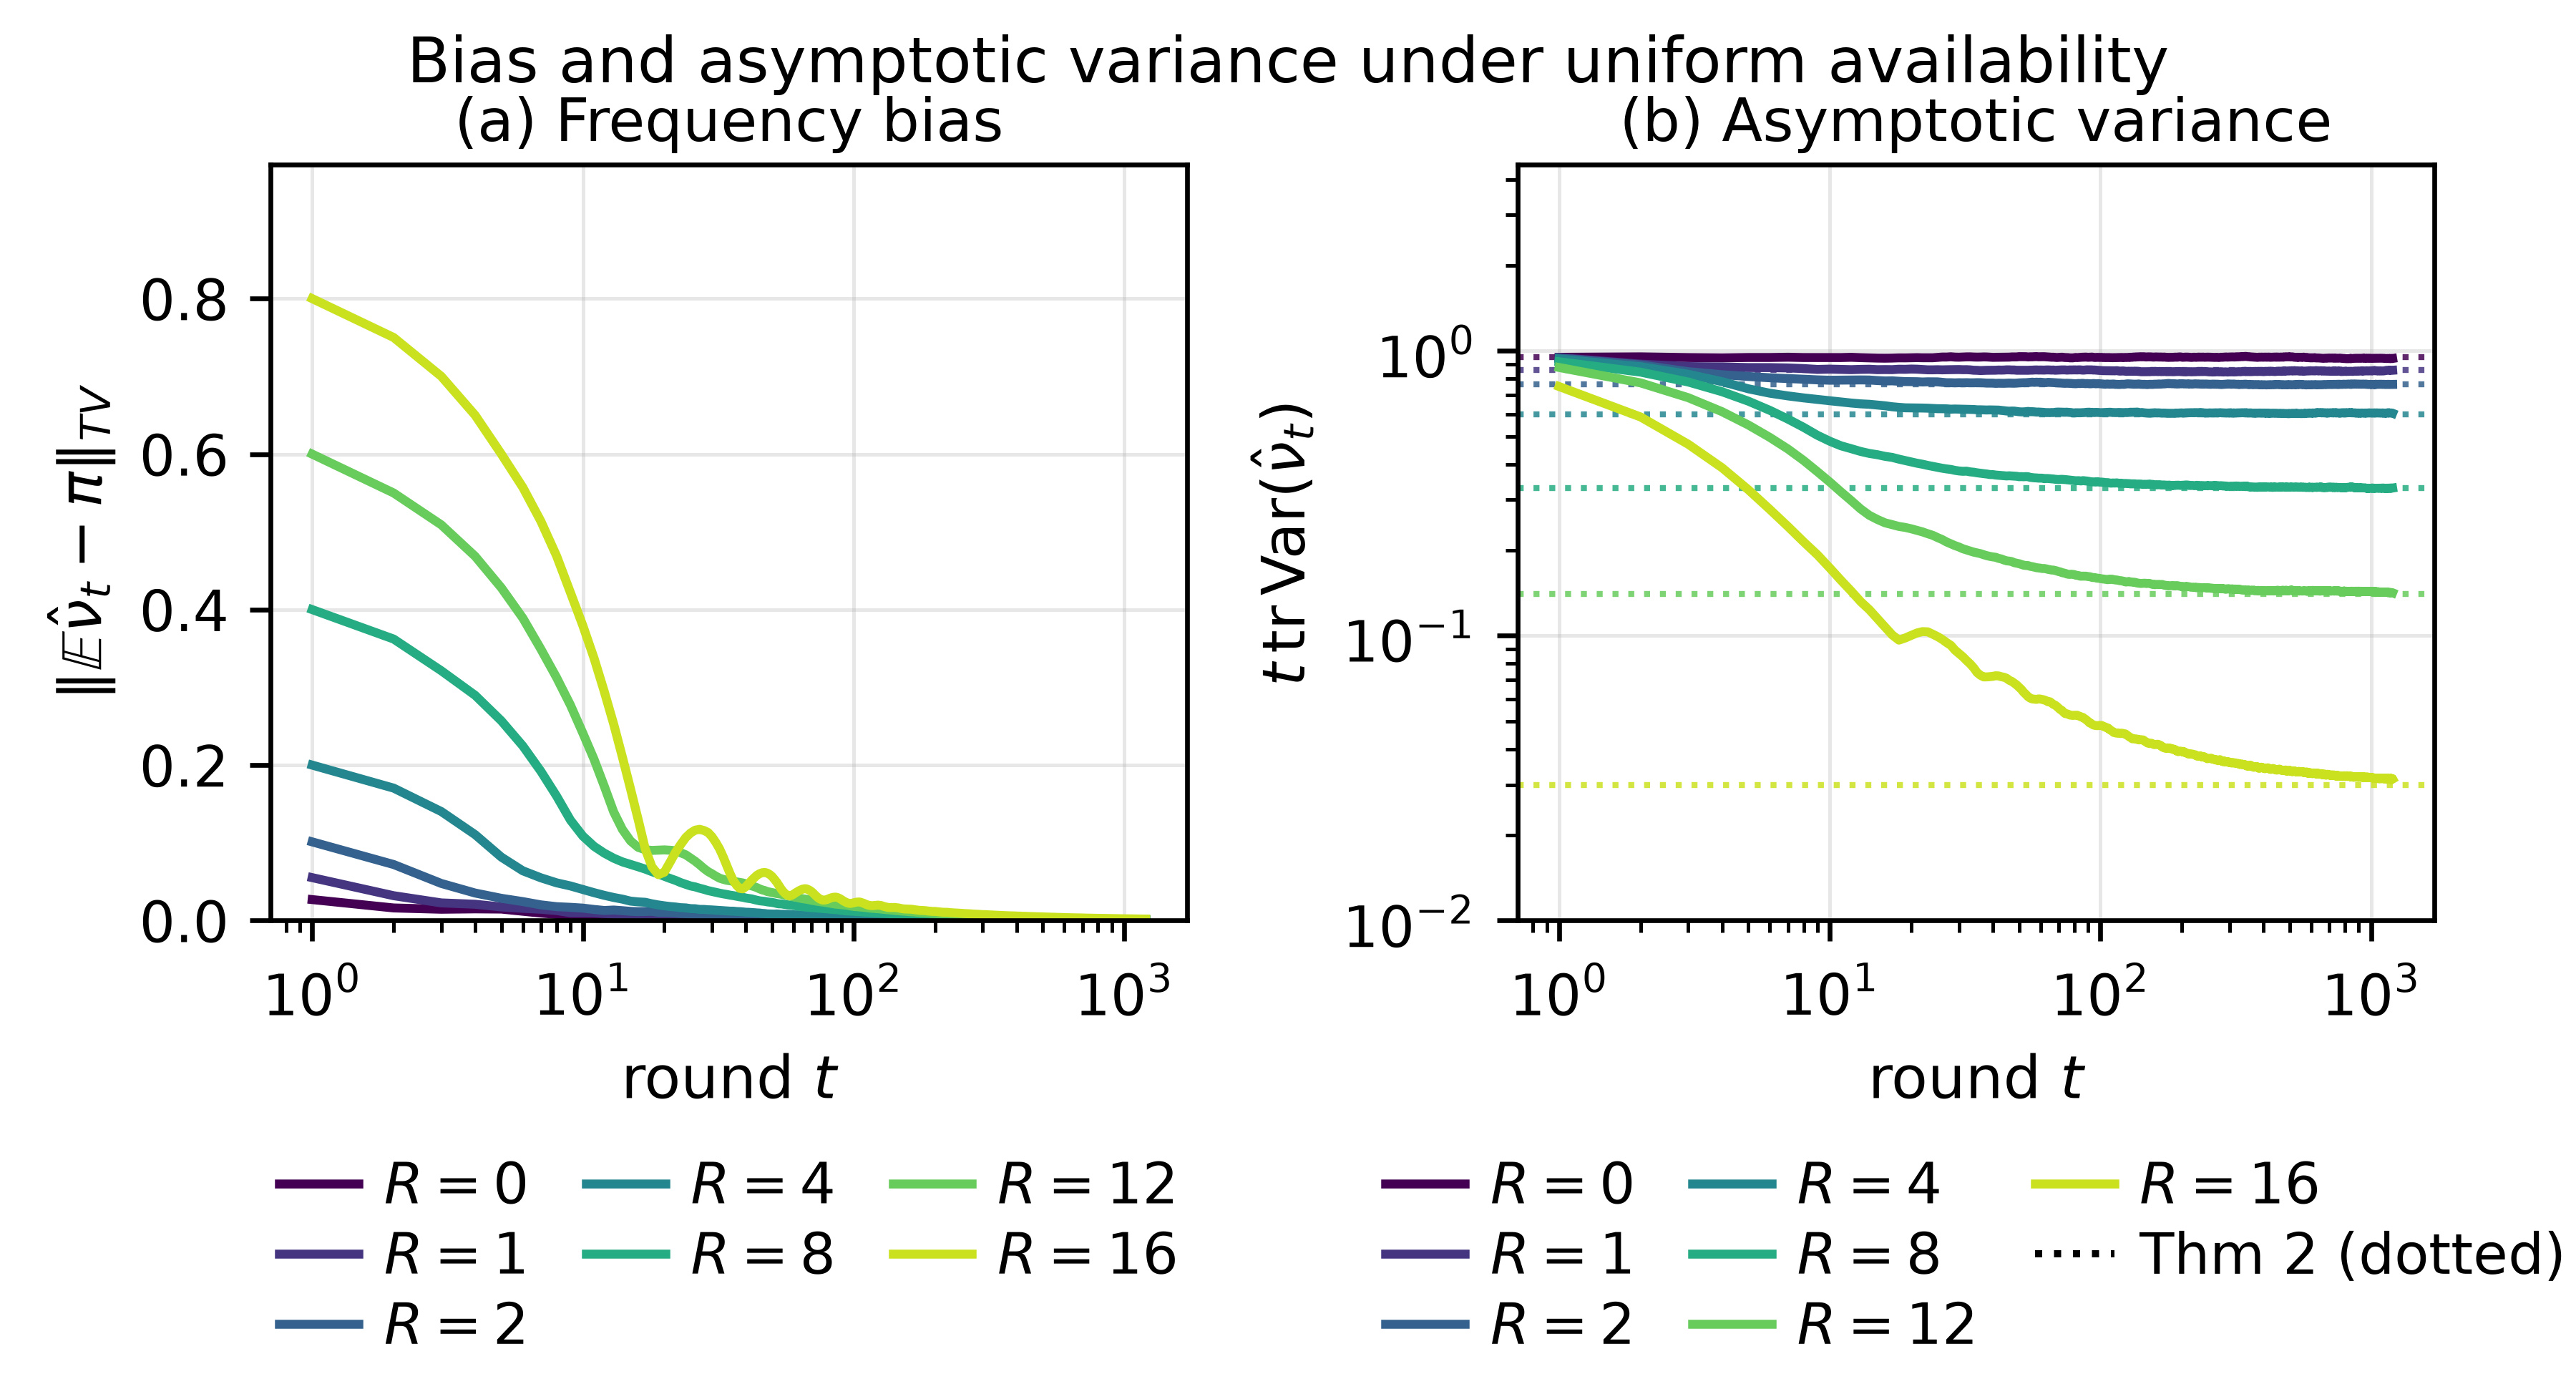
\includegraphics[width=\textwidth]{fig1.jpg}
\caption{Uniform availability with $N=20$ and $4000$ trajectories: (a) bias of the expected empirical frequency and (b) $t\,\mathrm{tr}\,\mathrm{Var}(\hat\nu_t)$ converging to $\sum_i\sigma_i^2(R)$ of Theorem 2 (dotted lines).}
\label{fig:1}
\vspace{2pt}
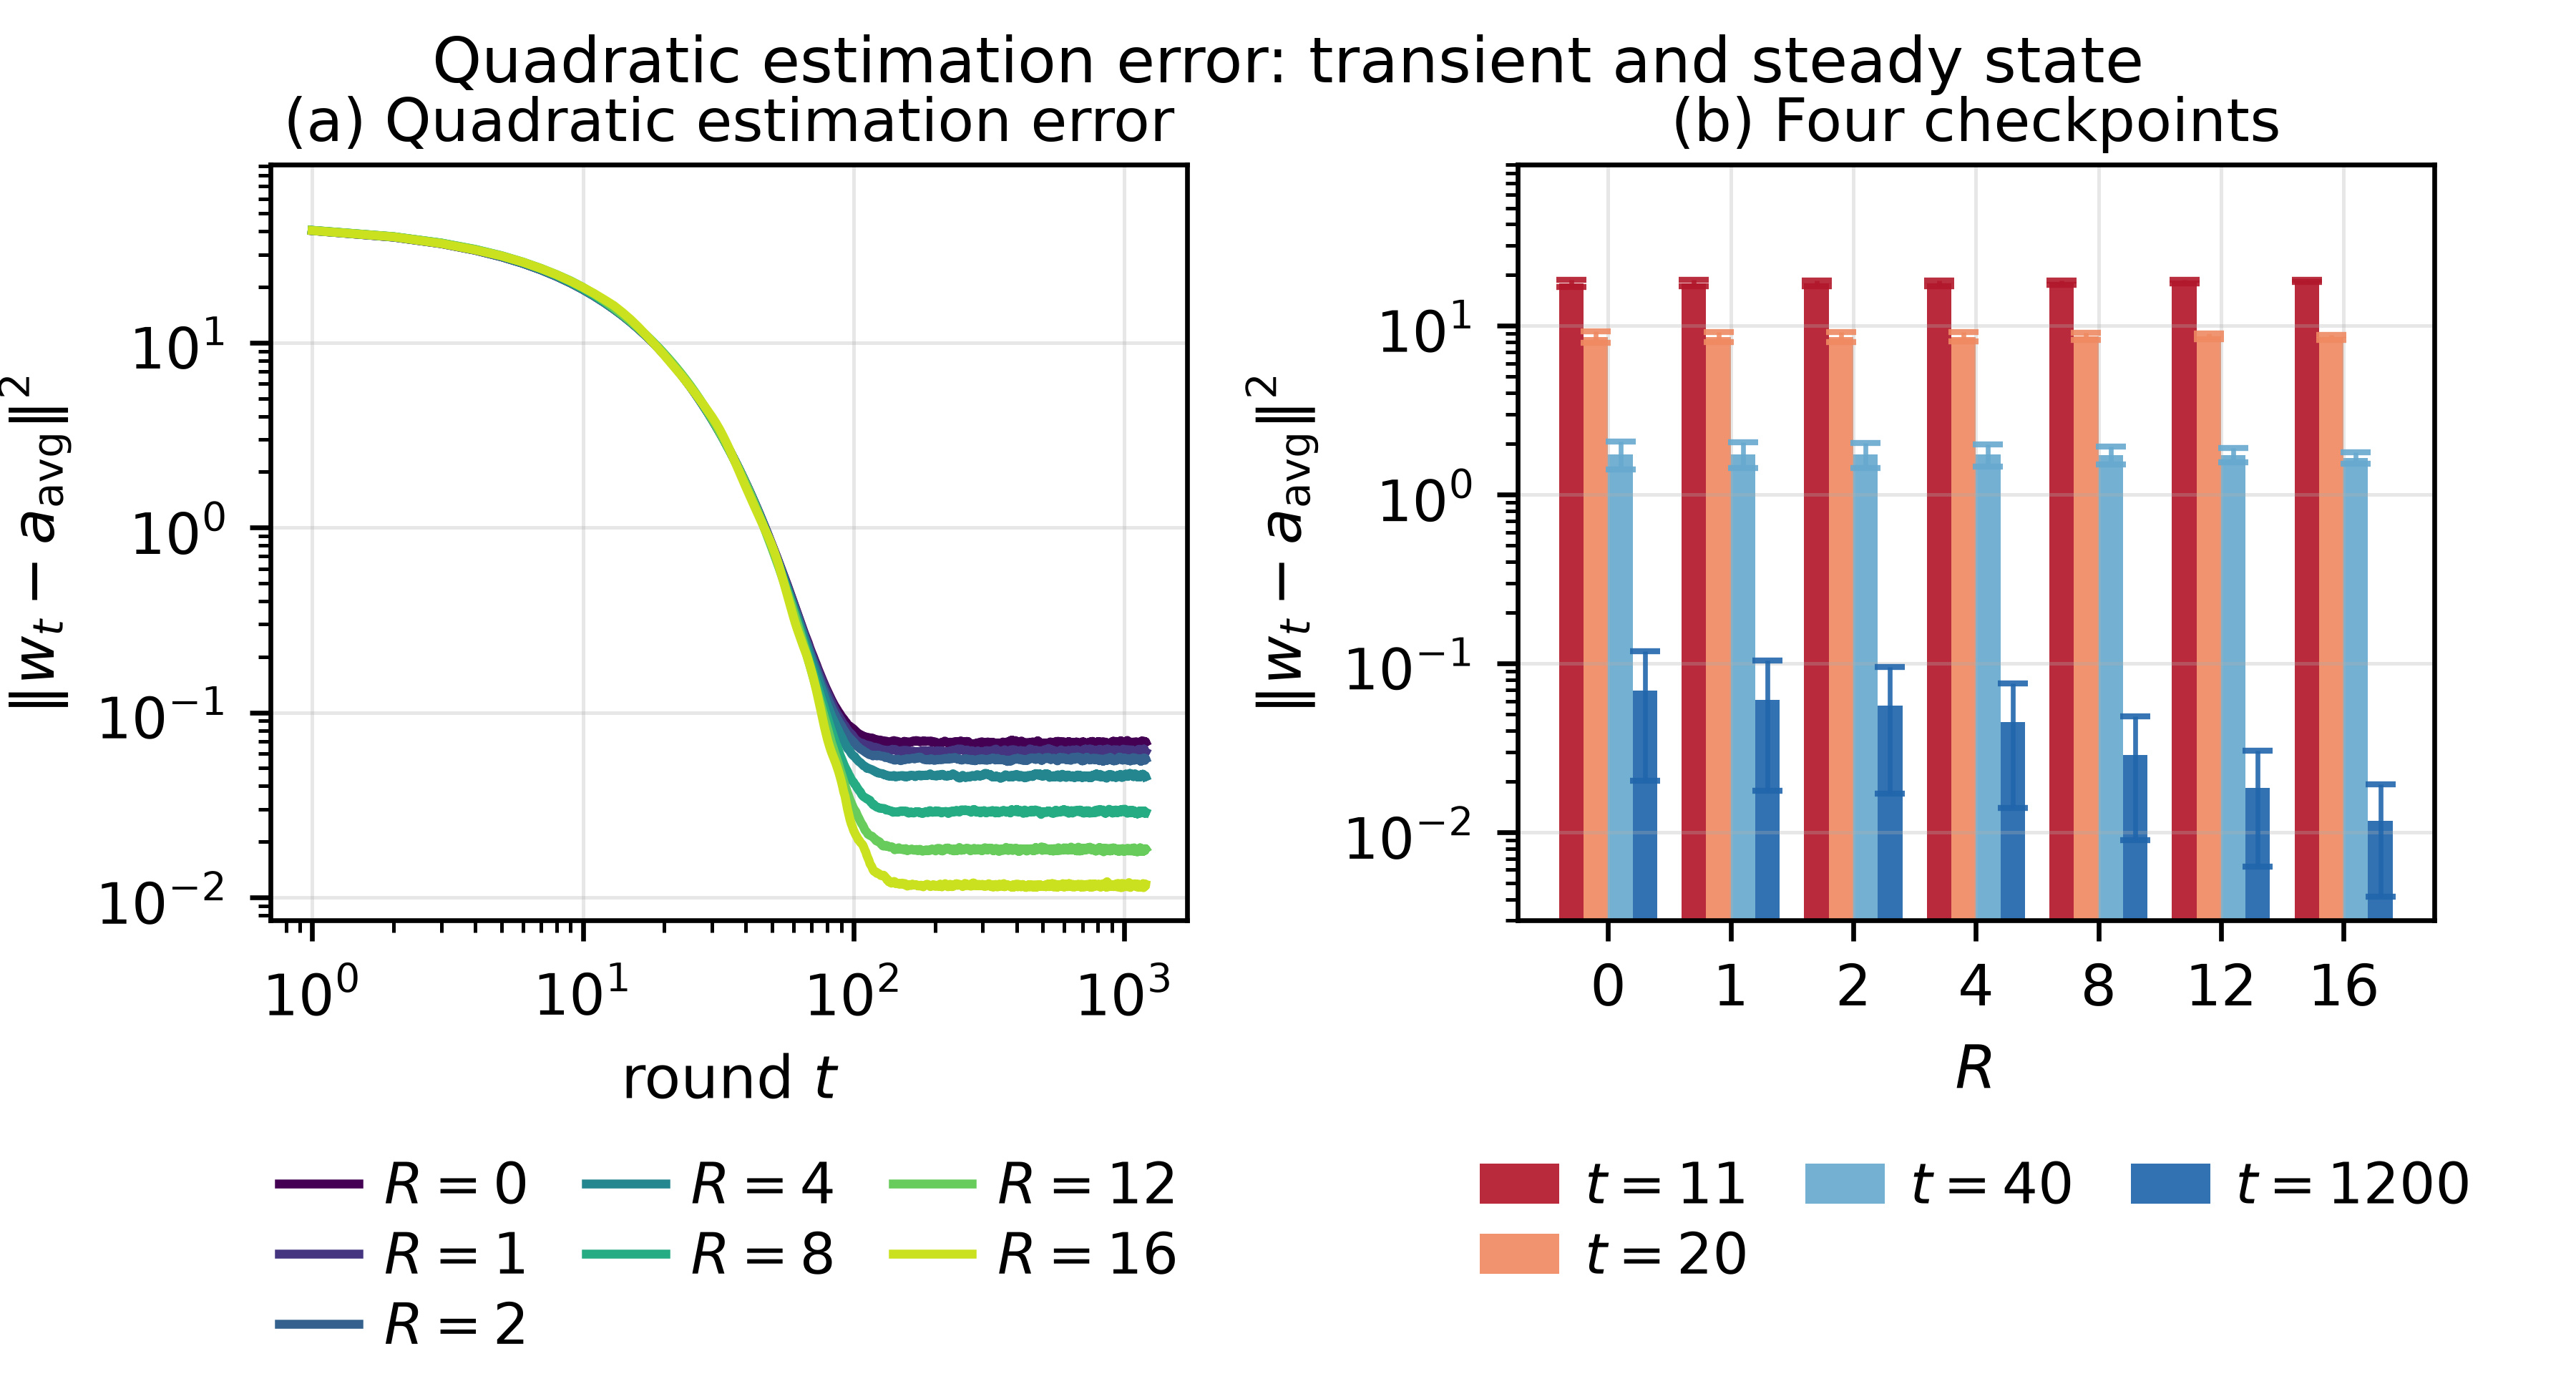
\includegraphics[width=\textwidth]{fig2.jpg}
\caption{Quadratic estimation error for $4000$ trajectories: (a) mean squared error versus round; (b) values at $t=11,20,40,1200$ on a logarithmic scale, with error bars of one standard deviation across trajectories.}
\label{fig:2}
\end{figure}

Fig.~\ref{fig:1}(a) shows $\|\mathbb{E}\hat\nu_t-\pi_R\|_{\mathrm{TV}}$,
whose value $R/N$ at $t=1$ is a deterministic-initialization artifact; for
$R=16$ it stays above $0.1$ until $t\approx17$. Panel (b) shows
$t\,\mathrm{tr\,Var}(\hat\nu_t)$ converging to
$\sum_i\sigma_i^{2}(R)=(N-R)(N-R-1)/N^{2}$ (dotted): at $t=1200$ all values
agree with Theorem 2 to within $5\%$, the largest deviation at $R=16$ being
transient bias rather than Monte Carlo error. No burn-in is applied here;
Fig.~\ref{fig:2}(b) error bars are one standard deviation.

Consider $N$ sensor nodes, node $k$ holding a vector observation $b_k\sim\mathcal{N}(0,\mathbf{I}_5)$, and a fusion center that at each round receives $b_{X_t}$ from the single admissible node and updates $w_{t+1}=(1-\eta)w_t+\eta b_{X_t}$ with $\eta=0.04$. Under uniform availability the stationary mean $\sum_i\pi_{R,i}b_i=N^{-1}\sum_k b_k$ is the population mean to be estimated, and $\mathbb{E}\|w_t-b_{\mathrm{avg}}\|^{2}$ is the steady-state estimation MSE; Proposition 3 gives it as an exponentially weighted covariance sum.

Fig.~\ref{fig:2} shows the steady-state error decreasing from
$0.0692$ at $R=0$ to $0.0117$ at $R=16$. At
$t=11$ a single data instance gives $+3.21\%$ for $R=16$ against $R=0$;
over $10$ independent sets of $\{b_k\}$ the difference has mean $-0.042$,
s.d. $0.522$, range $[-0.729,0.789]$ and no consistent sign, so the early
ordering is instance-dependent. The steady-state ratio $0.168\pm0.006$ is
below one in every repetition and matches the Proposition~4 closed form
$0.168944$ at $\eta=0.04$; it has the same direction as
$\sigma_i^{2}(R)$ but is not proportional, since Proposition 3 weights
covariances by $(1-\eta)^m$ while Theorem 2 uses the unweighted sum.
Proposition~3 reproduces the measured error to about $1\%$. The
unweighted limit $\eta\sigma_f^{2}/2$ gives $0.0679$ and $0.0021$ at $R=0,16$ against
$0.0692$ and $0.0117$; since $1-\lambda_\star(20,16)=0.0224<\eta$, the
zero-frequency constant lies outside its approximation regime and the
factor of about $5$ follows from the closed form.

\subsection{\texorpdfstring{Scope, non-uniform availability, and small-$\rho$ magnitude}{Scope, non-uniform availability, and small-rho magnitude}}
Theorem 2 covers uniform availability, under which the bias term of \citep[Thm.~1]{ref1} vanishes.

To examine aggregate variance outside the uniform case, we simulate
$p_i\propto i^{-1.5}$ with $N=100$ (client-level rather than the
group-level profile of \citep[Sec.~6]{ref1}), using $1200$ trajectories of
length $T=3000$ after a $600$-round burn-in; exact Poisson solves are
infeasible at $(100)_R$. At $R=0$ the estimate is $0.78908$ against the
analytic $0.79354$ ($0.56\%$ calibration error), decreasing monotonically to
$0.400$ at $R=20$ (Fig.~\ref{fig:3}). The skewed profile of Proposition 1
increases in aggregate from $0.0780$ to $0.3780$ at $R=0\to1$. Over
$20000$ Dirichlet$(\alpha_{\mathrm{Dir}})$ profiles the increase fraction is $17.1\%$ at
$N=5,\alpha_{\mathrm{Dir}}=0.2$, $0.56\%$ at $N=5,\alpha_{\mathrm{Dir}}=1$, and below $0.01\%$ for
$N\ge100$; the criterion is the closed-form inequality of Theorem~3.

\begin{figure}[!tp]
\centering
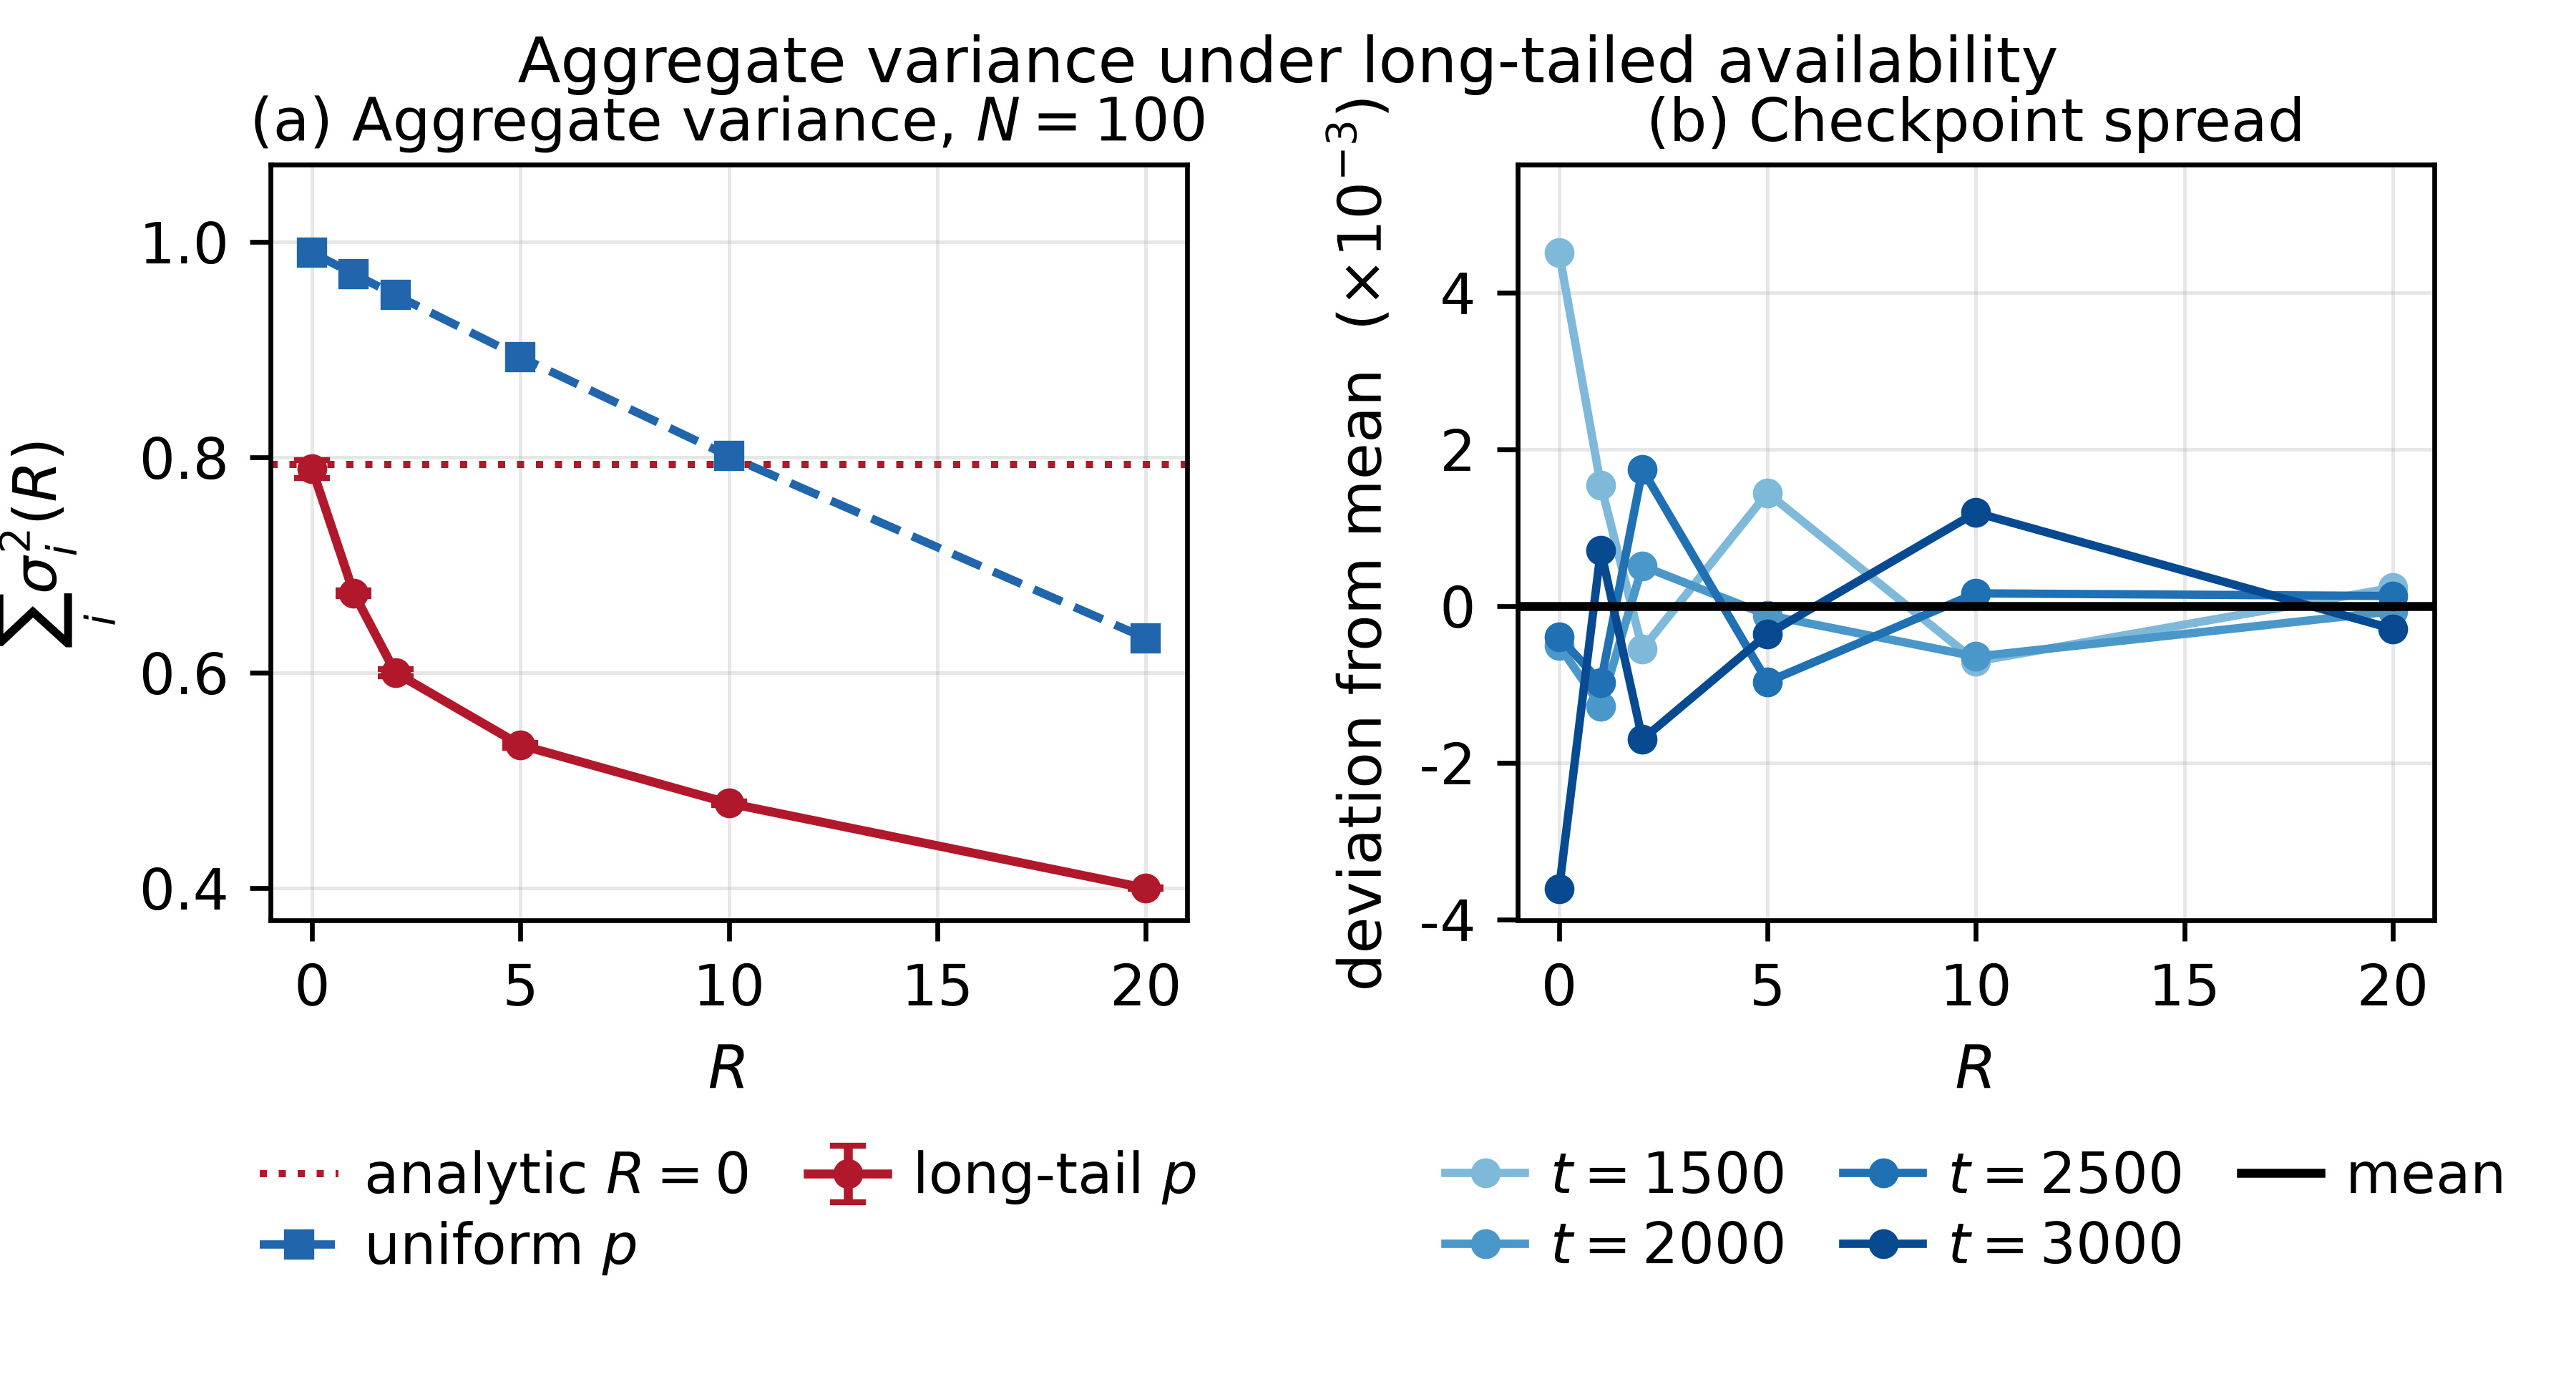
\includegraphics[width=\textwidth]{fig3.jpg}
\caption{Aggregate asymptotic variance $\sum_i\sigma_i^2(R)$ for $N=100$: (a) red, long-tailed $p_i\propto i^{-1.5}$ Monte Carlo with error bars giving the range over four checkpoints $t\in\{1500,2000,2500,3000\}$; blue dashed, uniform-availability closed form of Theorem 2 as a scale reference; red dotted, analytic $R=0$ calibration of the long-tailed model; (b) deviations of the four checkpoints from their mean, whose range supplies the error bars in (a).}
\label{fig:3}
\vspace{2pt}
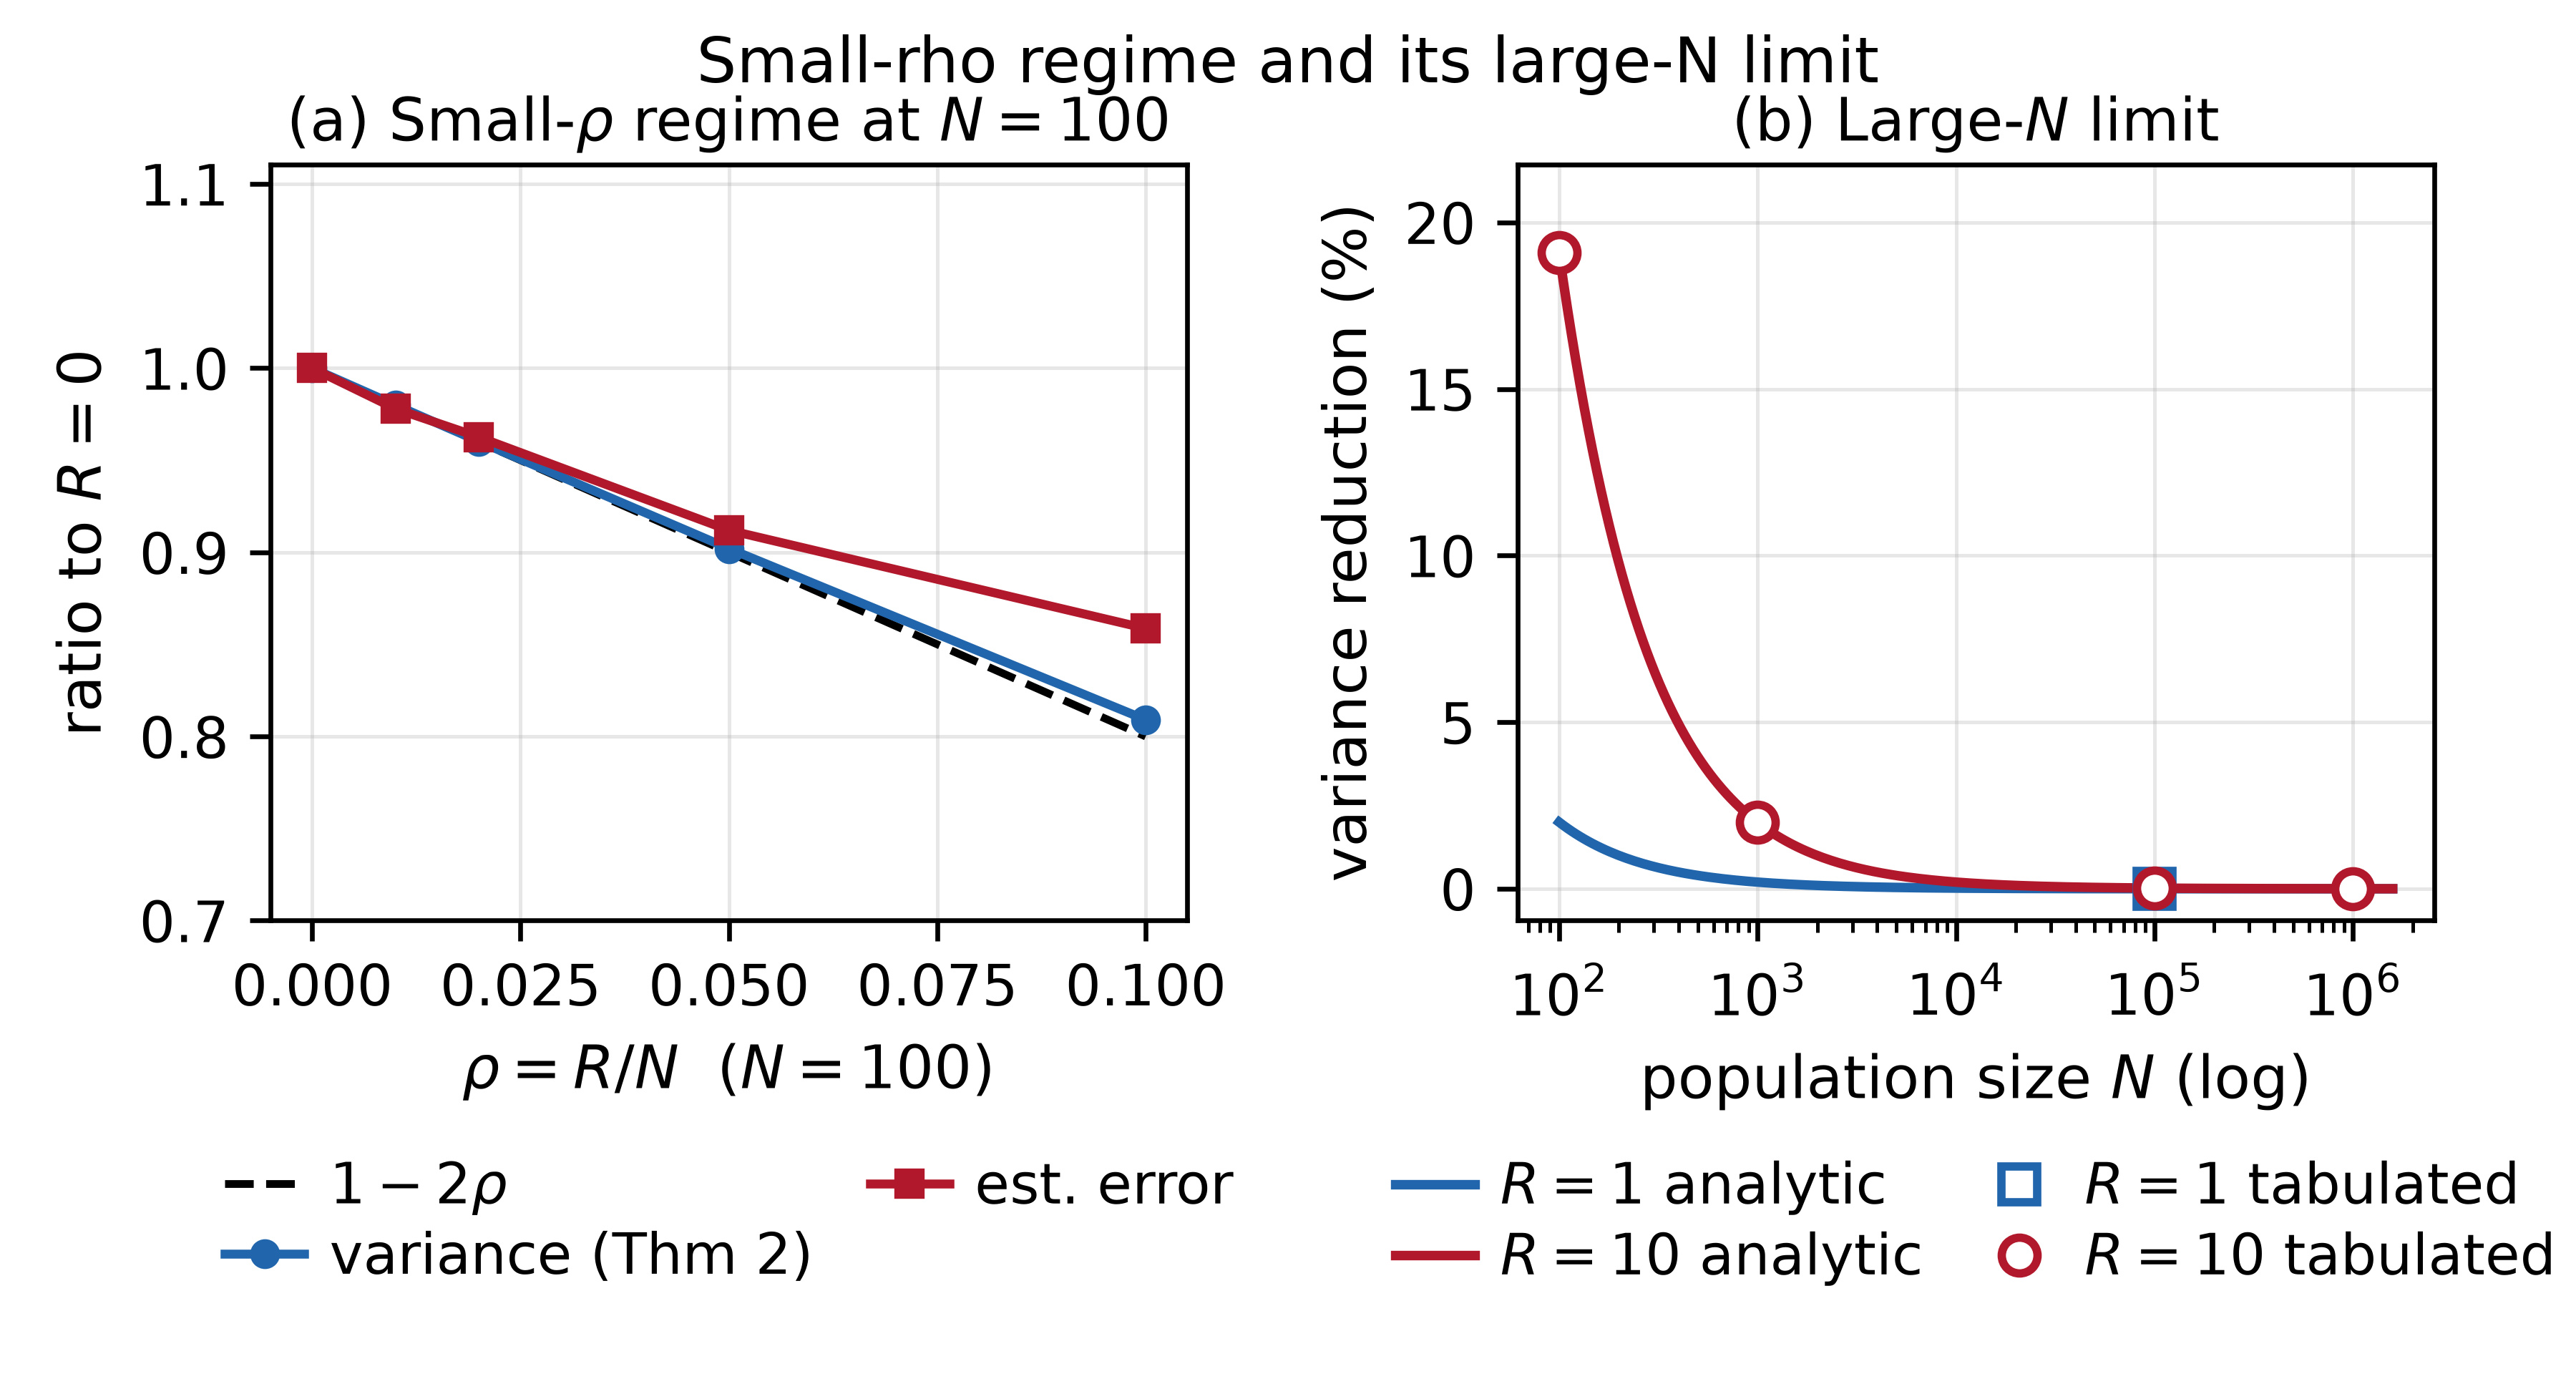
\includegraphics[width=\textwidth]{fig4.jpg}
\caption{Small-$\rho$ regime: (a) at $N=100$, the variance ratio of Theorem 2, the measured steady-state estimation-error ratio, and the asymptotic line $1-2\rho$; (b) the analytic variance reduction $100(1-\sum_i\sigma_i^2(R)/\sum_i\sigma_i^2(0))$ against population size $N$ for $R=1,10$, with the analytic values quoted in the text shown as markers.}
\label{fig:4}
\end{figure}

The magnitude of the effect depends on $\rho=R/N$. At $N=100$, $T=1200$, $2000$ trajectories and $\rho\in\{0,0.01,0.02,0.05,0.10\}$, the Theorem 2 variance ratio follows $1-2\rho$ to within about one percent, whereas the measured steady-state error ratio is about seven percent above it at $\rho=0.10$ (Fig.~\ref{fig:4}). At $N=10^{5},R=10$ the closed form gives a relative variance reduction of $0.0200\%$, and $0.0020\%$ at $R=1$.

\subsection{Spectral Certificates and Design Rules}
\textbf{E1 --- prefactor certificate at $N=100$.} This population size
matches the long-tail experiment of Section~6.3 and the client profile of
E5. The lumped chain has $D_R$ states independently of $N$, so exact
iteration remains feasible up to $R\le7$. Table~\ref{table:IV} lists the exact $\tau_{\mathrm{mix}}$, $C(q)$
and \eqref{eq:e28}; every row has slack, and $\tau_{\mathrm{mix}}\ge R$ is
attained for $R\le6$. Fig.~\ref{fig:5}(a) gives the fully exact $N=10$ case;
panel (b) extends to the provable bound and $R+L$ for larger $R$.

\begin{figure}[!tp]
\centering
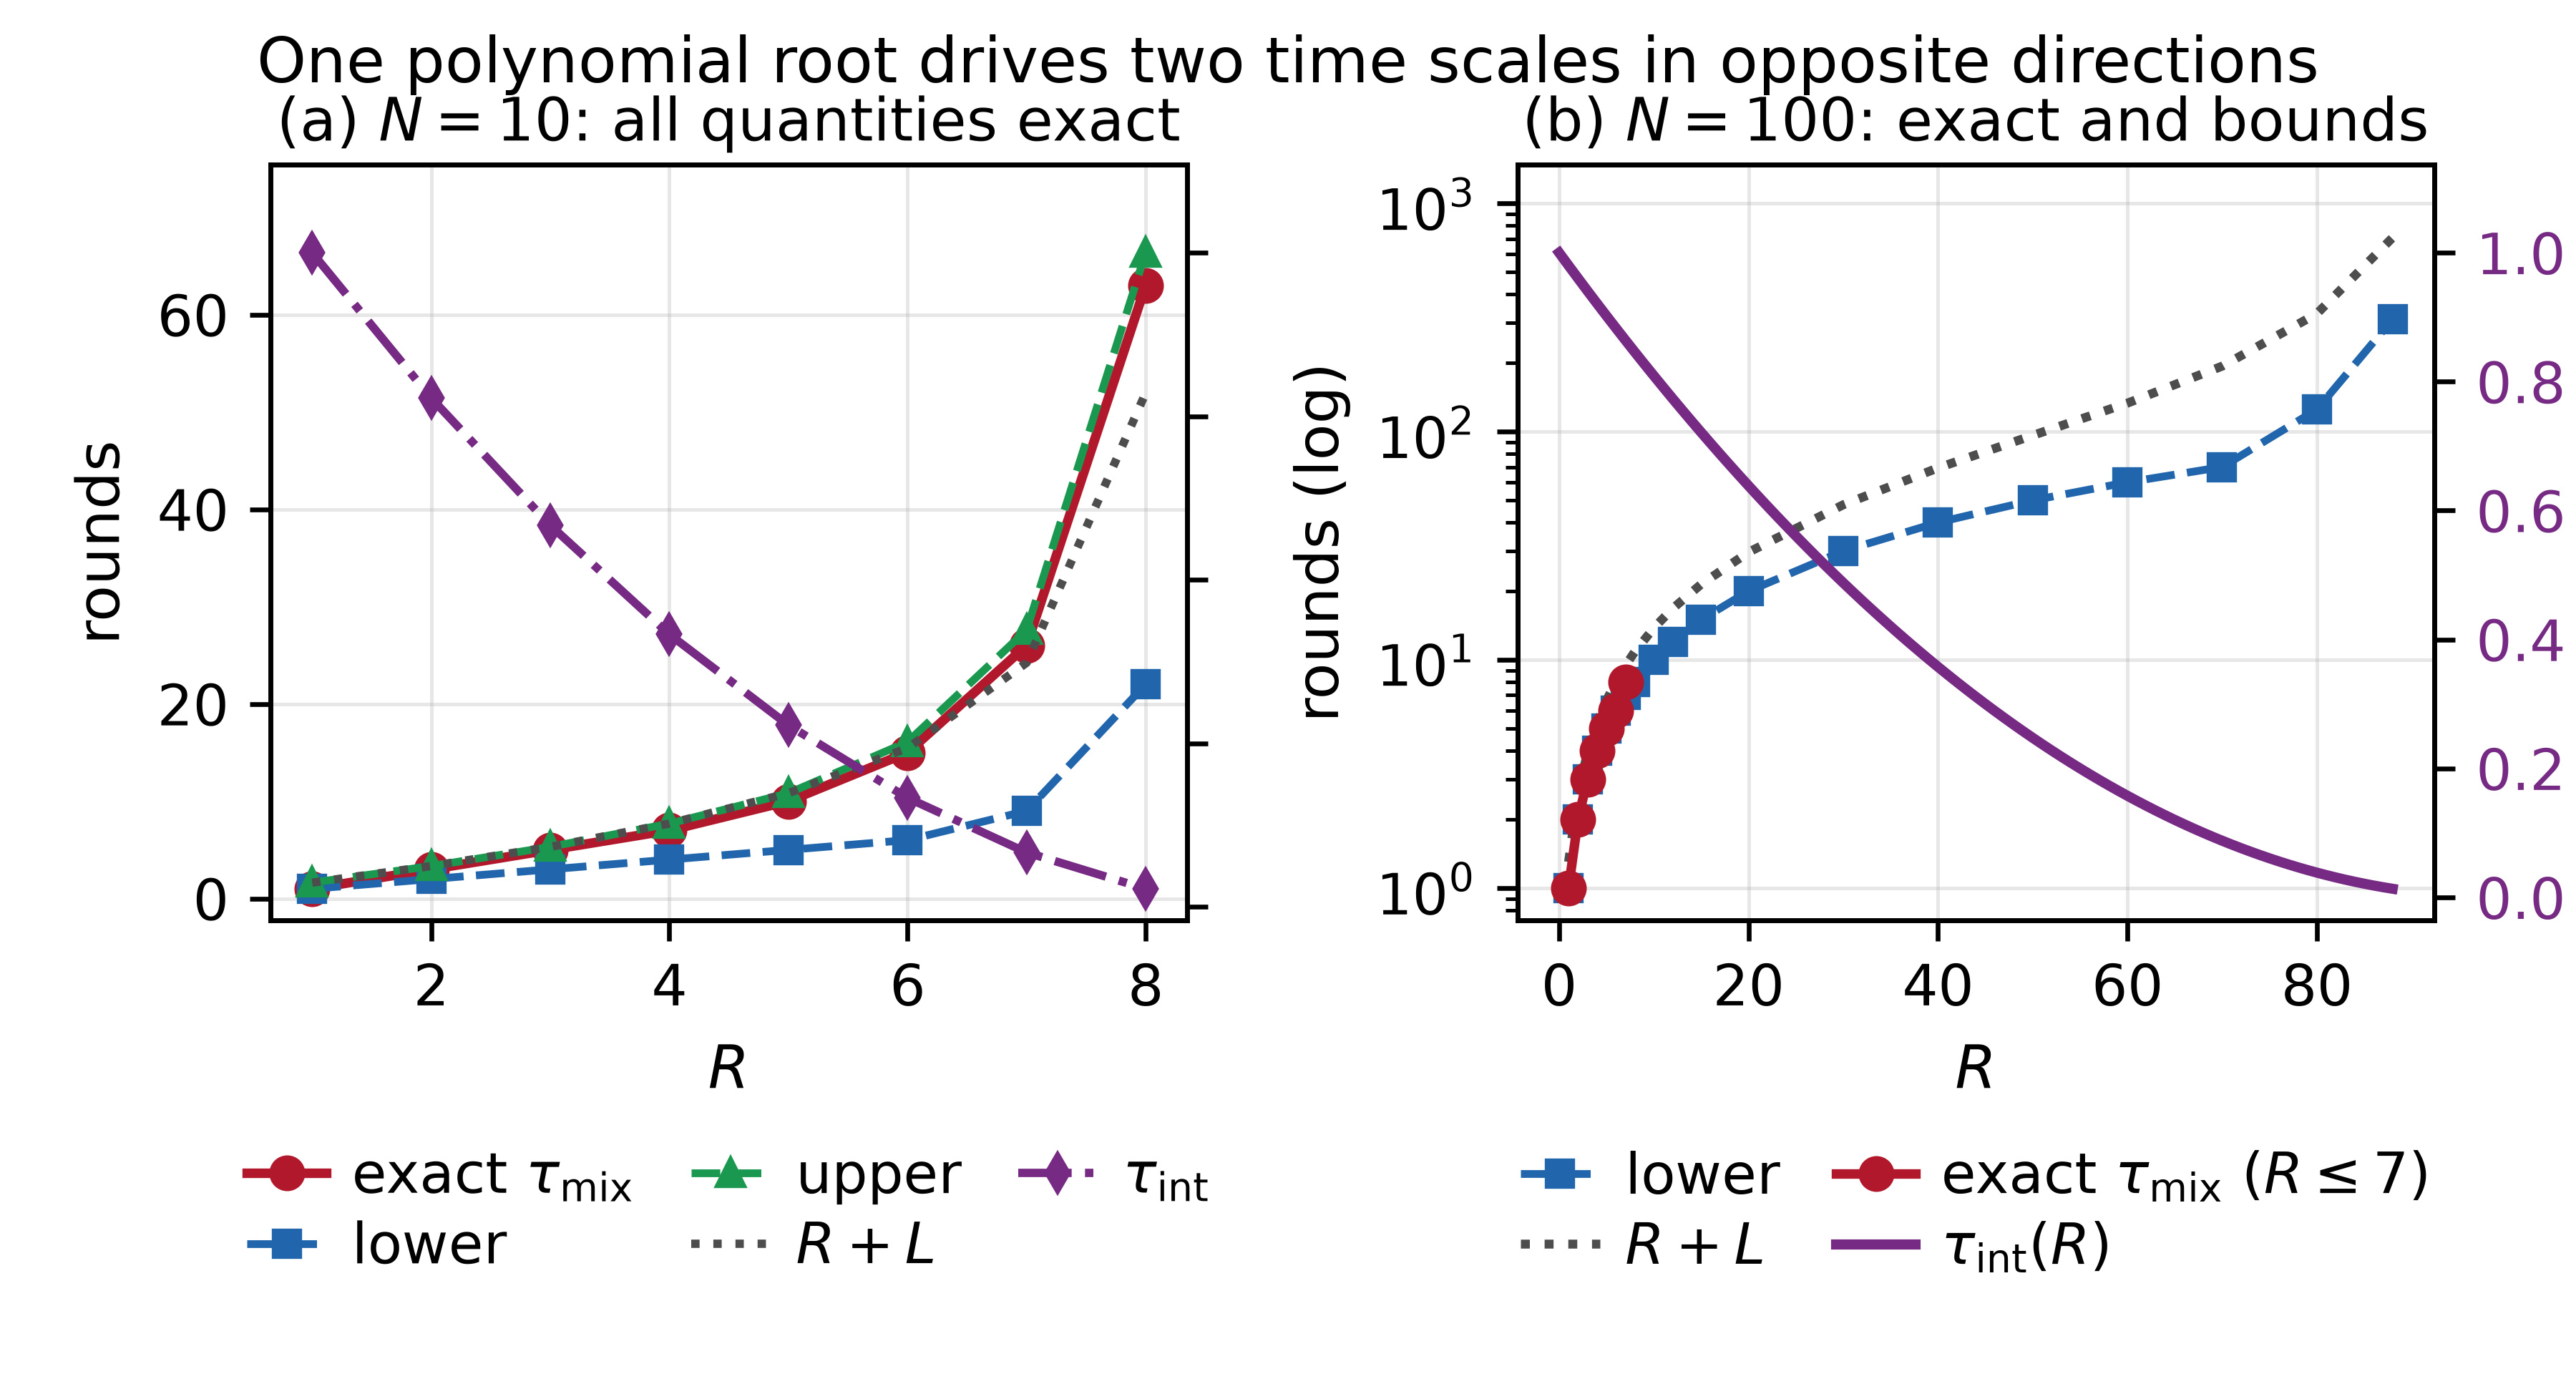
\includegraphics[width=\textwidth]{fig5.jpg}
\caption{One polynomial root drives two time scales in opposite directions.
(a) $N=10$, all quantities exact: $\tau_{\mathrm{mix}}$ grows while
$\tau_{\mathrm{int}}$ (right axis, linear) falls. (b) $N=100$: exact
$\tau_{\mathrm{mix}}$ for $R\leq7$ and the provable lower bound plus the
leading term $R+L$ (left axis, log) for larger $R$; $\tau_{\mathrm{int}}(R)$
(right axis, linear) is the closed form of Theorem 2.}
\label{fig:5}
\vspace{2pt}
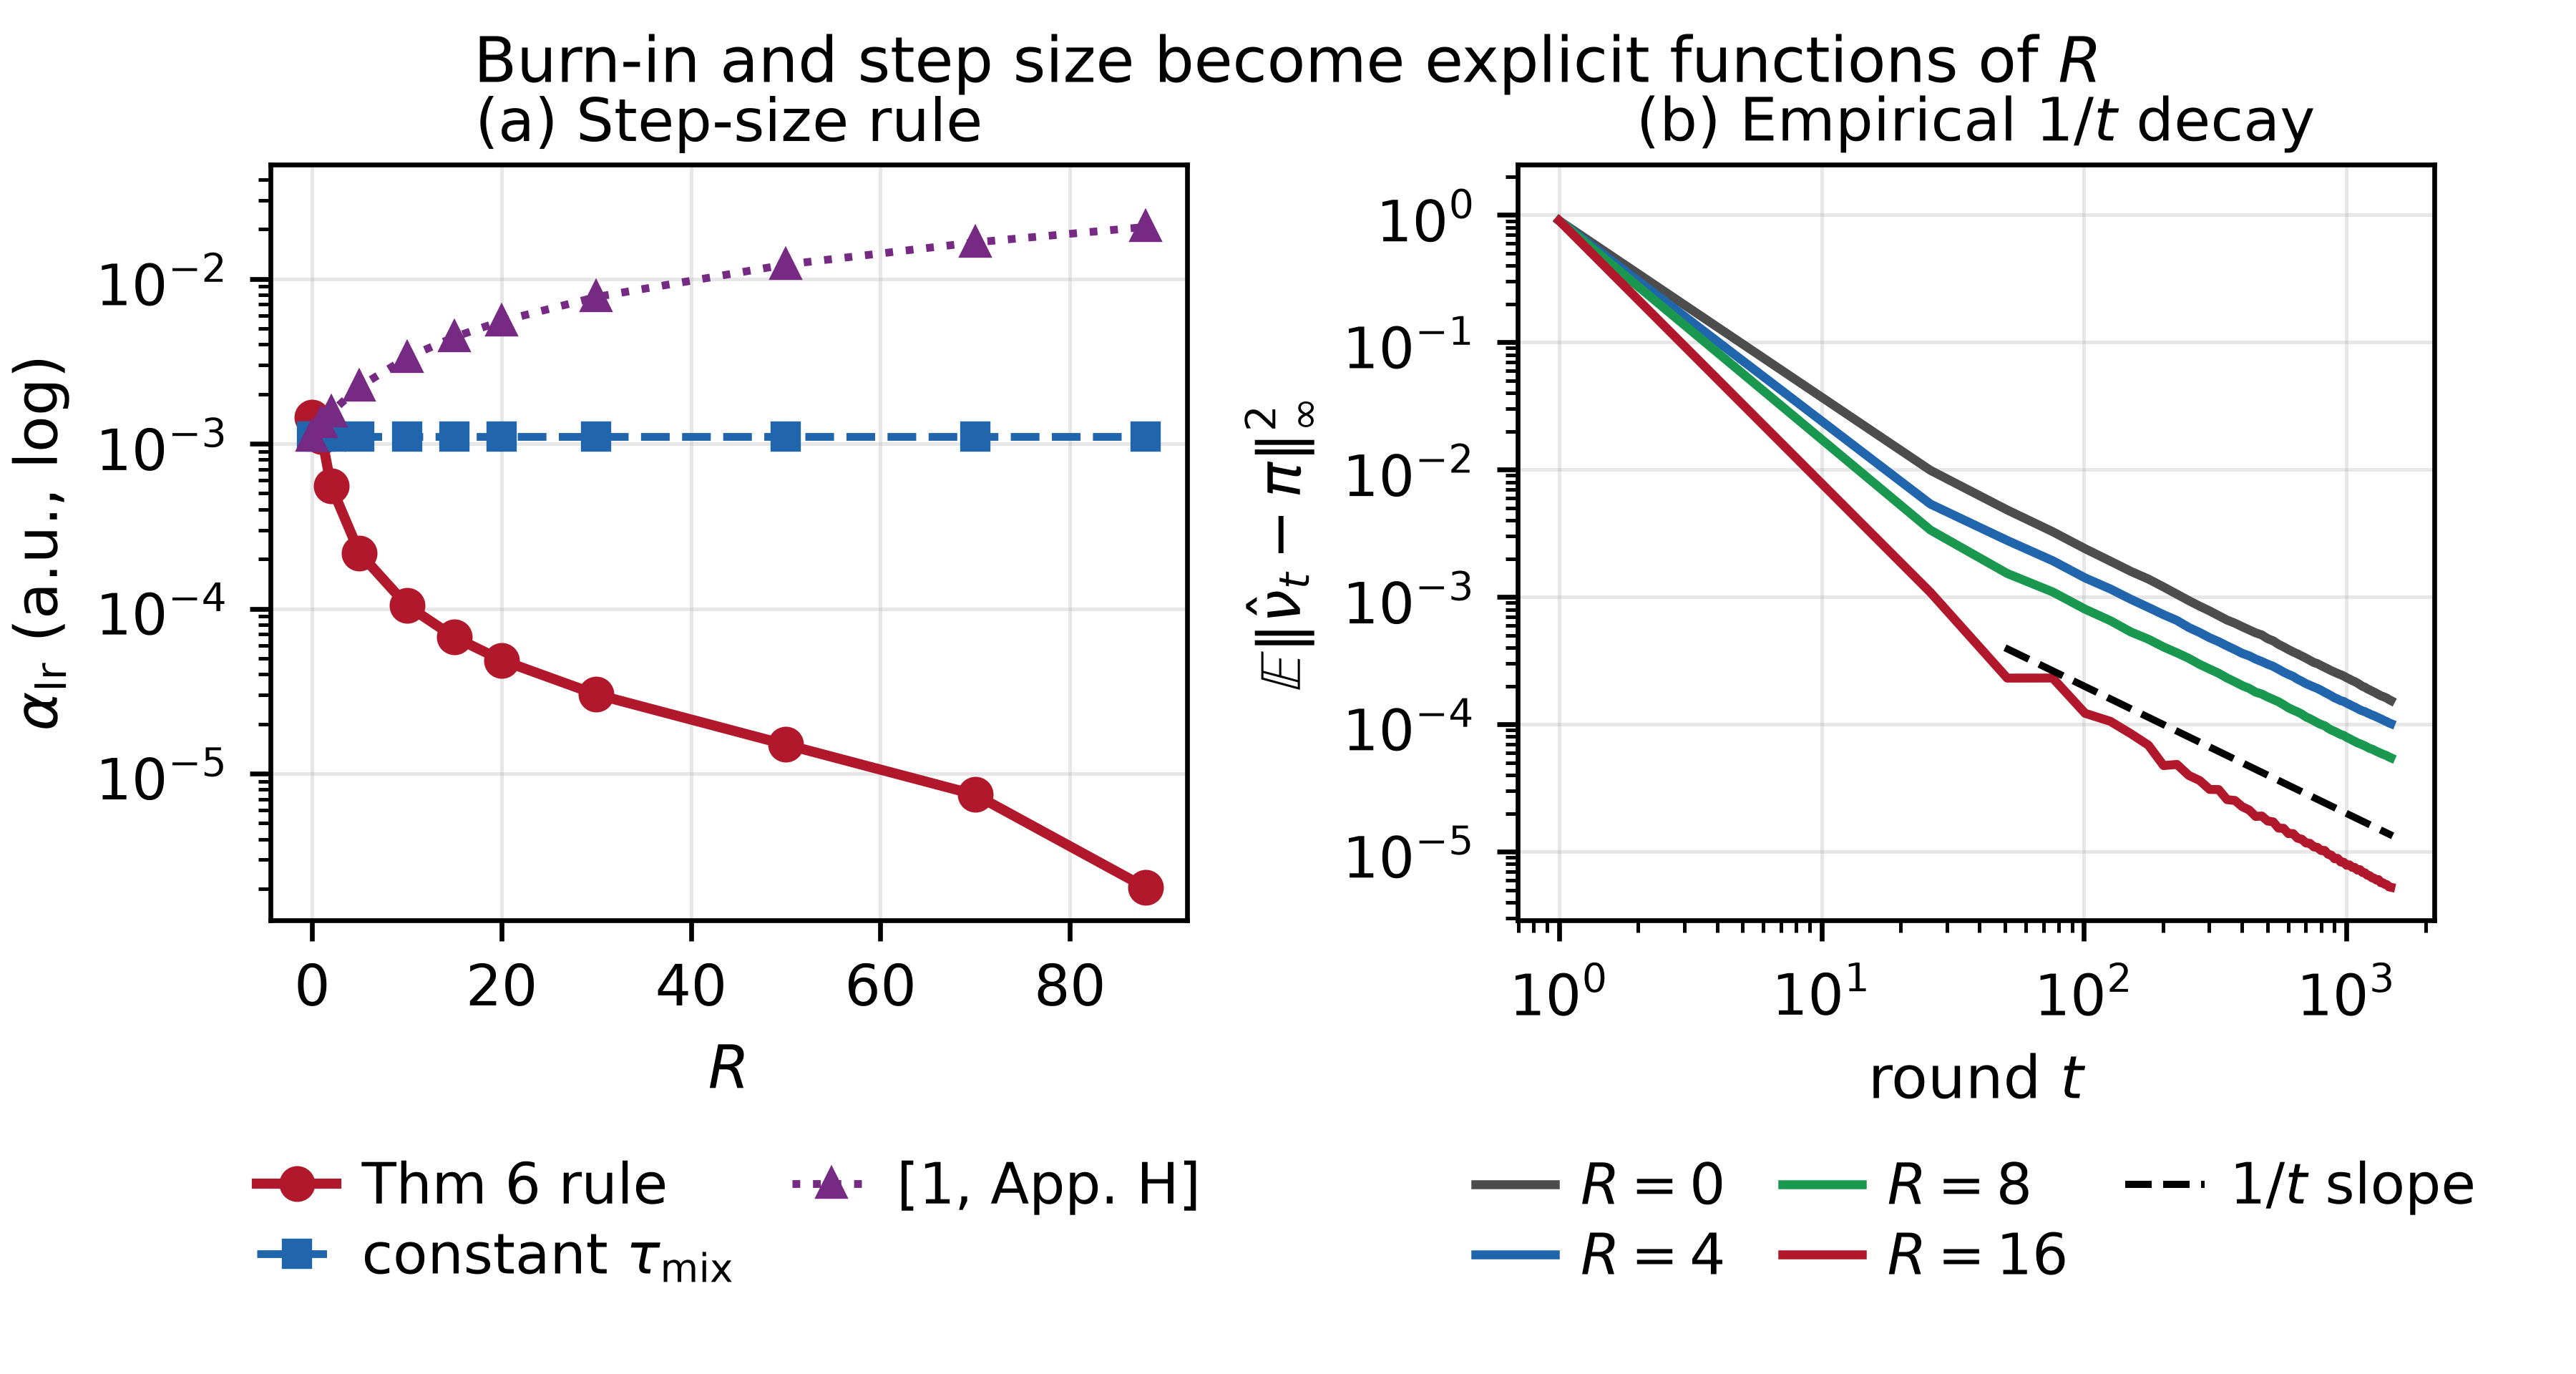
\includegraphics[width=\textwidth]{fig6.jpg}
\caption{(a) Step-size rule from Theorem 6 versus a constant-$\tau_{\mathrm{mix}}$
baseline and a schematic of the decreasing-$\tau_{\mathrm{mix}}$ conjecture in
\protect\citep[App.~H]{ref1}. (b) Empirical concentration on a $1/t$ slope; the kink
of $R=16$ near $t\approx70$ is the transient caused by the deterministic cooldown release,
not sampling noise. The magnitude falls with $R$, for which $R+L$ equals $1.0$, $6.2$,
$14.5$, $77.1$ at $R=0,4,8,16$, respectively.}
\label{fig:6}
\end{figure}

\begin{table}[!t]
\small
\centering
\begin{tabular}{@{}ccccccc@{}}
\toprule
$R$ & $\lambda_\star$ & $L$ & $\tau_{\mathrm{mix}}$ & $R+L$ & $C(q)$ & upper \\
\midrule
1 & 0.01010 & 0.30 & 1 & 1.30 & 0.010 & 1.30 \\
2 & 0.10102 & 0.60 & 2 & 2.60 & 0.099 & 2.60 \\
3 & 0.22419 & 0.93 & 3 & 3.93 & 0.199 & 3.93 \\
4 & 0.33645 & 1.27 & 4 & 5.27 & 0.288 & 5.27 \\
5 & 0.42957 & 1.64 & 5 & 6.64 & 0.377 & 6.64 \\
6 & 0.50520 & 2.03 & 6 & 8.03 & 0.463 & 8.03 \\
7 & 0.56670 & 2.44 & 8 & 9.44 & 0.575 & 9.44 \\
\bottomrule
\end{tabular}
\caption{Exact prefactor certificate at $N=100$ (E1). $L=\ln4/|\ln\lambda_\star|$,
$C(q)=\sup_{s\geq1}d(R+s)/\lambda_\star^{s}$; the last column is \eqref{eq:e28}.}
\label{table:IV}
\end{table}

\textbf{E2 --- step size and burn-in.} Theorem~6 makes
$\alpha_{\mathrm{lr}}=\widetilde{\mathcal{O}}(1/(\tau_{\mathrm{mix}}K\sqrt T))$
and $T>2\tau_{\mathrm{mix}}\log\tau_{\mathrm{mix}}$ explicit in $R$. With
$N=100$, $T=1200$, $K=20$ and $\tau_{\mathrm{mix}}\approx R+L$, the rule gives
$\alpha_{\mathrm{lr}}=1.11\times10^{-3}$ at $R=1$ and
$2.04\times10^{-6}$ at $R=88$ against a constant-$\tau_{\mathrm{mix}}$
baseline of $1.11\times10^{-3}$ (a factor of $544$); the burn-in grows from
$3$ to $9.3\times10^{3}$ rounds. Fig.~\ref{fig:6}(a) plots the Theorem~6 rule against two reference curves:
a constant-$\tau_{\mathrm{mix}}$ baseline and the decreasing-$\tau_{\mathrm{mix}}$
trend conjectured in \citep[App.~H]{ref1}, shown for visual comparison only
and not used in any bound. Panel (b) uses $1000$ trajectories to display the
$1/t$ decay.

\textbf{Remark 7.} In Fig.~\ref{fig:6}(b),
$t\,\mathbb{E}\|\hat\nu_t-\pi_R\|_\infty^{2}$ equals $0.228$, $0.149$,
$0.080$, $0.0078$ at $R=0,4,8,16$ and decreases with $R$, following
$\tau_{\mathrm{int}}(R)$ (the concentration bound
$\mathcal{O}(\tau_{\mathrm{mix}}/t)$ of \citep[Lemma~2]{ref1} concerns
$\mathbb{E}\|\tilde\nu_t\|_\infty^2$, a different object, and instead
grows with $R$ because $\tau_{\mathrm{mix}}(R)\ge R$ by Theorem~1).

\textbf{E3 --- finite step size.} Proposition~4 agrees with an
independent truncated covariance recursion to
$3.0\times10^{-13}$; at $(N,R,\eta)=(20,16,0.04)$ the closed form gives
$0.168944262$, matching the measured $0.168\pm0.006$ of Section~6.2.
Fig.~\ref{fig:7}(a) shows the zero-frequency constant and the boundary
$\eta=1-\lambda_\star$; (b) shows the finite-$\eta$ error exceeding the
zero-frequency prediction once $\eta>1-\lambda_\star$. At $\eta=0.04$
and $1-\lambda_\star(20,16)=0.0224$ the Poisson kernel of width
$\Theta(\eta)$ exceeds the distance to the nearest covariance
singularity, so the zero-frequency constant $0.0021$ is replaced by the full closed form
$0.0117$, a factor of about $5$.

\begin{figure}[!tp]
\centering
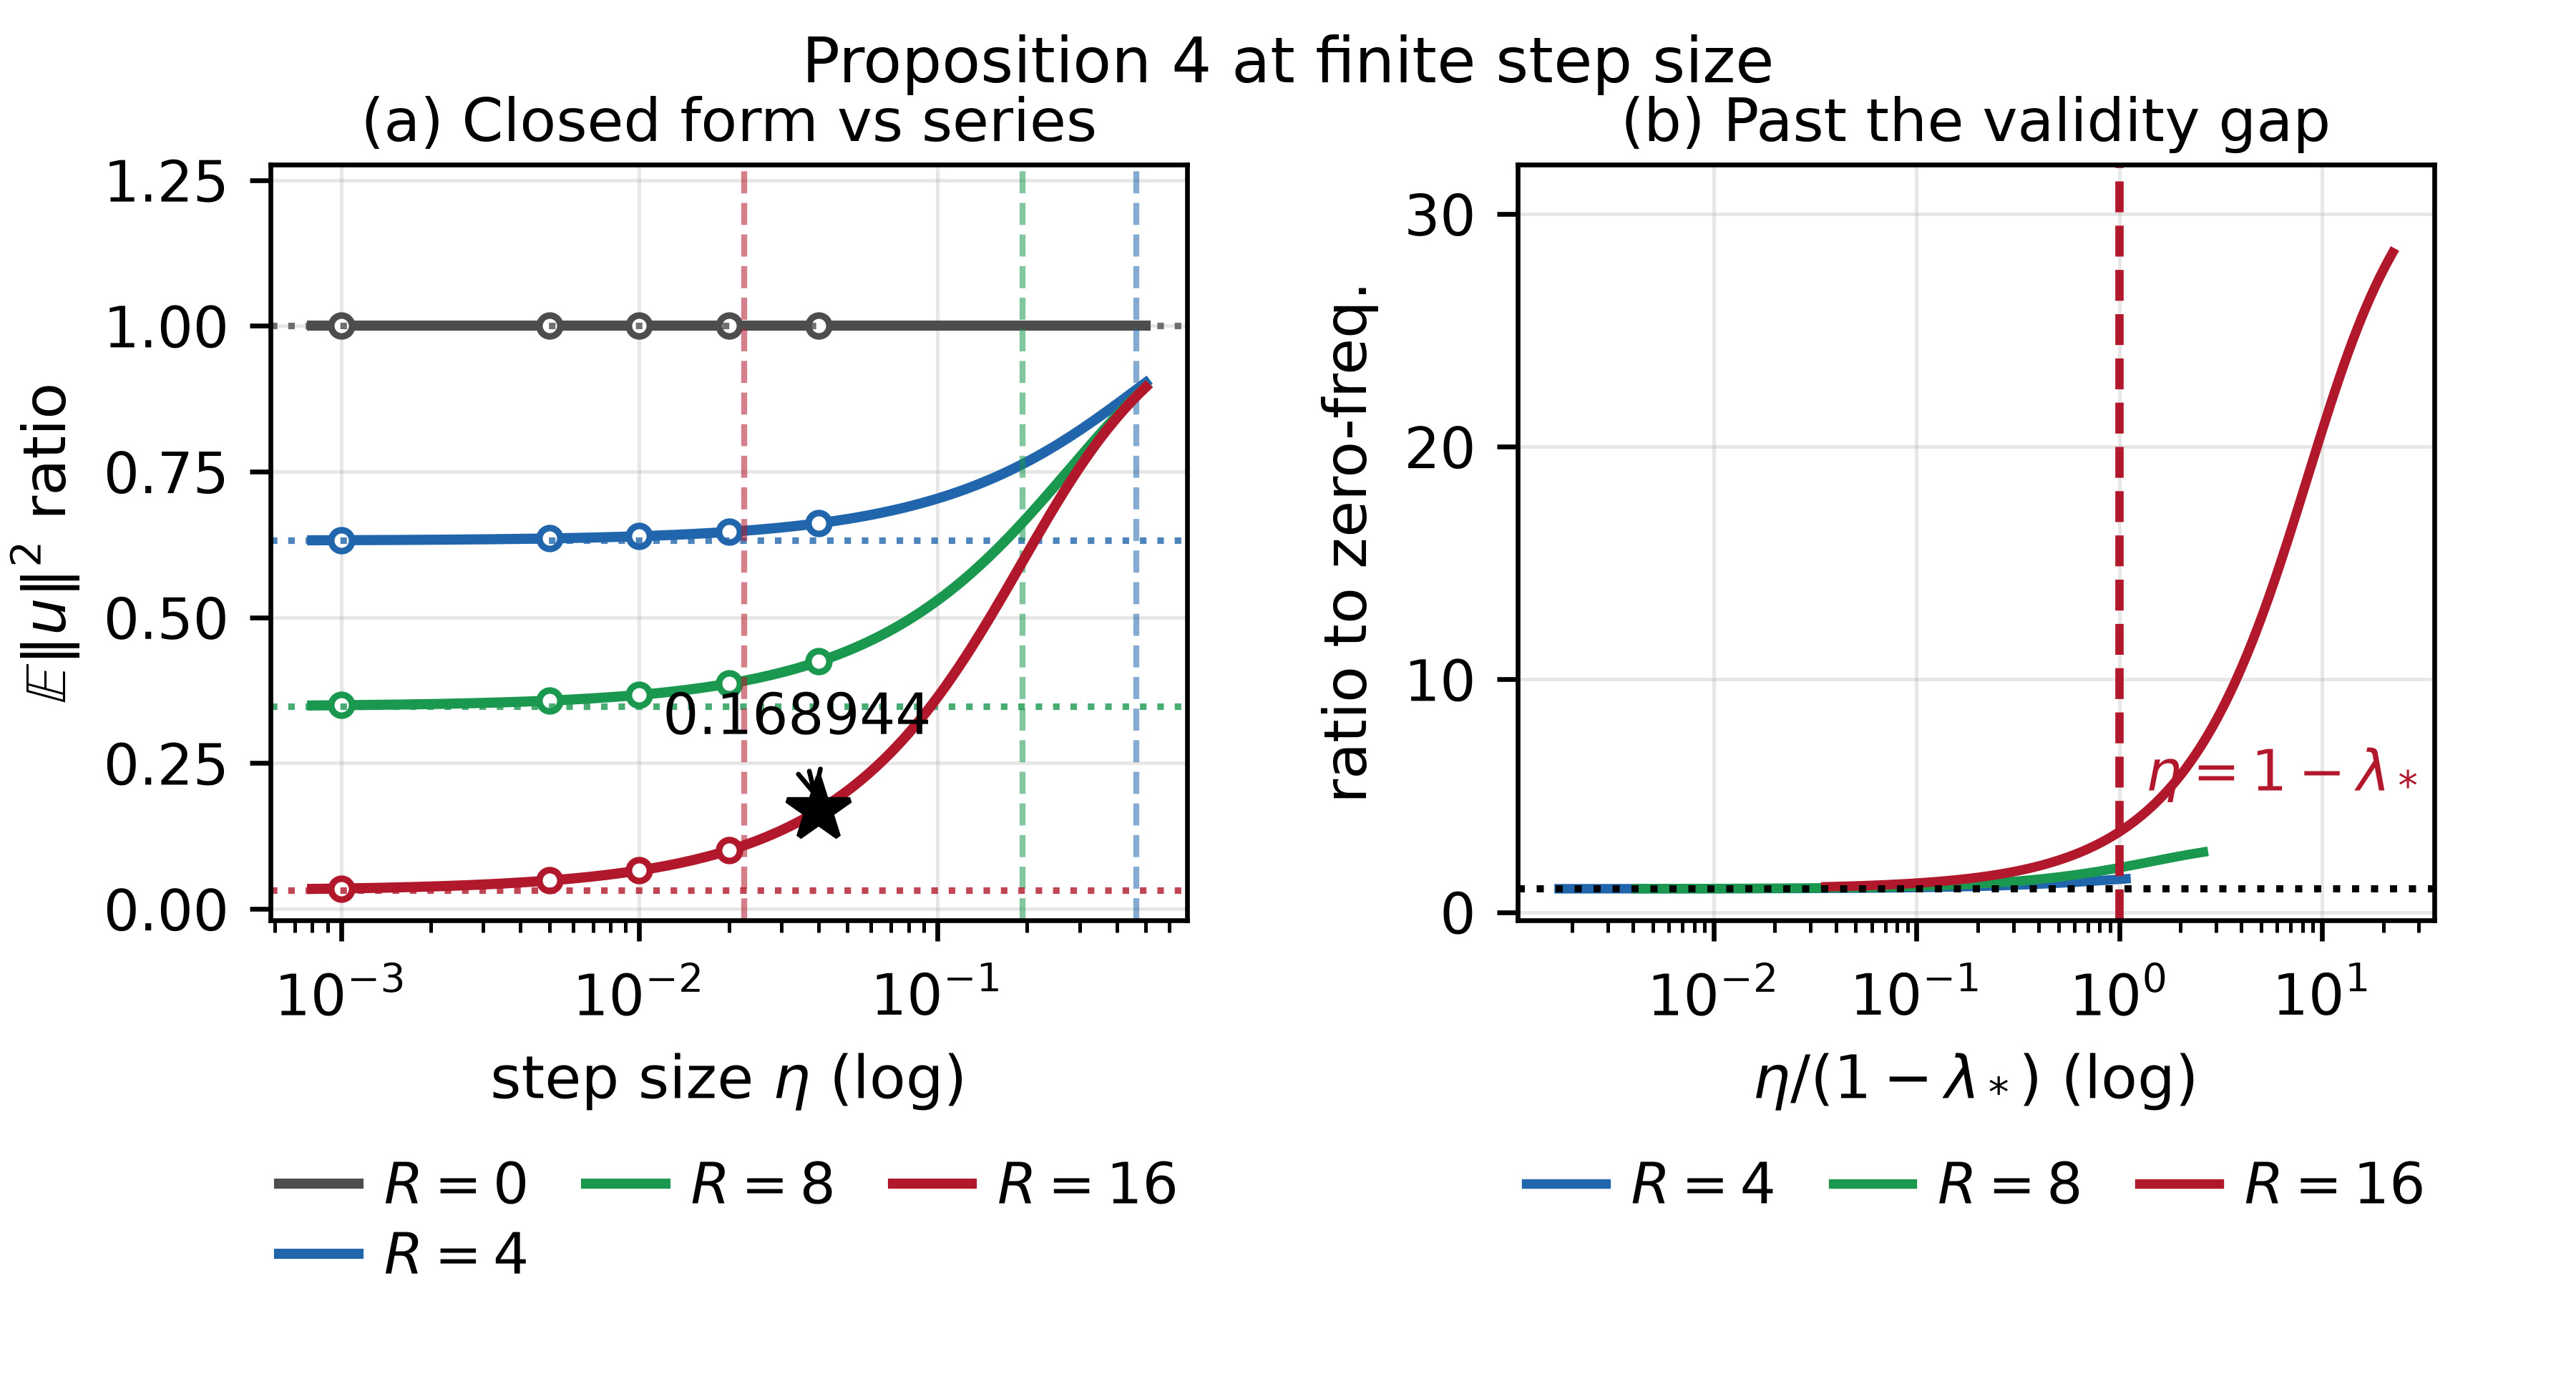
\includegraphics[width=\textwidth]{fig7.jpg}
\caption{Proposition 4 at finite step size. (a) Closed form (lines) versus the
independent truncated covariance series (circles), with zero-frequency
levels (dotted) and the boundaries $\eta=1-\lambda_\star$ (dashed); the star
marks $0.168944$ at $(N,R,\eta)=(20,16,0.04)$. (b) Ratio of the finite-$\eta$
error to the zero-frequency prediction against $\eta/(1-\lambda_\star)$.}
\label{fig:7}
\vspace{2pt}
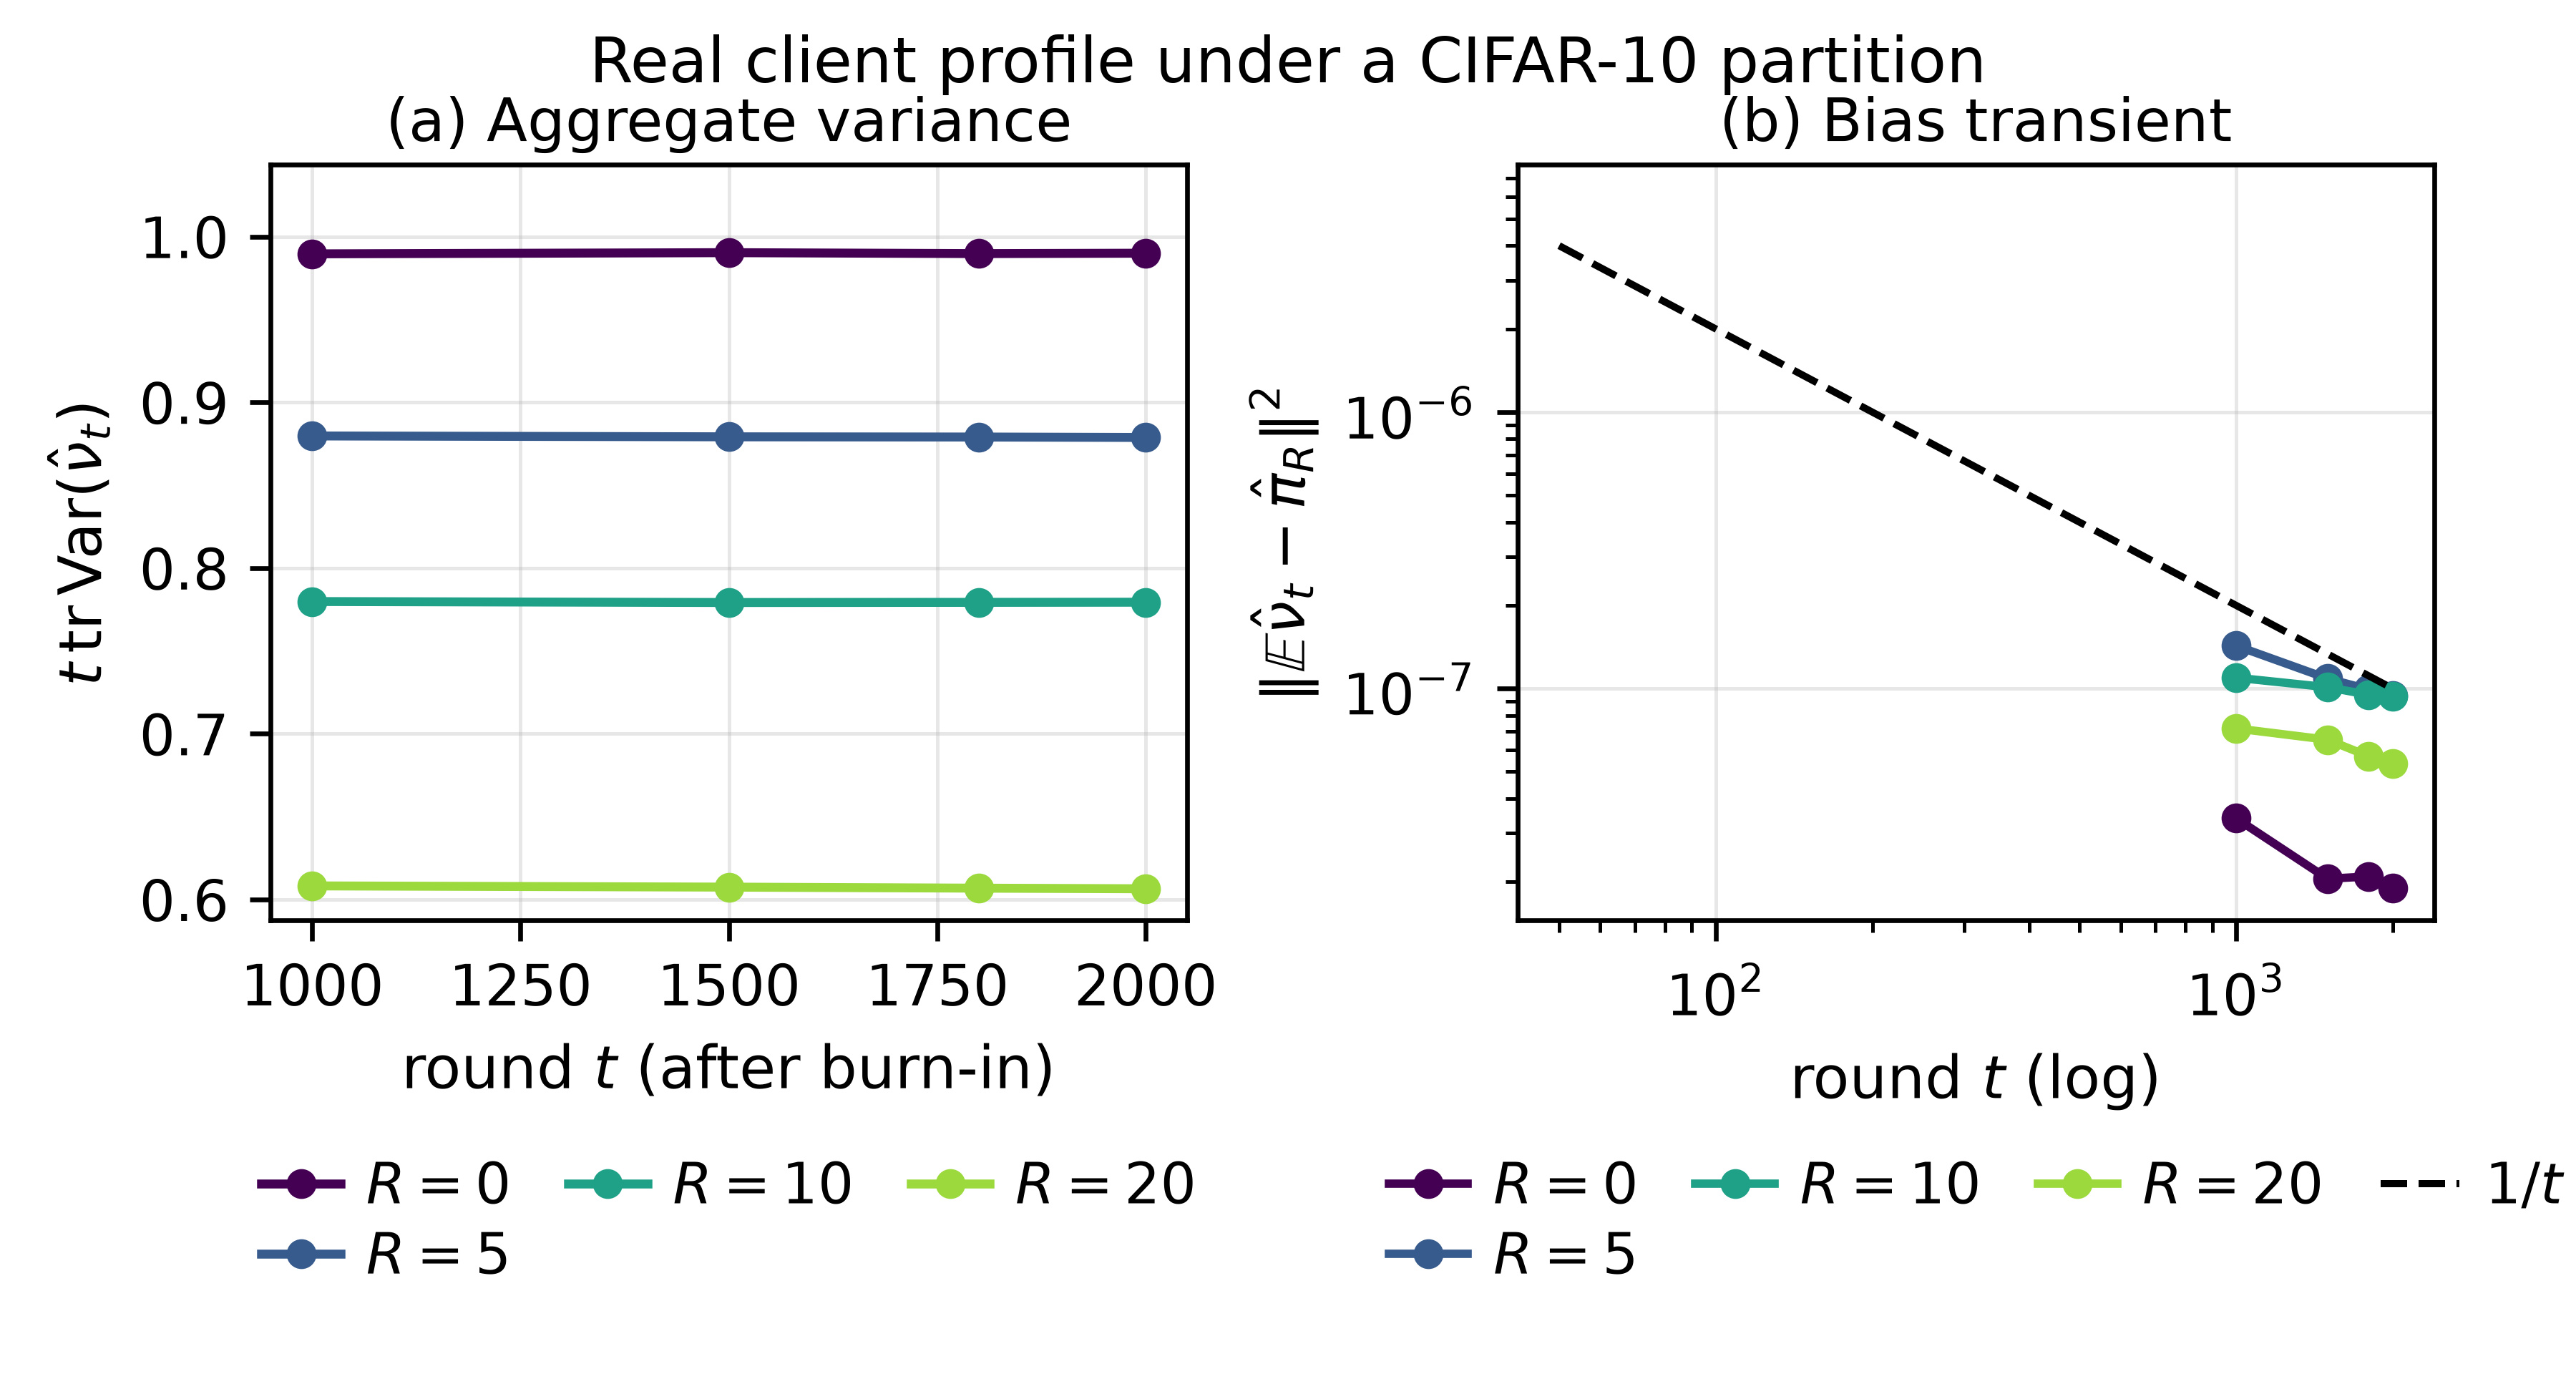
\includegraphics[width=\textwidth]{fig8.jpg}
\caption{Real client profile. (a) $t\,\mathrm{tr\,Var}(\hat\nu_t)$ under
the CIFAR-10 client profile at $t\in\{1000,1500,1800,2000\}$; (b) squared
bias transient with a $1/t$ reference slope.}
\label{fig:8}
\end{figure}

\textbf{E4a --- the $R=1$ aggregate criterion.} Theorem~3 gives a
closed-form inequality for whether the aggregate sampling variance
$\sum_i\sigma_i^2(R)$ increases from $R=0$ to $R=1$. On 36 random
propensity vectors the inequality agrees with an exact $N$-state Poisson
solve to $5.6\times10^{-16}$. The skewed profile of Proposition~1
satisfies the increase condition, with $\sum_i\sigma_i^2$ rising from
$0.0780$ to $0.3780$; the $N=100$ long-tailed profile of
Fig.~\ref{fig:3} instead falls from $0.7891$ to $0.6737$. Fractions of
Dirichlet$(\alpha_{\mathrm{Dir}})$ profiles satisfying the condition are reported in
Section~6.3.

\textbf{E4 --- uncertainty quantification.} With $10^{5}$
trajectories and $B_{\mathrm{boot}}=2000$ bootstrap resamples, at
$(N,R,\eta)=(20,16,0.04)$ the steady-state error is $0.01553$ (95\% CI
$[0.01547,0.01559]$) against the closed form $0.01559$; the measured ratio
to $R=0$ is $0.16810$ (analytic $0.168944$). Table~\ref{table:V} lists all
seven values. Fig.~\ref{fig:2} and Table~\ref{table:V} use independent
observation sets $\{b_k\}$ (seed $20261116$ with $4000$ trajectories and
seed $20261120$, respectively), hence different $C_0(f)$; by Proposition~3
their absolute errors differ by the constant scale
$C_0^{\mathrm{E4}}/C_0^{\mathrm{Fig.2}}\approx1.335$, while their ratios to $R=0$
agree; this experiment fixes $C_0(f)=4.5205$.
For Fig.~\ref{fig:3}, the aggregate variance at $R=0$ is
$0.79252$ (CI $[0.79012,0.79492]$) against $0.79354$, falling to $0.40014$
at $R=20$; every analytic reference value lies inside its interval.

\begin{table}[!t]
\small
\centering
\begin{tabular}{@{}cccc@{}}
\toprule
$R$ & measured & 95\% CI & Prop.~4 closed form \\
\midrule
0 & 0.09237 & [0.09198,0.09277] & 0.09226 \\
1 & 0.08333 & [0.08298,0.08370] & 0.08338 \\
2 & 0.07539 & [0.07507,0.07571] & 0.07526 \\
4 & 0.06125 & [0.06100,0.06153] & 0.06102 \\
8 & 0.03930 & [0.03913,0.03947] & 0.03914 \\
12 & 0.02423 & [0.02414,0.02433] & 0.02433 \\
16 & 0.01553 & [0.01547,0.01559] & 0.01559 \\
\bottomrule
\end{tabular}
\caption{Bootstrap validation of the Proposition 4 closed form at $10^5$ trajectories ($B_{\mathrm{boot}}=2000$): steady-state quadratic error of Fig.~\ref{fig:2}(b) with 95\% confidence intervals.}
\label{table:V}
\end{table}

\textbf{E5 --- real client profile.} A Dirichlet partition of CIFAR-10
training labels over $N=100$ clients supplies $p_i\propto n_i$ (no image
tensor is loaded and no model is trained). Fig.~\ref{fig:8}(a) reports
$t\,\mathrm{tr\,Var}(\hat\nu_t)$ at four checkpoints
($t\in\{1000,1500,1800,2000\}$) and (b) the squared bias
transient, which settles at the resolution of an independent estimate
$\hat\pi_R$ of the stationary participation vector; the $1/t$ line is a
reference slope.

All figures and tables are regenerated from the versioned release of
Section~1 by \texttt{make figures}. E5 uses $2\times10^{4}$
trajectories on the fixed seed recorded in \texttt{configs/default.yaml}.
\label{sec:experiments}

\section{Conclusion}
Minimum separation induces an $R$-th order participation chain. For
uniform availability we obtained $\sigma_i^{2}(R)$ and
$\tau_{\mathrm{int}}(R)$ in closed form, together with the steady-state error
of a constant-step-size linear estimator; both time scales are governed by
the degree-$R$ polynomial root $\lambda_\star(R,N)$ and move in opposite
directions with $R$: $\tau_{\mathrm{mix}}$ grows (Theorem~1, sharpened by
Theorems~4, 5 and~7) while $\tau_{\mathrm{int}}$ falls. Substituting
$\tau_{\mathrm{mix}}$ into the finite-time bound of \citep{ref1} yields an
explicit burn-in and step-size rule (Theorem~6). For general $p$ the
stationary window law (Proposition~5) and the $R=1$ variance (Theorem~3) are
explicit, and the aggregate variance reduces to a Poisson-solve tail.
Proposition~4 gives the covariance generating function and Corollary~4 the
idle-round variance. Finite-chain checks use exact state-space iteration.

\subsection{Scope and Limitations}
\begin{itemize}
\item \emph{Uniform availability and non-uniform profiles.} The
sampling-variance closed form, the spectral reduction, the prefactor bound,
and the multi-client and idle-round extensions assume $p_i\equiv1/N$. For
general $p$ the normalization of $P_R$ depends on the whole ordered window,
so the mixing time depends on the spectrum of $p$ and cannot be a function of
$(N,R)$ alone; finite-time bounds derived from the prefactor bound do not
apply. The stationary window law is closed form for any $(N,R,p)$, but the
aggregate-variance identity leaves the covariance tail to a Poisson solve;
the $R=0\to1$ criterion is a closed-form inequality.

\item \emph{Participation model and downstream optimizer.} Multiple clients
per round are covered only by the single-round marginal recursion; the mixing
time of that window chain is not covered, and non-fixed overlapping $K$-sets
admit a finite-dimensional transfer matrix but no scalar closed form.
All results hold on $R\le N-2$.

\item \emph{Mixing time beyond the main regime.} On $R\lesssim\sqrt{N/2}$
the mixing time is $R+O(1)$. Over the full aperiodic range, finiteness of
$C(q)$ follows from the filtration and the modulus bound of Appendix~C; a
prefactor independent of $(N,R)$, equivalently
$\tau_{\mathrm{mix}}=R+O(L)$ with an absolute constant, is open, and the
chi-square version is false in the tail regime.
\end{itemize}

\acks{This work received no external funding. The author declares no competing interests.}

\appendix
\section{\texorpdfstring{A Doeblin-Type Upper Bound on $\tau_{\mathrm{mix}}$}{A Doeblin-Type Upper Bound on tau mix}}
\textbf{Proposition A.1.} Let $N\geq2R+1$ and $p_i>0$ for all $i$. Then $P_R^{2R}(w,w')>0$ for all $w,w'\in\mathcal{S}_R$, whereas $P_R^{2R-1}$ has at least one zero entry; hence the least $s$ with $P_R^{s}(w,w')>0$ for all $w,w'\in\mathcal{S}_R$ is $s_0=2R$. Define the Doeblin coefficient
\begin{equation}\label{eq:e47}
\beta=\min_{w,w'\in\mathcal{S}_R}\dfrac{P_R^{2R}(w,w')}{\zeta_R(w')},
\end{equation}
so that $P_R^{2R}(w,\cdot)\geq\beta\,\zeta_R(\cdot)$ for all $w$.
Then $\beta\geq p_{\min}^{2R}$ and
\begin{equation}\label{eq:e48}
\tau_{\mathrm{mix}}(R)\leq2R\left\lceil\dfrac{\ln4}{\beta}\right\rceil,\quad \beta\geq\dfrac{(N)_R}{(N-R)^{2R}}\ \ \text{when } p_i\equiv1/N.
\end{equation}
\textbf{Proof.} Fix $w=(w_1,\dots,w_R)$ and $w'=(y_1,\dots,y_R)$. Choose the last $R$ injected clients as $x_{R+j}=y_{R-j+1}$ for $j=1,\dots,R$, so that the window at step $2R$ equals $w'$. Let $\mathcal{C}=[N]\setminus\{y_1,\dots,y_R\}$, with $|\mathcal{C}|=N-R\geq R+1$, and draw the first $R$ injections from $\mathcal{C}$. At step $j\leq R$ the forbidden set contains at most $R$ elements, so at least $|\mathcal{C}|-R\geq1$ admissible choices remain in $\mathcal{C}$; for $j>R$ the injected clients lie outside $\mathcal{C}$ and are distinct, hence no conflict arises. Every step has positive probability, so $P_R^{2R}(w,w')>0$. For $s=2R-1$ the final window $w'=(y_1,\dots,y_R)$ forces $y_R$ to be injected at step $R$, since the last $R$ injections must be $x_{R}=y_R,\dots,x_{2R-1}=y_1$. Immediately before step $R$ the window is $(x_{R-1},\dots,x_1,w_1)$, so $w_1$ is still forbidden and admissibility requires $y_R\neq w_1$. Taking $w=(1,\dots,R)$ and $w'=(2,\dots,R,1)$ gives $y_R=1=w_1$; hence no admissible injection sequence exists and $P_R^{2R-1}(w,w')=0$, so $s_0=2R$.

The minorization \citep{ref24} gives, by iterating $P_R^{2R}=\beta\zeta_R+(1-\beta)Q_{\mathrm{res}}$ with $Q_{\mathrm{res}}$ stochastic, $\max_w\|P_R^{2Rn}(w,\cdot)-\zeta_R\|_{\mathrm{TV}}\leq(1-\beta)^{n}\leq e^{-\beta n}$; choosing $n=\lceil\ln4/\beta\rceil$ yields the bound. Every admissible $2R$-step path has probability at least $p_{\min}^{2R}$ and $\zeta_R(w')\leq1$, which gives $\beta\geq p_{\min}^{2R}$. Under uniform availability, every such path has probability $(N-R)^{-2R}$ and $\zeta_R(w')=1/(N)_R$, so $\beta\geq(N)_R/(N-R)^{2R}$.

\section{An Explicit Tail-Covariance Bound}
For general $p$ and $R\leq N-2$, minimum separation gives $\mathrm{Cov}_k=-\pi_{R,i}^{2}$ for $1\leq k\leq R$, hence
\begin{equation}\label{eq:e49}
\sigma_i^{2}(R)=\pi_{R,i}(1-\pi_{R,i})-2R\pi_{R,i}^{2}+2\sum_{k>R}\mathrm{Cov}_k.
\end{equation}
The leading two terms are exact and identify the negative-lag contribution $-2R\pi_{R,i}^{2}$. When $N\geq2R+1$, Proposition A.1 gives, with the same Doeblin coefficient $\beta$, $\sup_w\|P_R^{k}(w,\cdot)-\zeta_R\|_{\mathrm{TV}}\leq(1-\beta)^{\lfloor k/(2R)\rfloor}$. Standard covariance decay for bounded functions yields $|\mathrm{Cov}_k|\leq2\pi_{R,i}(1-\pi_{R,i})(1-\beta)^{\lfloor k/(2R)\rfloor}$. Since $\sum_{k>R}(1-\beta)^{\lfloor k/(2R)\rfloor}\leq2R/\beta$, summing over $k>R$ gives
\begin{equation}\label{eq:e50}
\Big|\sum_{k>R}\mathrm{Cov}_k\Big| \leq\dfrac{4R\,\pi_{R,i}(1-\pi_{R,i})}{\beta}\quad \leq\dfrac{4R\,\pi_{R,i}(1-\pi_{R,i})}{p_{\min}^{2R}}.
\end{equation}
The prefactor $4R/\beta$ combines $2\pi_{R,i}(1-\pi_{R,i})$ with the
block sum $2R/\beta$. Under uniform availability the factor
$p_{\min}^{-2R}$ grows exponentially in $R$.

\section{Supplementary Material}
\label{app:supp}
\setcounter{subsection}{1}
\renewcommand{\thesubsection}{S.\arabic{subsection}}

This appendix supplies the derivations and numerical
certificates referred to above, for uniform availability $p_i\equiv1/N$ and
$1\le R\le N-2$ ($R=N-1$ is periodic and excluded). Write $m=N-R$,
\begin{equation}\label{eq:SR-p}
p_R(\lambda)=m\lambda^{R}+\lambda^{R-1}+\cdots+1,\qquad
\lambda_\star=\max_i|z_i|,\qquad L(R,N)=\frac{\ln4}{|\ln\lambda_\star|},
\end{equation}
with $z_1,\dots,z_R$ the roots of $p_R$ and $\alpha_0=m^R/(N)_R$; equation
numbering continues from the main text.

\textbf{Status of the material.} Sections~S.2--S.4 are proofs
(strong lumpability; the spectral filtration with its semisimplicity
argument; the Gelfand bound). Section~S.5 proves Theorem~7 with exact
rational certificates, Section~S.6 records the complex-valued TV duality,
Section~S.7 contains certificates and one open conjecture
(Conjecture~\ref{conj:G}), and Section~S.8 is a symbol table.

% ---------------------------------------------------------------------
\subsection{Strong lumpability and basic spectral facts}
\label{sec:S2}
% ---------------------------------------------------------------------

Let $\mathcal S_R$ be the set of ordered $R$-tuples of distinct labels in
$[N]$. The transition matrix of the window chain is
$P_R(w,(x,w_1,\dots,w_{R-1}))=1/m$ for $x\in \mathcal{C}(w)=[N]\setminus\{w_1,\dots,w_R\}$
and zero otherwise; its stationary law $\zeta_R$ is uniform on $\mathcal S_R$.
Let $a_0=(1,\dots,R)$ be the deterministic initial window.

\begin{slemma}[Strong lumpability and TV identity]\label{lem:A}
Under uniform availability, $P_R$ commutes with the action of the symmetric
group $\mathfrak{S}_{m}$ permuting the labels outside $a_0$. Partition $\mathcal S_R$
according to the identity of the initial label $a_i$ ($i\in[R]$) carried by
each coordinate, with $0$ denoting a fresh label; there are
$D_R=\sum_{k=0}^{R}\binom{R}{k}(R)_k$ classes, a number depending only on
$R$. For every $t\ge0$,
\begin{equation}\label{eq:S2-tv}
d_{\mathrm{TV}}(P_R^{t},\mathbf 1\zeta_R^{\top})
=\max_{w\in\mathcal S_R}\|\delta_wP_R^{t}-\zeta_R\|_{\mathrm{TV}}
=\|\delta_{a_0}q^{t}-\pi\|_{\mathrm{TV}},
\end{equation}
where $q$ is the lumped transition matrix and $\pi$ its stationary law.
\end{slemma}

\begin{proof}
For $\sigma\in \mathfrak{S}_m$ acting on the labels outside $a_0$, $P_R(w,w')=P_R(\sigma w,\sigma w')$,
because admissibility and the uniform draw from $\mathcal{C}(w)$ depend only on the set
of labels in the window, not on their particular identities. Hence $P_R$ commutes
with the group action. The initial state $a_0$ is fixed by $\mathfrak{S}_m$, so
$\delta_{a_0}P_R^{t}$ is constant on each orbit, i.e.\ on each class; the
uniform law $\zeta_R$ is constant on each class as well. The total-variation
distance between two class-constant measures equals the total-variation
distance of their class masses, which is the right-hand side. The maximum over
$w$ is attained at $a_0$ because all classes with the same cardinality have
the same $\zeta_R$-mass and $\delta_wP_R^{t}$ is concentrated on a single
class at $t=0$.
\end{proof}

A class $c$ with $k_c$ retained initial labels has stationary weight
$\pi(c)=(m)_{R-k_c}/(N)_R$ and is reachable only if $R-k_c\le m$, i.e.\
$k_c\ge 2R-N$. Retaining unreachable classes produces spurious Jordan blocks;
with the reachable state space one has $\pi q=\pi$ to $10^{-16}$ on all
certified chains. The lumped transition is
\begin{equation}\label{eq:S2-q}
q\big(c\to(0,c_1,\dots,c_{R-1})\big)=\frac{m-R+k_c}{m},\qquad
q\big(c\to(a_j,c_1,\dots,c_{R-1})\big)=\frac{1}{m},
\end{equation}
the latter for each initial label $a_j$ not retained in $c$. Recording
\emph{which} $a_i$ is retained is necessary. A lump that records only
``initial vs.\ fresh'' merges distinct classes and underestimates TV (it
gives $5$ instead of $7$ for $\tau_{\mathrm{mix}}$ at $(N,R)=(10,4)$).

\begin{slemma}[No repeated roots]\label{lem:squarefree}
$p_R$ has $R$ distinct roots and $\lambda_\star<1$ for $1\le R\le N-2$.
\end{slemma}

\begin{proof}
Multiply by $\lambda-1$:
$\Psi(\lambda)=(\lambda-1)p_R(\lambda)=m\lambda^{R+1}-(m-1)\lambda^{R}-1$.
Its derivative vanishes at $\lambda=0$ and at the single nonzero critical
point $\lambda_0=R(m-1)/((R+1)m)$, where $\Psi(\lambda_0)<-1<0$; hence $\Psi$ and
$\Psi'$ share no root, and $\Psi(1)=0$, $\Psi'(1)=N+1\ne0$ give that $1$ is a simple
root of $\Psi$. Therefore $p_R$ is squarefree. If $|\lambda|\ge1$ were a root of
$p_R$, then
$m|\lambda|^{R+1}=|(m-1)\lambda^{R}+1|\le(m-1)|\lambda|^{R}+1\le m|\lambda|^{R}$,
forcing $|\lambda|=1$ and $\lambda^{R}=1$, hence $\lambda=1$; but
$p_R(1)=N\ne0$.
\end{proof}

\textbf{Certificate.} For $(N,R)=(6,2),(8,3)$, direct iteration of
the full $(N)_R$-dimensional $P_R$ and of $q$ agree in
\eqref{eq:S2-tv} to $4.4\times10^{-16}$ for all $t\le R+6$
(\texttt{check\_spectral.py}).

% ---------------------------------------------------------------------
\subsection{\texorpdfstring{Spectral filtration and the $j\ge2$ blocks}{Spectral filtration and the j at least 2 blocks}}
\label{sec:S3}
% ---------------------------------------------------------------------

Let $\mathcal{F}$ be the algebra of functions on $\mathcal S_R$ generated by
the coordinate indicators $u_{k,a}(w)=\mathbf{1}\{w_k=a\}$, $1\le k\le R$,
$a\in[N]$. Let $V_{\le j}\subset\mathcal{F}$ be spanned by products of at
most $j$ such indicators. Because the draw is uniform on the complement,
\begin{equation}\label{eq:S3-cond}
\mathbb E\big[\,\mathbf{1}\{X_1=a\}\mid Y_0=w\,\big]
=\frac{1-\sum_{l=1}^{R}\mathbf{1}\{w_l=a\}}{m}.
\end{equation}
\begin{sprop}[Filtration]\label{prop:filtration}
For each $j\ge1$, $P_RV_{\le j}\subseteq V_{\le j}$, so $P_R$ is block upper
triangular with respect to $(V_{\le j})_j$. On the quotient
$V_{\le j}/V_{\le j-1}$ its spectrum is contained in
$\{z_{i_1}\cdots z_{i_j}:1\le i_1,\dots,i_j\le R\}$; consequently the
$j$-th block has spectral radius at most $\lambda_\star^{j}$. In particular the
$j\ge2$ blocks have modulus at most $\lambda_\star^{2}$, and the companion
($j=1$) block alone carries the spectral radius $\mathrm{spr}(q-\Pi)=\lambda_\star$.
\end{sprop}

\begin{proof}
One step maps the window to $Y_1=(X_1,w_1,\dots,w_{R-1})$, so coordinate
$k$ becomes $k+1$; the last coordinate $w_R$ leaves the window. Let
$\Phi=\prod_{s=1}^{j}u_{k_s,a_s}$ with distinct coordinates. If no
$k_s=1$ is needed, $P_R\Phi$ is the same product with each index shifted,
up to terms in which a repeated coordinate produces a lower-degree product
(when two shifted indices coincide, $\mathbf{1}\{w_k=a\}\mathbf{1}\{w_k=b\}=\mathbf{1}\{a=b\}\mathbf{1}\{w_k=a\}$).
If the new coordinate $1$ is one of the factors, \eqref{eq:S3-cond}
replaces $\mathbf{1}\{X_1=a\}$ by $m^{-1}(1-\sum_l\mathbf{1}\{w_l=a\})$; the constant part
drops the degree by one and the sum produces $j$-fold products again. Hence
$P_R\Phi\in V_{\le j}$.

On the quotient, only the degree-preserving part survives. Each of the $j$
factors evolves independently under the coordinate shift $k\mapsto k-1$
with the rank-one correction $-\frac1m\mathbf 1 \mathbf{e}_1^{\top}$; this is the
companion matrix $B^{\top}$ of Theorem~4, whose characteristic
polynomial is $p_R(\lambda)/m$. The induced operator on the quotient is
therefore a restriction of $(B^{\top})^{\otimes j}$ to the subspace spanned
by products at distinct coordinates, composed with the permutation
representation of $\mathfrak{S}_j$ that relabels the factors. Any eigenvalue of a
restriction of a tensor power is a product $z_{i_1}\cdots z_{i_j}$ up to the
eigenvalues of that permutation representation, which have modulus one;
hence every eigenvalue of the quotient has modulus at most
$(\max_i|z_i|)^{j}=\lambda_\star^{j}$. Since $\lambda_\star<1$ by Lemma~\ref{lem:squarefree},
$\lambda_\star^{j}\le\lambda_\star^{2}<\lambda_\star$ for $j\ge2$, and the $j=1$ block, whose eigenvalues
are exactly $z_1,\dots,z_R$, carries the spectral radius.
\end{proof}

\begin{scor}[Finiteness of $C(q)$]\label{cor:Cfinite}
Let $v_0=\delta_{a_0}q^{R}-\pi$ and
$C(q)=\sup_{s\ge1}d(R+s)/\lambda_\star^{s}$ as in equation~\eqref{eq:e28}.
Then $C(q)<\infty$ and is independent of $(N)_R$.
\end{scor}

\begin{proof}
By Proposition~\ref{prop:filtration} every eigenvalue of $q-\Pi$ has modulus
$\le\lambda_\star$, and those of modulus exactly $\lambda_\star$ lie in the companion
($j=1$) layer. That layer carries $R^2$ eigenvalues (Table~\ref{tab:S3}):
the $R$ distinct roots of $p_R$, each with multiplicity. Lemma~\ref{lem:squarefree}
therefore diagonalises the $R\times R$ companion matrix $B^\top$ but does not
by itself exclude Jordan chains of $q$ at modulus $\lambda_\star$. To rule them out,
let $\mathcal{G}=\mathfrak{S}_{m}$ act on the labels outside the initial window $a_0$, as in Lemma~\ref{lem:A}. Both $P_R$ and
the lumping projection are $\mathcal{G}$-equivariant, so the filtration $(V_{\le j})_j$
of Proposition~\ref{prop:filtration} consists of $\mathcal{G}$-submodules. Over a field
of characteristic zero and for finite $\mathcal{G}$, Maschke's theorem makes each
$V_{\le j}$ completely reducible: choose $\mathcal{G}$-invariant complements $W_j$ with
$V_{\le j}=V_{\le j-1}\oplus W_j$ and the corresponding $\mathcal{G}$-equivariant
projections. The lumped states are precisely the $\mathcal{G}$-orbits on $\mathcal{S}_R$,
so functions on the class space are the $\mathcal{G}$-invariant functions on
$\mathcal{S}_R$, and the Maschke splitting above restricts to this invariant
part. Since $P_R$ commutes with $\mathcal{G}$ it preserves every $W_j$, and $q$
is similar to $\bigoplus_j M_j$ with $M_j=P_R|_{W_j}$. On $W_1$ the induced
operator is $B^\top\otimes\Xi_1$, with $\Xi_1$ a permutation representation
of $\mathcal{G}$; decomposing $\Xi_1$ into irreducibles $\rho$ of dimension
$d_\rho$ and applying Schur's lemma gives
$M_1\cong\bigoplus_\rho\bigl(B^\top\otimes I_{d_\rho}\bigr)$ on the
$\mathcal{G}$-isotypic components. As $p_R$ is squarefree, $B^\top$ has $R$ distinct
eigenvalues and is diagonalisable; hence $M_1$ is semisimple and every
eigenvalue of modulus $\lambda_\star$ has trivial Jordan blocks. The $j\ge2$ layers
have modulus $\le\lambda_\star^2<\lambda_\star$, so any Jordan blocks there are suppressed by
$\lambda_\star^{-m}$. Consequently
$\sup_{s\ge0}\|(q-\Pi)^{s}/\lambda_\star^{s}\|_{1\to1}<\infty$, and
$d(R+s)=\tfrac12\|v_0(q-\Pi)^{s}\|_{1}$ with $\|v_0\|_1\le2$ gives the claim.
The bound depends only on the $D_R$-dimensional matrix $q$.
\end{proof}

\textbf{Certificate (Table~\ref{tab:S3}).} For each chain, the
number of non-trivial eigenvalues of $q$ with modulus strictly above
$\lambda_\star^2$ equals $R^2$ (the companion block with its multiplicity), and the
largest modulus among all remaining eigenvalues equals $\lambda_\star^2$ exactly.
This is computed by dense eigendecomposition of $q$ in
\texttt{check\_spectral.py}.

\begin{table}[htbp]
\centering
\begin{tabular}{cclcc}
\toprule
$(N,R)$ & $D_R$ & $\lambda_\star$ & companion ($R^2$) & rest$/\lambda_\star^2$ \\
\midrule
(6,2) & 7 & 0.500000 & 4 & 1.000000 \\
(7,2) & 7 & 0.447214 & 4 & 1.000000 \\
(8,2) & 7 & 0.408248 & 4 & 1.000000 \\
(8,3) & 34 & 0.613390 & 9 & 1.000000 \\
(9,3) & 34 & 0.577350 & 9 & 1.000000 \\
(12,3) & 34 & 0.503926 & 9 & 1.000000 \\
(8,4) & 209 & 0.758414 & 16 & 1.000000 \\
(10,4) & 209 & 0.687482 & 16 & 1.000000 \\
(12,4) & 209 & 0.639925 & 16 & 1.000000 \\
(10,5) & 1546 & 0.788142 & 25 & 1.000000 \\
\bottomrule
\end{tabular}
\caption{Spectral filtration certificate. $D_R$ is the lumped state-space
size; ``companion'' counts eigenvalues with $|\lambda|>\lambda_\star^2$; ``rest'' is
the largest modulus of the remaining non-trivial eigenvalues.}
\label{tab:S3}

\end{table}
% ---------------------------------------------------------------------
\subsection{\texorpdfstring{Gelfand bound and the constant $C_{\mathrm{gel}}$}{Gelfand bound and the constant C gel}}
\label{sec:S4}
% ---------------------------------------------------------------------

Let $\Pi=\mathbf 1\pi^{\top}$, $\bar q=q-\Pi$. Since
$\Pi q=q\Pi=\Pi$, one has $\bar q^{s}=q^{s}-\Pi$ for $s\ge1$; since
$v_0\Pi=0$,
\begin{equation}\label{eq:S4-d}
d(R+s)=\tfrac12\|v_0\bar q^{s}\|_{1}
\le\tfrac12\|v_0\|_{1}\,\|\bar q^{s}\|_{1\to1}
\le\|\bar q^{s}\|_{1\to1},
\end{equation}
using $\|v_0\|_1\le2$ (difference of two probability measures).

\begin{sprop}[Gelfand bound]\label{prop:gelfand}
For every $\epsilon_{\mathrm{gel}}\in(0,1-\lambda_\star)$ there exists $C_{\mathrm{gel}}<\infty$,
depending only on the $D_R$-dimensional matrix $q$ and on $\epsilon_{\mathrm{gel}}$,
with
\begin{equation}\label{eq:S4-gelfand}
\|\bar q^{s}\|_{1\to1}\le C_{\mathrm{gel}}(\lambda_\star+\epsilon_{\mathrm{gel}})^{s},
\qquad s\ge0.
\end{equation}
With $\epsilon_{\mathrm{gel}}=\sqrt{\lambda_\star}-\lambda_\star$ one obtains
$\lambda_\star+\epsilon_{\mathrm{gel}}=\sqrt{\lambda_\star}$ exactly, hence
\begin{equation}\label{eq:S4-tau}
\tau_{\mathrm{mix}}(R)\le R+2L(R,N)+\frac{2\ln C_{\mathrm{gel}}}{|\ln\lambda_\star|}.
\end{equation}
\end{sprop}

\begin{proof}
By Proposition~\ref{prop:filtration}, $\mathrm{spr}(\bar q)=\lambda_\star$. The Gelfand
formula $\mathrm{spr}(\bar q)=\lim_{s\to\infty}\|\bar q^{s}\|^{1/s}$ holds for any
operator norm on the finite-dimensional space $\mathbb R^{D_R}$, so for any
$\epsilon_{\mathrm{gel}}>0$ the sequence
$\|\bar q^{s}\|_{1\to1}/(\lambda_\star+\epsilon_{\mathrm{gel}})^{s}$ is bounded; its supremum is
the finite $C_{\mathrm{gel}}$. Requiring $C_{\mathrm{gel}}(\lambda_\star+\epsilon_{\mathrm{gel}})^{s}
\le1/4$ gives
$s\ge\ln(4C_{\mathrm{gel}})/|\ln(\lambda_\star+\epsilon_{\mathrm{gel}})|$. With
$\lambda_\star+\epsilon_{\mathrm{gel}}=\sqrt{\lambda_\star}$ we have
$|\ln(\lambda_\star+\epsilon_{\mathrm{gel}})|=\tfrac12|\ln\lambda_\star|$, whence \eqref{eq:S4-tau}.
\end{proof}

\begin{srem}[On the choice of $\epsilon_{\mathrm{gel}}$]\label{rem:S4-eps}\upshape
Taking $\epsilon_{\mathrm{gel}}=(1-\lambda_\star)/2$ would give \eqref{eq:S4-tau} only if
$|\ln((1+\lambda_\star)/2)|\ge\tfrac12|\ln\lambda_\star|$, but the inequality is reversed.
By AM--GM,
$(1+\lambda_\star)/2\ge\sqrt{\lambda_\star}$, so
$|\ln((1+\lambda_\star)/2)|\le\tfrac12|\ln\lambda_\star|$ for $0<\lambda_\star<1$. Numerically at
$\lambda_\star=0.5$ the two sides are $0.2877$ and $0.3466$. The choice
$\epsilon_{\mathrm{gel}}=\sqrt{\lambda_\star}-\lambda_\star$ is admissible because
$0<\sqrt{\lambda_\star}-\lambda_\star<1-\lambda_\star$ for $0<\lambda_\star<1$, and it makes the equality exact.
\end{srem}

\textbf{Non-uniformity of $C_{\mathrm{gel}}$.}
Table~\ref{tab:S4} reports the lower bound
$\sup_{1\le s\le120}\|\bar q^{s}\|_{1\to1}/(\sqrt{\lambda_\star})^{s}$, which grows
with $N$ at fixed $R$. A bound on $C(q)$
independent of $(N,R)$ is Conjecture~\ref{conj:G} below.

\begin{table}[htbp]
\centering
\begin{tabular}{ccccc}
\toprule
$(N,R)$ & $D_R$ & $\lambda_\star$ & $\sqrt{\lambda_\star}$ & $C_{\mathrm{gel}}\ \ge$ \\
\midrule
(6,2) & 7 & 0.50000 & 0.70711 & 2.451 \\
(12,2) & 7 & 0.31623 & 0.56234 & 3.287 \\
(20,2) & 7 & 0.23570 & 0.48549 & 3.924 \\
(40,2) & 7 & 0.16222 & 0.40277 & 4.845 \\
(80,2) & 7 & 0.11323 & 0.33649 & 5.870 \\
(9,3) & 34 & 0.57735 & 0.75984 & 3.217 \\
(20,3) & 34 & 0.40618 & 0.63732 & 4.716 \\
(40,3) & 34 & 0.31153 & 0.55815 & 6.272 \\
(12,4) & 209 & 0.63992 & 0.79995 & 3.739 \\
(30,4) & 209 & 0.47287 & 0.68766 & 5.986 \\
\bottomrule
\end{tabular}
\caption{Lower bounds on $C_{\mathrm{gel}}$ for $\epsilon_{\mathrm{gel}}=\sqrt{\lambda_\star}-\lambda_\star$.
Computed by exact dense iteration of the lumped chain in
\texttt{check\_gelfand.py}.}
\label{tab:S4}

\end{table}

\textbf{Three constants.} $C(q)=\sup_{s\ge1}d(R+s)/\lambda_\star^{s}$ is the
tight prefactor of Theorem~5; $C_{\mathrm{spec}}(q)$ is the
sum-of-projections quantity in equation~\eqref{eq:e45} and is a
feasible upper bound on $C(q)$ once the full block diagonalisation is
available; $C_{\mathrm{gel}}$ is the Gelfand constant above and has no uniform bound.

% ---------------------------------------------------------------------
\subsection{\texorpdfstring{One-step $\chi^2$ contraction (Theorem~7)}{One-step chi squared contraction (Theorem 7)}}
\label{sec:S5}
% ---------------------------------------------------------------------

After $R$ steps the law of the lumped chain is $\mu_R=\pi|_{\mathcal{A}}/\alpha_0$,
where $\mathcal{A}$ is the $R$-step reachable set with $\pi(\mathcal{A})=\alpha_0$. Write
$h_0=\alpha_0^{-1}\mathbf{1}\{\mathcal{A}\}$ and
$\chi^2_s=\|(q^{*})^{s}(h_0-1)\|_{L^2(\pi)}^{2}$, with $q^*$ the
$\pi$-adjoint of $q$.

\begin{sprop}[One-step Radon--Nikodym derivative]\label{prop:rho}
Let $k_y$ count the retained initial labels in $y$, $t_y=m-R+k_y$, and let
$\mathcal{B}$ be the set of states whose coordinate $r\ge2$ is either $0$ or an
initial label $\ge r$. Then
\begin{equation}\label{eq:S5-rho}
\rho(y):=\sum_{x\in\mathcal{A}}\frac{\pi(x)q(x,y)}{\pi(y)}
=\frac{t_y}{m}\,\mathbf{1}\{y\in\mathcal{B}\},\qquad \mathbb E_{\pi}[\rho]=\alpha_0,
\end{equation}
and, with $T_j:=\sum_{y\in\mathcal{B}}(m)_{R-k_y+j}$,
\begin{equation}\label{eq:S5-Sj}
T_j=(m)_{j-1}(m-j+1)^{R+1},\qquad
\mathbb E_{\pi}[\rho^{2}]=\frac{T_2+T_1}{m^{2}(N)_R}.
\end{equation}
Consequently
$\chi^2_0=\alpha_0^{-1}-1$ and
$\chi^2_1=A_c\alpha_0^{-1}-1$ with
$A_c=(1-1/m)^{R+1}+1/m<1$.
\end{sprop}

\begin{proof}
At step $R$ the defining condition of $\mathcal{A}$ cannot hold with a nonzero last
coordinate, so every $x\in\mathcal{A}$ has $x_R=0$. A predecessor of $y$ has the form
$x=(y_2,\dots,y_R,x_R)$, and $x\in\mathcal{A}$ forces $x_R=0$; hence at most one
predecessor contributes, which gives \eqref{eq:S5-rho} after cancelling
$\pi(x)/\pi(y)$ against the transition probability. Using
$t^{2}=(t)_2+t$ and collecting terms gives \eqref{eq:S5-Sj}. Both sides of
the identity $T_j=(m)_{j-1}(m-j+1)^{R+1}$ are polynomials in $m$ of degree
at most $R+j$; the two sides agree at $R+j+2$ distinct integer
values of $m$ by exact rational enumeration, hence the polynomial identity.
\end{proof}

Since $q^*$ is a $\pi$-stationary Markov operator, Jensen's inequality gives
$\|q^*f\|_{2,\pi}\le\|f\|_{2,\pi}$; with $q^*\mathbf 1=\mathbf 1$ and
$h_0-1\perp\mathbf 1$, $\chi^2_s$ is nonincreasing. Cauchy--Schwarz gives
$d(R+s)\le\tfrac12\sqrt{\chi^2_s}\le\tfrac12\sqrt{\chi^2_1}$ for all
$s\ge1$, hence $\chi^2_1\le1/4$ implies $\tau_{\mathrm{mix}}\le R+1$. Solving the exact
rational inequality gives the minimal admissible $m$ for each $R$;
asymptotically $m\gtrsim2R^{2}$, i.e.\ $R\lesssim\sqrt{N/2}$.

\textbf{Maximal coupling.} An independent bound avoids
$\chi^2$ entirely. At each step, given windows $w,w'$, draw a single label
from $\mathcal{C}(w)\cap\mathcal{C}(w')$ with probability $|\mathcal{C}(w)\cap\mathcal{C}(w')|/m$ and let the two
chains draw independently from their complements otherwise. Since
$|\mathcal{C}(w)\cap\mathcal{C}(w')|\ge N-2R$, the coincidence probability is at least
$1-R/m$ when $N\ge2R$. After $R$ consecutive coincidences the two windows
are identical, and with identical windows the same uniform draw keeps them
identical forever. Splitting time into disjoint blocks of length $R$, each
block succeeds with probability at least $(1-R/m)^{R}\ge1-R^{2}/m\ge3/4$
when $m\ge4R^{2}$, so one block suffices and $\tau_{\mathrm{mix}}\le2R$.
\texttt{check\_chi2.py} gives a numerical illustration of $\tau_{\mathrm{mix}}\le2R$ at $R=2,\dots,6$ with $m=4R^{2}$; the bound itself is the constructive coupling above.

\begin{srem}[Rank-based common random numbers]\label{rem:S5-rank}\upshape
Ordering each complement as $\ell_1<\dots<\ell_m$ and using the same uniform rank
for both chains does \emph{not} give coincidence probability
$|\mathcal{C}\cap\mathcal{C}'|/m$. Take $\mathcal{C}=\{1,2,3\}$, $\mathcal{C}'=\{2,3,4\}$: the intersection has
size $2$, but the rank pairs are $(1,2),(2,3),(3,4)$ and never coincide.
The bound above uses an explicit maximal coupling instead.
\end{srem}

\textbf{The case $R=2$.} Here $\lambda_\star=(N-2)^{-1/2}$ identically,
$\tau_\star:=\lambda_\star^{2}=1/m$, and the generating function
$F(z)=\sum_{s\ge0}\chi^2_s z^{s}=P_\chi(z)/Q_\chi(z)$ has four simple poles
$\{z_1^{2},z_2^{2},\tau_\star,\tau_\star^{2}\}$, all of modulus $\le\tau_\star$. Writing
$F(z)=\sum_k A_k/(1-\omega_k z)$ gives
$\chi^2_s\le(\sum_k|A_k|)\tau_\star^{s}$. Table~\ref{tab:S5-R2} lists
$\sum_k|A_k|$; its maximum over $N\ge6$ is $1.449219$ at $N=6$, and it
decreases to $1$ as $N\to\infty$. For the two smallest admissible chains the
constant is larger, so the bound
$\chi^2_s\le1.4492\,\lambda_\star^{2s}$ is stated for $N\ge6$ in Section~4.

\begin{table}[htbp]
\centering
\begin{tabular}{ccccccc}
\toprule
$N$ & 4 & 5 & 6 & 7 & 8 & 10 \\
\midrule
$\sum_k|A_k|$ & 2.241071 & 1.671156 & 1.449219 & 1.334821 & 1.265935 & 1.187697 \\
\bottomrule
\end{tabular}
\caption{$R=2$: sum of absolute residues of $P_\chi/Q_\chi$
(\texttt{check\_chi2.py}, \texttt{check\_gelfand.py}).}
\label{tab:S5-R2}

\end{table}
% ---------------------------------------------------------------------
\subsection{Complex-valued TV duality (Theorem~4)}
\label{sec:S6}
% ---------------------------------------------------------------------

The lower bound \eqref{eq:e19} uses a possibly complex
eigenfunction $\varphi$ of $P_R$ with eigenvalue $\lambda$,
$|\lambda|=\lambda_\star$, and $\zeta_R\varphi=0$. The dual norm is
\begin{equation}\label{eq:S6-dual}
\|\mu-\nu\|_{\mathrm{TV}}
=\tfrac12\sup_{\substack{|\psi|\le1\\ \psi\in\mathbb C}}
\big|\mathbb E_{\mu}\psi-\mathbb E_{\nu}\psi\big|,
\end{equation}
which follows from the real-valued duality together with
$|\mathbb E\psi|=\sup_{\omega}\mathbb E\operatorname{Re}(e^{\mathrm{j}\omega}\psi)$.
Applying \eqref{eq:S6-dual} with $\psi=\varphi/\|\varphi\|_\infty$ at a window
$w$ attaining $|\varphi(w)|=\|\varphi\|_\infty$ gives
$d_{\mathrm{TV}}(P_R^{t},\mathbf 1\zeta_R^{\top})
\ge|(P_R^{t}\varphi)(w)-\zeta_R\varphi|/(2\|\varphi\|_\infty)
=\lambda_\star^{t}/2$, hence $\tau_{\mathrm{mix}}\ge\max\{R,\lceil\ln2/|\ln\lambda_\star|\rceil\}$ after
combining with Theorem~1.

% ---------------------------------------------------------------------
\subsection{Tail-regime certificates and the open conjecture}
\label{sec:S7}
% ---------------------------------------------------------------------

\begin{sconj}[Uniform $\ell^1$ prefactor]\label{conj:G}
There is an absolute constant $C_{\mathrm{unif}}$ such that
$\|v_0q^{s}\|_{1}\le C_{\mathrm{unif}}\lambda_\star^{s}\|v_0\|_{1}$ for all $s\ge0$ and all
$1\le R\le N-2$. This is a \emph{sufficient} condition for
$\tau_{\mathrm{mix}}(R)=R+O(L(R,N))$ with an absolute constant on the whole aperiodic
range, because $\ln C_{\mathrm{unif}}$ is a constant multiple of $L(R,N)$.
\end{sconj}

The conjecture is open on the upper-bound side; the matching
lower bound $\tau_{\mathrm{mix}}\ge\max\{R,\lceil\ln2/|\ln\lambda_\star|\rceil\}$ is a theorem
on the whole aperiodic range (Sections~S.2, S.6).

\textbf{Failure of the chi-square analogue.} With
$\alpha_0=m^R/(N)_R$ and $\chi^2_1=A_c\alpha_0^{-1}-1$, the ratio
$\chi^2_1/\lambda_\star^{2}$ diverges in the tail regime. It equals
$3.79\times10^{3}$, $1.22\times10^{5}$, $5.46\times10^{6}$ and
$3.25\times10^{8}$ at $(N,R)=(10,8),(12,10),(14,12),(16,14)$, with
$\alpha_0=1.41\times10^{-4},4.28\times10^{-6},9.40\times10^{-8},
1.57\times10^{-9}$ and
$\chi^2_1=3.56\times10^{3},1.17\times10^{5},5.32\times10^{6},
3.19\times10^{8}$ respectively (exact rational closed form). No bound
$\chi^2_s\le K_{\mathrm{env}}\lambda_\star^{2s}$ with $K_{\mathrm{env}}$ independent
of $(N,R)$ exists: $\|v_0\|_1=2(1-\alpha_0)\le2$ keeps the $\ell^1$ quantity
bounded, whereas $\chi^2_0=\alpha_0^{-1}-1$ grows like $\alpha_0^{-1}$ and
Cauchy--Schwarz loses a factor $\sqrt{\alpha_0}$ there.
\begin{table}[htbp]
\centering
\begin{tabular}{ccc@{\qquad}ccc}
\toprule
$(N,R)$ & prefactor & & $(N,R)$ & prefactor & \\
\midrule
(6,2) & 0.4594 && (15,3) & 0.4513 \\
(7,2) & 0.4217 && (29,4) & 0.4625 \\
(8,3) & 0.5825 && (71,6) & 0.5294 \\
(8,4) & 0.8468 && (20,6) & 0.8747 \\
(10,5) & 0.9476 && (100,7) & 0.5749 \\
(10,8) & 1.4817 && (9,3) & 0.5555 \\
(12,10) & 1.3052 && (11,4) & 0.7297 \\
(14,12) & 1.1914 && (13,6) & 0.9938 \\
(30,4) & 0.4540 && (50,5) & 0.4682 \\
(200,6) & 0.3848 && & & \\
\bottomrule
\end{tabular}
\caption{Exact TV prefactor certificates (\texttt{check\_certificates.py}).}
\label{tab:S7-pref}

\end{table}

\textbf{Certificate inventories.} Table~\ref{tab:S7-inv}
collects three disjoint sets of exact certificates. Since $C(q)$ is
\emph{defined} by $C(q)=\sup_{s\ge1}d(R+s)/\lambda_\star^{s}$, \eqref{eq:e28} holds
by construction; Tables~3--4 report the measured magnitude of $C(q)$ and its
comparison with $L$, not a test of the inequality.
Table~\ref{tab:S7-pref} is an independent recomputation on $19$ chains
spanning the main, intermediate and tail regimes, including chains with
$R>N/2$; $\alpha_0$ reaches $9.40\times10^{-8}$ and the largest prefactor
is $1.4817$ at $(N,R)=(10,8)$. \texttt{check\_algebra.py} compares
$\chi^2_1=A_c/\alpha_0-1$ against exact forward iteration on $22$ pairs.

\begin{table}[htbp]
\centering
\begin{tabular}{@{}lcl@{}}
\toprule
Source & chains & reported quantity \\
\midrule
Tables~3--4 (main text) & $22$ & $C(q)\in[0.010,1.575]$ \\
Table~\ref{tab:S7-pref} & $19$ & $\sup_s d(R+s)/\lambda_\star^{s}\le1.4817$ \\
\texttt{check\_algebra.py} & $22$ & $\chi^2_1$ vs.\ iteration, $\le3.6\times10^{-15}$ \\
\bottomrule
\end{tabular}
\caption{Certificate inventories. All three sets are exact finite-chain
computations; none is used as a theorem.}
\label{tab:S7-inv}
\end{table}

\textbf{Unconditional bounds on the tail regime.} Four bounds are
available without the spectral-block identification of
Section~\ref{sec:S3}: (i) the Gelfand bound \eqref{eq:S4-tau} with
$C_{\mathrm{gel}}$ tabulated in Table~\ref{tab:S4}; (ii)
$d(R+s)\le\tfrac12\sqrt{\chi^2_1}$ from Proposition~\ref{prop:rho}; (iii)
$\chi^2_s\le1.4492\,\lambda_\star^{2s}$ for $R=2$, $N\ge6$
(Table~\ref{tab:S5-R2}); and (iv) maximal coupling. In general form,
splitting time into blocks of length $R$ gives
\begin{equation}\label{eq:S7-coupling}
\tau_{\mathrm{mix}}(R)\le R\Big(1+\frac{\ln4}{|\ln(1-\gamma_{\mathrm{cpl}})|}\Big),\qquad
\gamma_{\mathrm{cpl}}=(1-R/m)^{R},
\end{equation}
valid for every $N\ge2R$, using only $Y_t=(X_t,\dots,X_{t-R+1})$ and none of
the roots of $p_R$, diagonalisability, the filtration or $\chi^2$. For $m=O(R)$ it is loose by $e^{\Theta(R)}$; $m\ge4R^2$ gives
$\tau_{\mathrm{mix}}\le2R$.

% ---------------------------------------------------------------------
\subsection{Symbols}
\label{sec:S8}
% ---------------------------------------------------------------------

\setlength{\LTleft}{0pt}
\setlength{\LTright}{\fill}
\begin{longtable}{@{}lp{3.30in}@{}}
$N$, $R$, $[N]$, $(N)_R$ & clients; minimum separation; label set; falling factorial \\
$s$, $m=N-R$, $s_0=2R$ & steps beyond the first $R$ rounds; complement size; least Doeblin step \\
$P_R$, $\mathcal S_R$, $\zeta_R$ & window transition matrix; state space; stationary law \\
$\pi_{R,i}$, $\nu_R(j)$, $\hat\nu_{t,i}$ & stationary marginal; last-coordinate marginal; empirical frequency \\
$d(l)$, $\tau_{\mathrm{mix}}$, $t_{\mathrm{mix}}$ & worst-case TV distance; mixing time at $1/4$; its $\epsilon$-form \\
$\tau_{\mathrm{int}}$, $t_{\mathrm{marg}}$ & integrated autocorrelation time; one-round marginal mixing time \\
$\sigma_i^2(R)$, $\mathrm{Cov}_k$, $C_k(f)$, $\sigma_f^2$ & asymptotic variance; lag-$k$ covariance; covariance of $f$; CLT variance \\
$\lambda_\star$, $L$, $p_R(\lambda)$, $z_i$ & largest root modulus; $\ln4/|\ln\lambda_\star|$; companion polynomial; its roots \\
$B^\top$, $E_\lambda$, $C_{\mathrm{spec}}(q)$ & companion matrix; spectral projection; sum-of-projections bound \\
$q$, $\pi$, $q^*$, $\bar q$, $\Pi$ & lumped transition; its stationary law; $\pi$-adjoint; $q-\Pi$; $\mathbf 1\pi^\top$ \\
$v_0$, $C(q)$, $C_{\mathrm{gel}}$ & initial deviation; tight prefactor; Gelfand constant \\
$K_{\mathrm{env}}$ & $\sup_s\chi^2_s/\lambda_\star^{2s}$, the chi-square envelope constant \\
$D_R=\sum_k\binom Rk(R)_k$ & lumped state-space size \\
$\alpha_0=m^R/(N)_R$, $\mathcal{A}$, $h_0$ & mass $\pi(\mathcal{A})$; the $R$-step reachable set; normalised indicator $\alpha_0^{-1}\mathbf{1}\{\mathcal{A}\}$ \\
$A_c=(1-1/m)^{R+1}+1/m$, $\chi^2_s$ & one-step contraction factor; $\|(q^*)^s(h_0-1)\|_{L^2(\pi)}^2$ \\
$\rho(y)$, $T_j$, $\mathcal{B}$, $r$ & one-step RN derivative; partition sum; state set and coordinate index of Proposition~\ref{prop:rho} \\
$\mathcal{C}(w)$ & admissible complement $[N]\setminus\{w_1,\dots,w_R\}$ of window $w$ \\
$\beta$, $p_{\min}$ & Doeblin coefficient of Appendix~A; smallest propensity \\
$K$, $M=N/K$, $g_t(i)$ & clients per round; effective population; participation indicator \\
$\eta$, $\kappa=1-\eta$, $\widetilde P$ & step size; Poisson-kernel parameter; idle-round transition \\
$a(z)$, $G(z)$, $D(z)$, $\delta_k$ & geometric sum; covariance generating function; $\sum_k\delta_k z^k$; centred return probability \\
$e_k(p)$, $Z_R$, $Z$ & elementary symmetric polynomial; general-$R$ normaliser; $R=1$ normaliser \\
$\varphi$, $\varphi_{f,\xi}$, $V_{\le j}$, $W_j$ & complex eigenfunction; its product form; spectral filtration; $\mathcal{G}$-invariant complement \\
$\gamma$, $\gamma_{\mathrm{cpl}}$ & idle-round probability; maximal-coupling block success $(1-R/m)^R$ \\
$\epsilon$, $\epsilon_{\mathrm{prop}}$, $\epsilon_{\mathrm{gel}}$ & mixing accuracy; small-propensity parameter; Gelfand slack \\
\end{longtable}

\bibliography{refs}
\end{document}
